\clearpage
\section{الكيانات}
\label{sec:builder-feature-entities}

الكيان في كيان هو نوع من السجلات تحدده المؤسسة، مثل «طلبات الصيانة» أو «المعدات». وتعرض صفحة «الكيانات» كل أنواع السجلات مجمّعة حسب التطبيق والقسم، فتنشئ منها نوعاً جديداً أو تفتح نوعاً موجوداً لتعدّله. وتسمي واجهة «المنشئ» الكيان «نوع السجلات»، والمقصود واحد.

\textbf{المسار ومن يستخدمه:} «ادوات البناء» ← «الأساسية» ← «الكيانات». يستخدمها مسؤول النظام أو من يملك صلاحية الكيانات، عندما تحتاج المؤسسة إلى سجل لا توفره التطبيقات الجاهزة.

\begin{rcnote}[مثال: شركة الأفق]
يبحث مسؤول النظام في الأفق عن نوع سجلات لطلبات زيارة الفروع فلا يجده، فينشئ كياناً جديداً باسم «طلبات الزيارة» ويضعه في تطبيق «خدمات الفروع». وفي الصورة يبدأ من البحث ① ثم يضغط «إضافة كيان» ③.
\end{rcnote}

\begin{figure}[H]
\centering
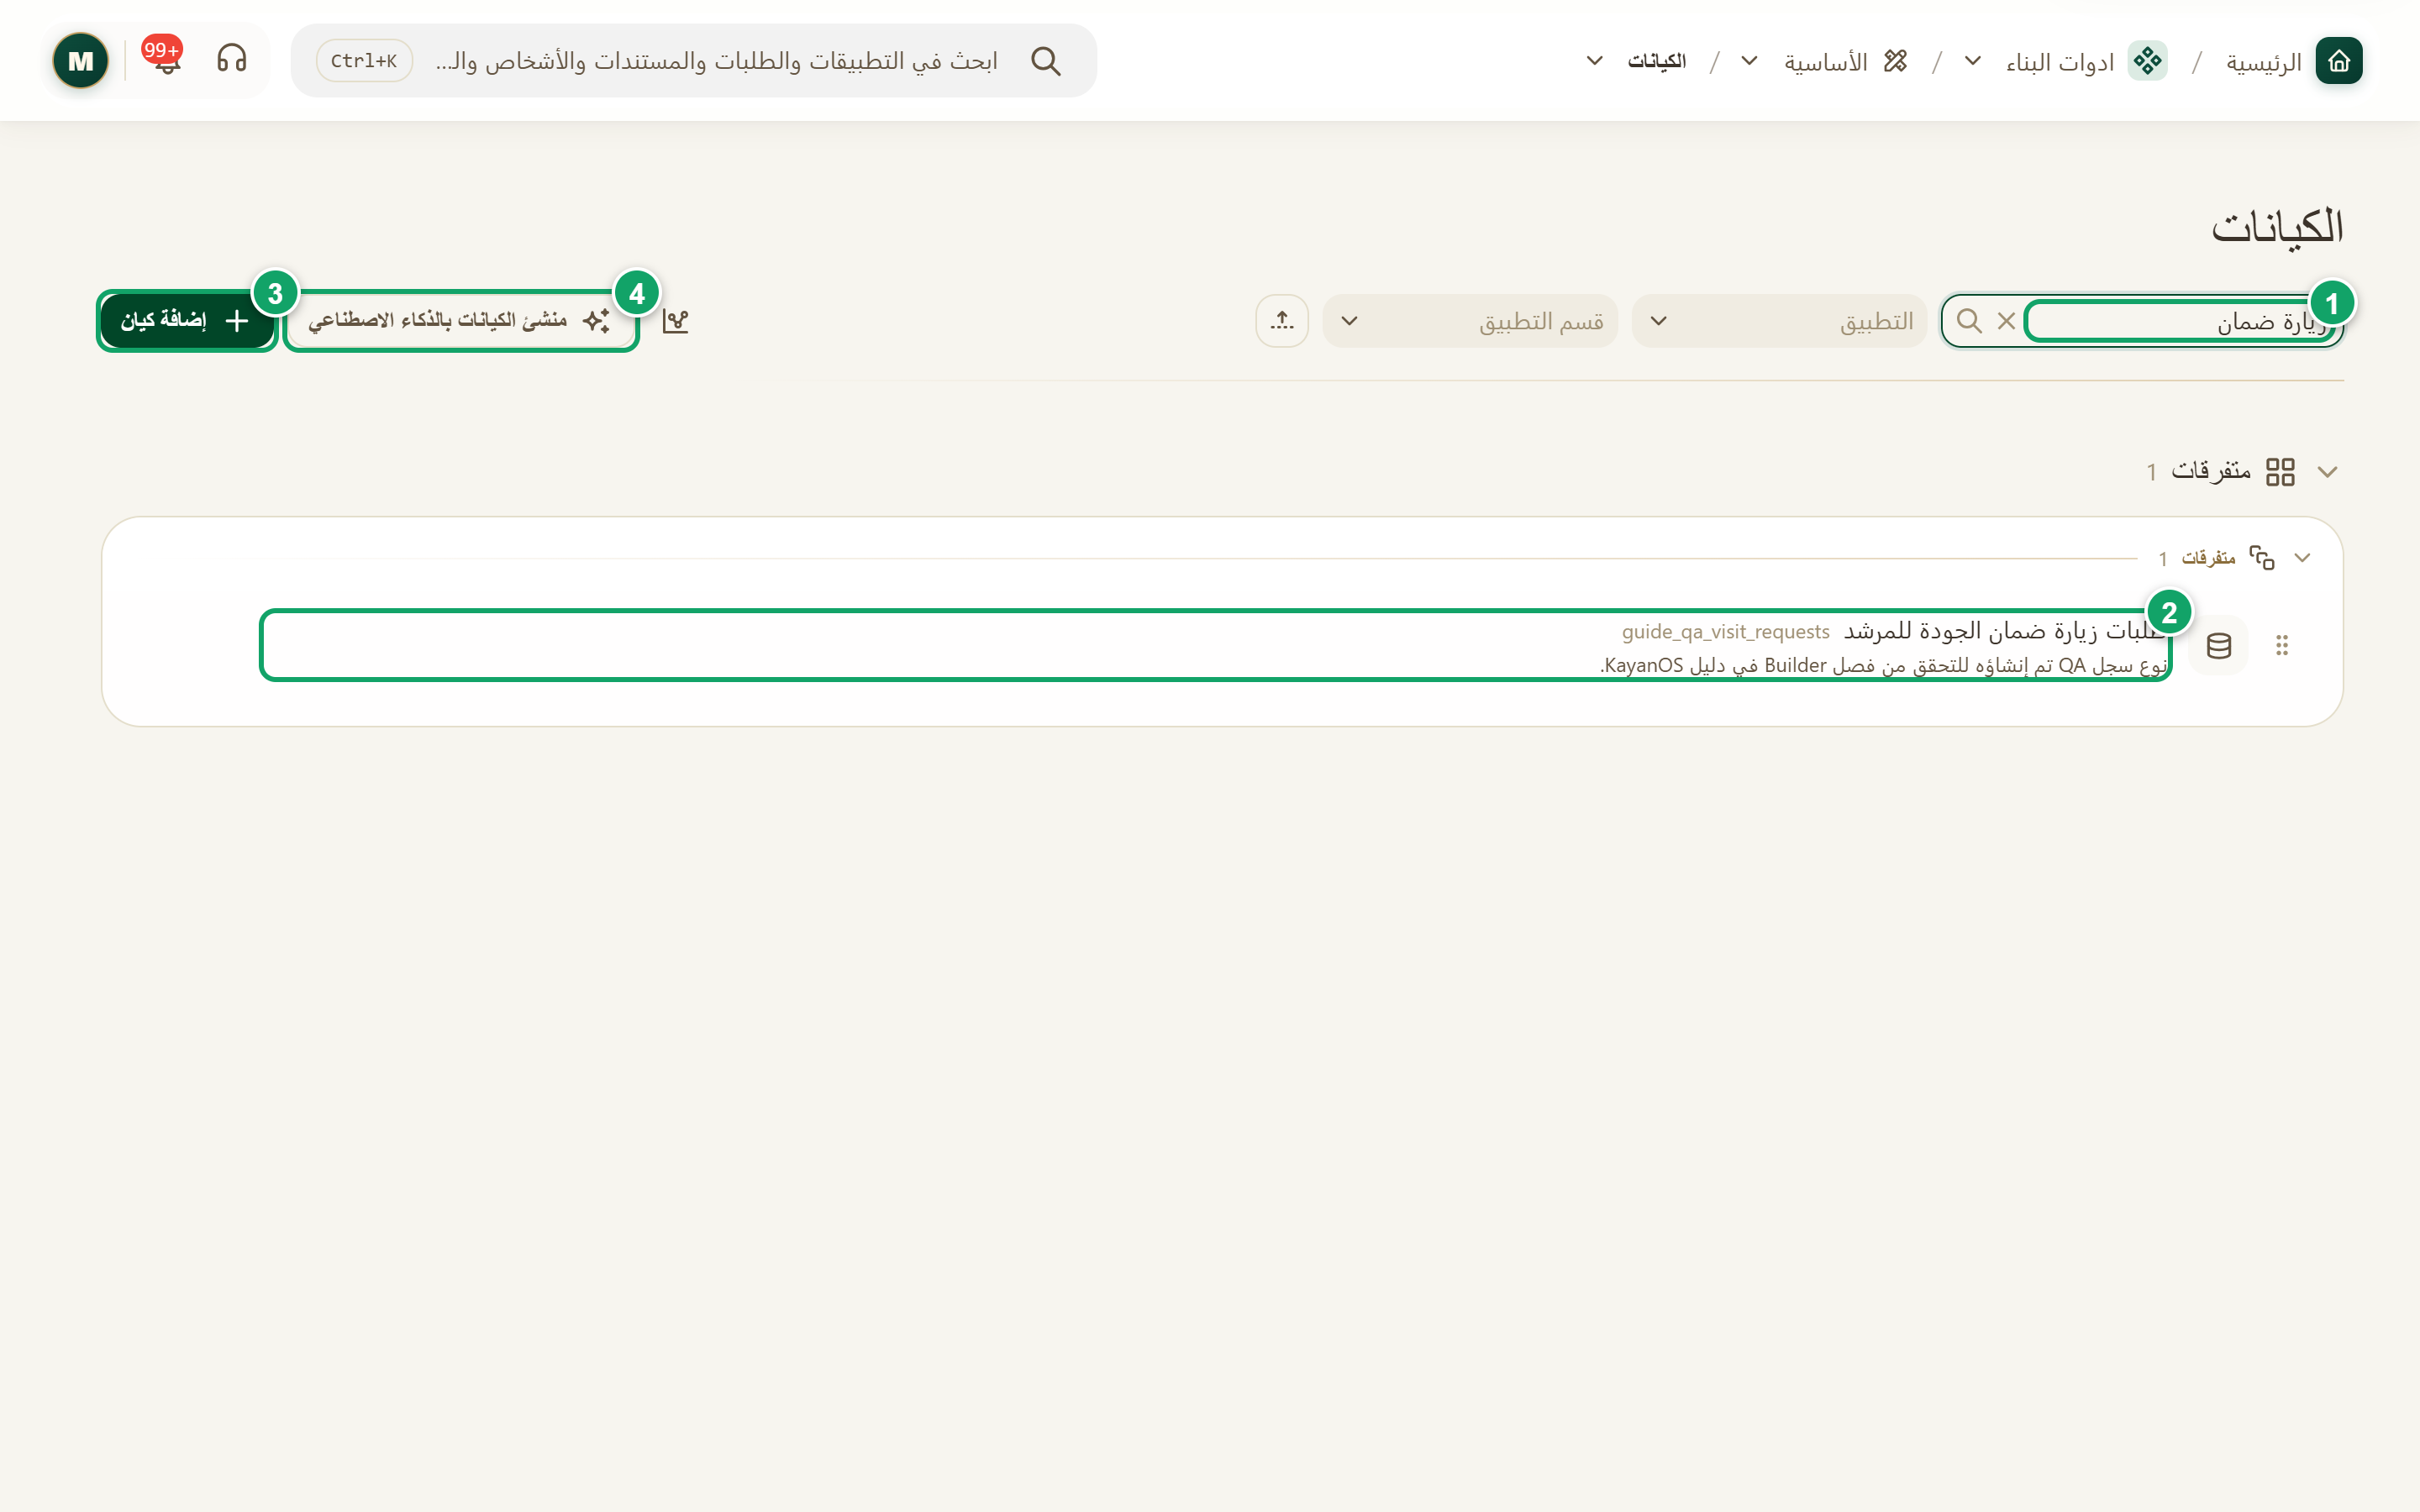
\includegraphics[width=0.95\linewidth,height=0.72\textheight,keepaspectratio]{figures/screens/ch06-entities-ar.png}
\caption{صفحة «الكيانات» بعد البحث عن نوع سجلات}
\label{fig:builder-entities-screen}
\shotnote{تعرض الصفحة أنواع السجلات مجمّعة حسب التطبيق، وهنا ضُيّقت القائمة بالبحث فظهر نوع سجلات اختباري واحد أُنشئ في test2 للتحقق من هذا الفصل. ① مربع البحث: اكتب جزءاً من اسم النوع قبل أن تنشئ نوعاً جديداً. ② النوع الذي وجدته: اضغطه لتفتحه في «المنشئ». ③ «إضافة كيان»: تنشئ نوعاً جديداً عندما لا تجد ما تحتاجه. ④ «منشئ الكيانات بالذكاء الاصطناعي»: يقترح الحقول من وصف تكتبه.}
\end{figure}


\begin{table}[H]
\centering
\caption{ما الذي تجده هنا؟}
\label{tab:builder-entities-data}
\begin{tabularx}{\linewidth}{R{3.6cm} Y}
\rcHeaderRow
\thh{القسم} & \thh{المحتوى والإجراء}\\
قائمة الأنواع & أنواع السجلات مجمّعة حسب التطبيق والقسم، ولكل نوع اسمه ومفتاحه ووصفه. تضيّق القائمة بالبحث أو بفلترَي «التطبيق» و«قسم التطبيق».\\
إضافة كيان & يفتح صفحة تكتب فيها عنوان النوع ووصفه وحقوله الأولى، ثم تضغط «انشاء كيان».\\
منشئ الكيانات بالذكاء الاصطناعي & تصف النوع الذي تريده بكلماتك، فيقترح النظام حقوله لتراجعها قبل الحفظ. يظهر الزر فقط إذا فعّلت المؤسسة الذكاء الاصطناعي في أدوات البناء.\\
عرض مخطط العلاقات & يرسم أنواع السجلات والعلاقات بينها، فتعرف ما يرتبط بالنوع قبل تعديله.\\
فتح نوع موجود & الضغط على النوع يفتحه في «المنشئ»، حيث تعدّل حقوله وصفحته وقوائمه وتنشر التغييرات.\\
\end{tabularx}
\end{table}

\begin{figure}[H]
\centering
\begin{tikzpicture}[node distance=0.5cm]
\node[stepBox] (a) {\RL{البحث عن نوع مشابه}};
\node[stepBox,below=of a] (b) {\RL{إضافة كيان وكتابة عنوانه}};
\node[stepBox,below=of b] (c) {\RL{انشاء كيان}};
\node[stepBox,below=of c] (d) {\RL{فتحه في المنشئ}};
\draw[flowsTo] (a) -- (b);
\draw[flowsTo] (b) -- (c);
\draw[flowsTo] (c) -- (d);
\end{tikzpicture}
\rclegend
\caption{خطوات إنشاء نوع سجلات}
\label{fig:builder-entities-flow}
\shotnote{يبدأ المخطط بالبحث لأن النوع الذي تحتاجه قد يكون موجوداً في تطبيق جاهز، وإنشاء نسخة ثانية منه يفرّق البيانات بين مكانين. وبعد «انشاء كيان» تعود إلى قائمة الكيانات، ثم تفتح النوع الجديد في «المنشئ» لتكمل بناءه، فالإنشاء لا يعني أن التطبيق صار جاهزاً للفريق.}
\end{figure}

\subsection{خطوات العمل والتحقق}
\begin{enumerate}
\item افتح «الكيانات» واكتب في البحث اسماً قريباً مما تحتاجه، ثم راجع النتائج قبل أن تنشئ نوعاً جديداً.
\item اضغط «إضافة كيان»، واكتب عنواناً بصيغة الجمع يصف السجلات، مثل «طلبات الصيانة»، ثم أضف وصفاً قصيراً.
\item سمِّ الحقل الأول المقترح أو غيّر نوعه، واضغط «اضافة حقل جديد» لكل معلومة أساسية أخرى.
\item اضغط زر الإعدادات بجانب «انشاء كيان» لتختار التطبيق والقسم اللذين يظهر فيهما النوع، ثم اضغط «انشاء كيان».
\end{enumerate}

\textbf{تحقق ومعالجة المشكلة:} يجب أن تظهر رسالة نجاح وأن يظهر النوع الجديد في قائمة «الكيانات» تحت التطبيق الذي اخترته. فإذا بقي زر «انشاء كيان» معطلاً، فاكتب عنوان النوع أولاً؛ وإذا لم تجد النوع في القائمة، فأزل فلترَي التطبيق والقسم وابحث باسمه.

\clearpage
\section{منشئ الكيانات بالذكاء الاصطناعي ومخطط العلاقات}
\label{sec:builder-feature-ai-builder}

بدلاً من إضافة الحقول واحداً بعد الآخر، يمكنك أن تصف نوع السجلات الذي تحتاجه بكلماتك، فيقترح «منشئ الكيانات بالذكاء الاصطناعي» حقوله وتبويباته وأقسامه، ثم تراجع الاقتراح وتعدّله قبل حفظه. وتفيدك هذه الطريقة عندما يكون النوع كبيراً أو عندما تريد نقطة بداية سريعة. أما «عرض مخطط العلاقات» فيرسم أنواع السجلات الموجودة والعلاقات بينها، فتعرف قبل أي تعديل ما الذي يرتبط بالنوع الذي ستغيّره.

\textbf{المسار ومن يستخدمه:} «الكيانات» ← «منشئ الكيانات بالذكاء الاصطناعي»، أو زر «عرض مخطط العلاقات» في رأس الصفحة نفسها. يظهر زر الذكاء الاصطناعي عندما يكون «الذكاء الاصطناعي في أدوات البناء» مفعّلاً في إعدادات المؤسسة، ويحتاج الحفظ إلى صلاحيات إنشاء الكيانات وتعديلها وإنشاء الحقول.

\begin{rcnote}[مثال: شركة الأفق]
يكتب مسؤول النظام في الأفق: «أنشئ نوع سجلات لطلبات زيارة الفروع، فيه الفرع وتاريخ الزيارة وغرضها ومقدّم الطلب». ثم يجيب عن سؤالين يطرحهما المساعد، ويراجع الحقول المقترحة، ويضغط «تحقق» قبل «حفظ الكيان».
\end{rcnote}

\begin{figure}[H]
\centering
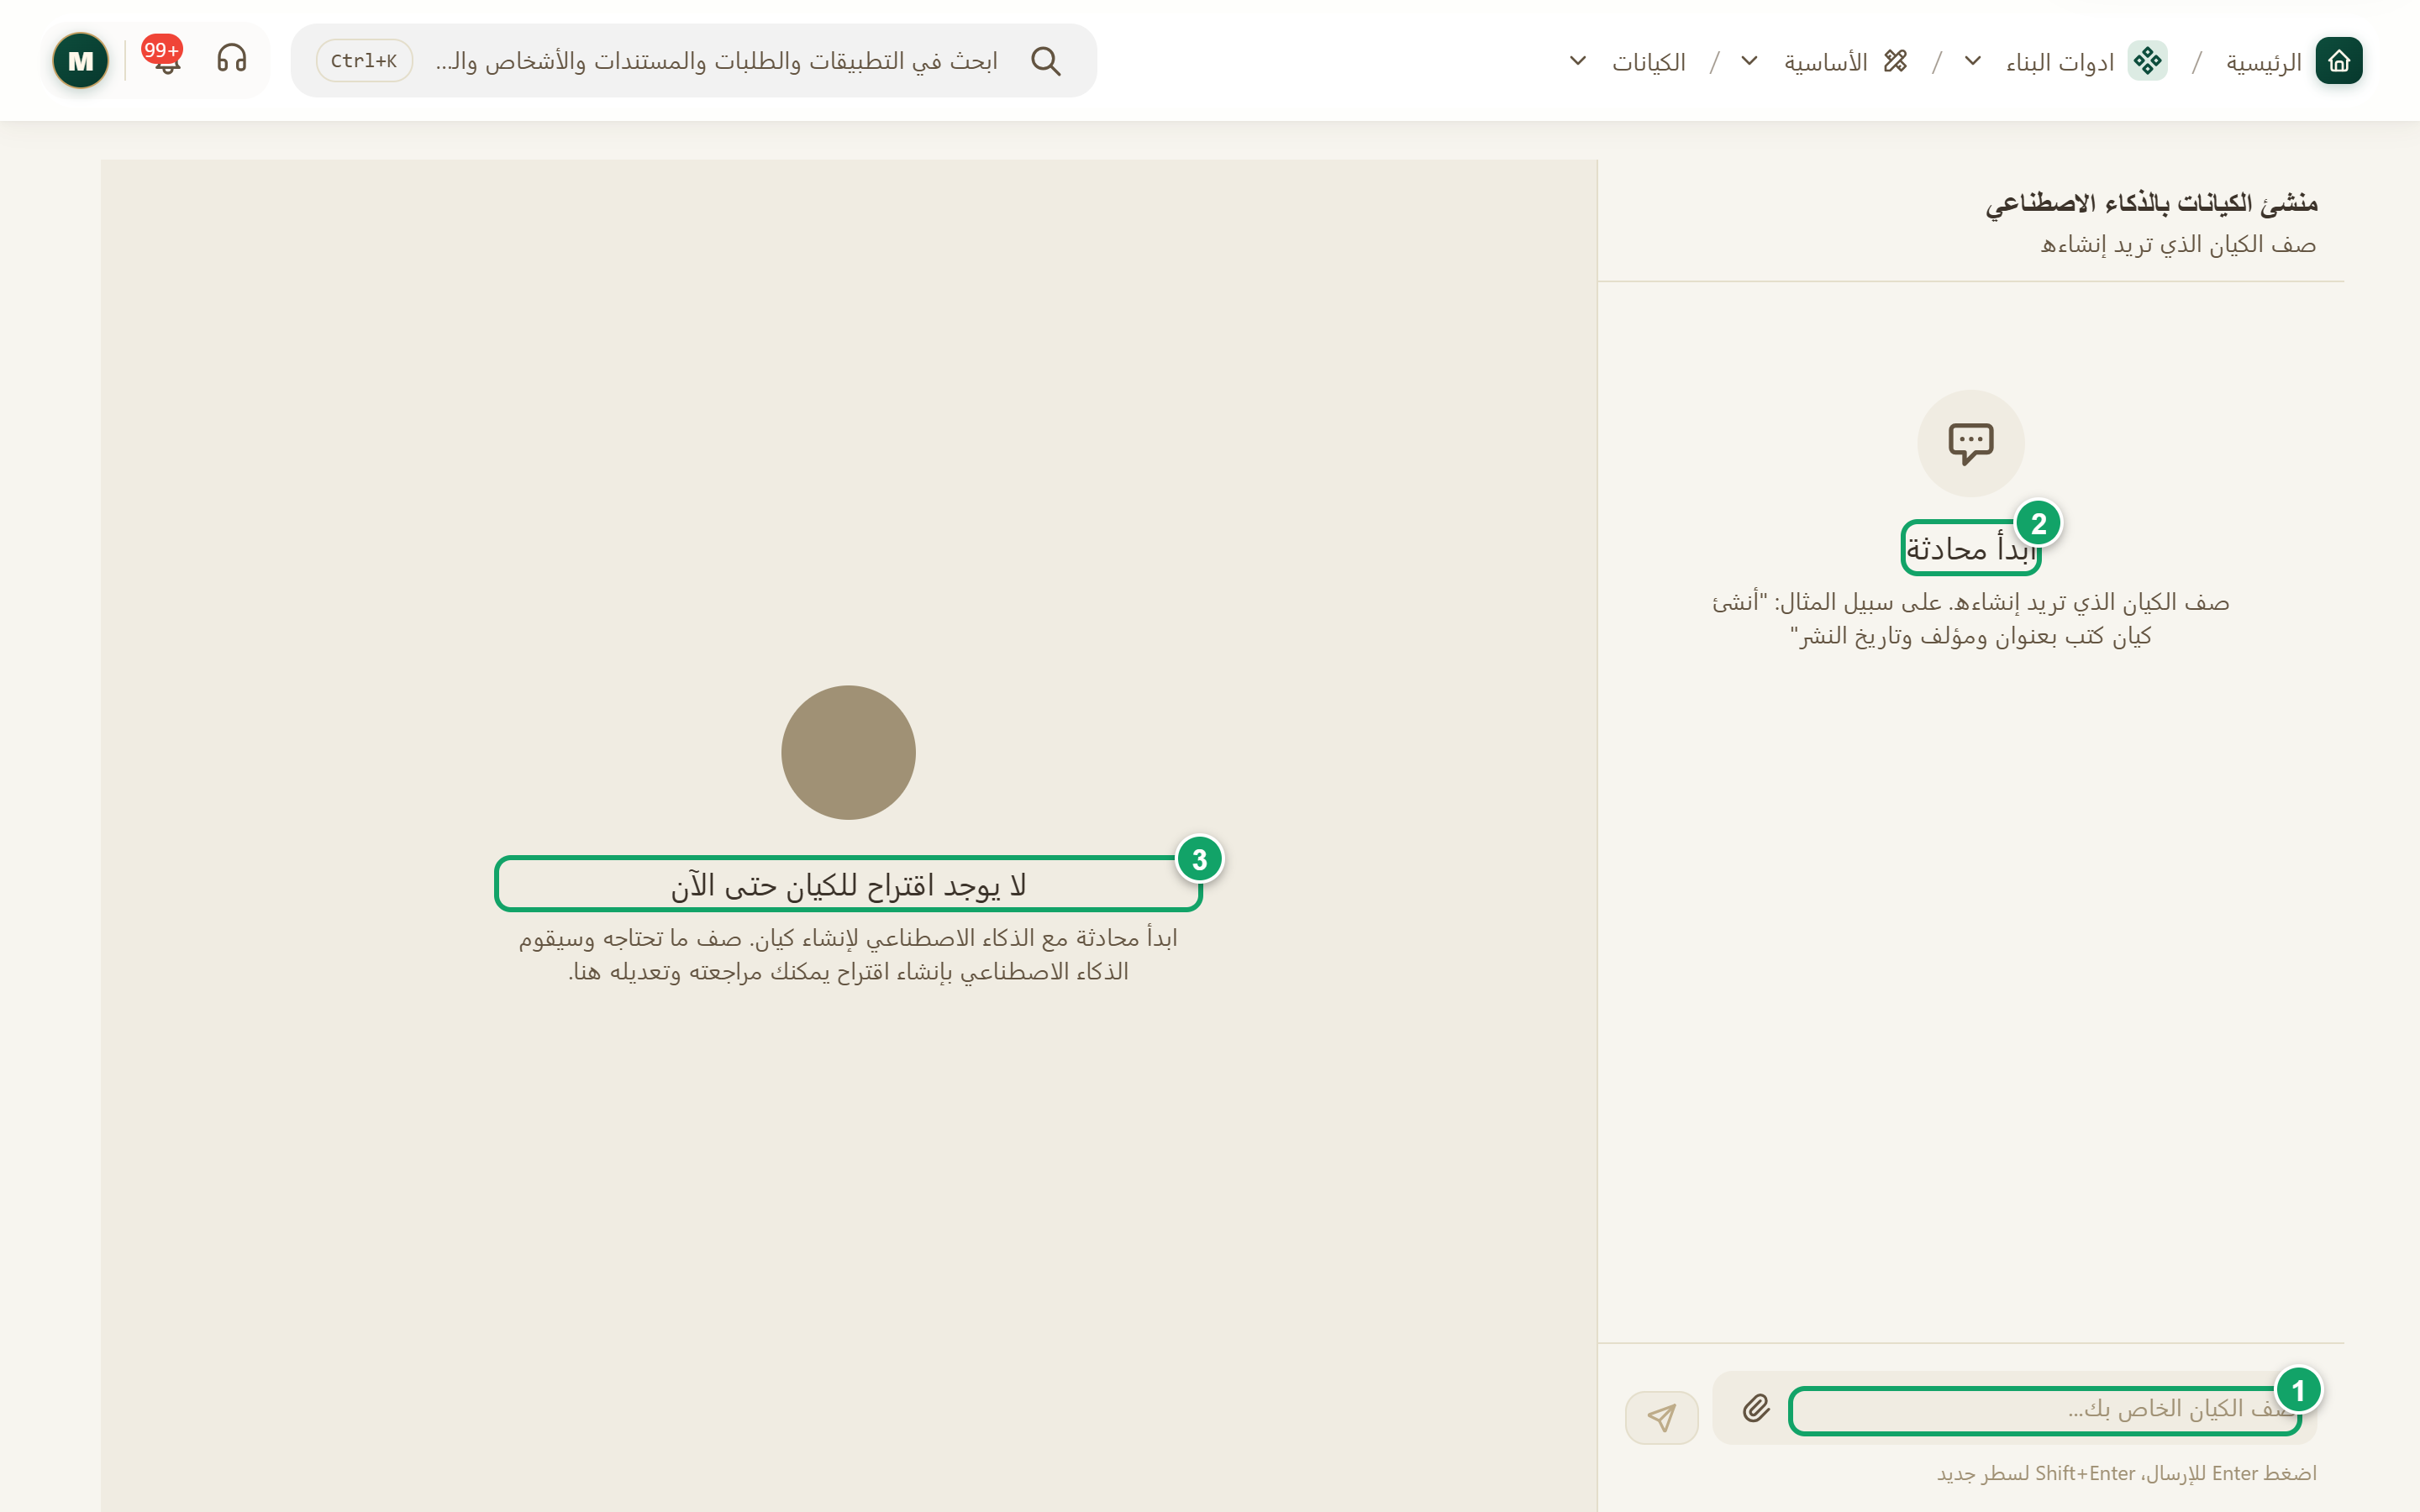
\includegraphics[width=0.95\linewidth,height=0.72\textheight,keepaspectratio]{figures/screens/ch06-ai-builder-ar.png}
\caption{منشئ الكيانات بالذكاء الاصطناعي قبل بدء المحادثة}
\label{fig:builder-ai-builder-screen}
\shotnote{تعرض الشاشة المساعد قبل أي محادثة: المحادثة في جهة، ومعاينة الاقتراح في الجهة الأخرى وهي فارغة حتى يقترح المساعد نوعاً. وتفيدك الصورة في معرفة مكان الكتابة ومكان مراجعة النتيجة قبل الحفظ. ① مربع «صف الكيان الخاص بك...»: تكتب فيه وصف النوع. ② «ابدأ محادثة»: مثال على وصف مناسب تسترشد به. ③ «لا يوجد اقتراح للكيان حتى الآن»: مكان «معاينة الكيان» الذي يمتلئ بعد أول اقتراح.}
\end{figure}

\begin{table}[H]
\centering
\caption{ما الذي تجده في المنشئ بالذكاء الاصطناعي؟}
\label{tab:builder-ai-builder-parts}
\begin{tabularx}{\linewidth}{R{3.6cm} Y}
\rcHeaderRow
\thh{الجزء} & \thh{ما يقدمه}\\
المحادثة & تصف النوع في مربع «صف الكيان الخاص بك...»، ويمكنك أن ترفق ملفاً يشرح عملك. وقد يطرح المساعد أسئلة توضيحية، فتجيب عنها ثم تضغط «إرسال الإجابات».\\
معاينة الكيان & تعرض الاقتراح كاملاً: المفتاح والعنوان والوصف، والتبويبات والأقسام، والإجراءات المخصصة، وجدول الحقول. ويمكنك أن تعدّل أي جزء منه قبل الحفظ.\\
تحقق & يفحص الاقتراح، ويعرض ما يجده في «مشاكل التحقق» مع اقتراح لإصلاح كل مشكلة. والأخطاء تمنع الحفظ، أما التحذيرات فلا تمنعه.\\
اطلب من الذكاء الاصطناعي الإصلاح & يرسل المشكلات إلى المحادثة، فيصحّح المساعد اقتراحه بدلاً من أن تعدّله يدوياً.\\
حفظ الكيان & ينشئ النوع وحقوله بعد «تأكيد الحفظ». ولا يعمل الزر إلا بعد تحقق ناجح دون أخطاء، وبعد آخر تعديل أجريته.\\
تحميل JSON & يحفظ الاقتراح ملفاً تحتفظ به أو تشاركه مع زميل للمراجعة.\\
مخطط العلاقات & يعرض كل نوع مع حقوله، ويرسم العلاقات أسهماً تحمل اسم الحقل الذي يربط بينها. والضغط على نوع يبرز علاقاته، و«تحميل البنية» يحفظ وصفاً نصياً لكل الأنواع وعلاقاتها.\\
\end{tabularx}
\end{table}

\begin{rcwarn}[الحفظ هنا لا يمر بمسودة]
على خلاف «المنشئ»، يُنشأ النوع وحقوله مباشرة بعد «تأكيد الحفظ»، ثم تعود إلى قائمة «الكيانات». لذلك راجع الاقتراح جيداً قبل الحفظ، ثم افتح النوع في «المنشئ» لتكمل صفحته وقواعده وصلاحياته. وإذا كان الاقتراح يعدّل نوعاً موجوداً، فالحفظ يضيف الحقول الجديدة فقط ولا يغيّر الحقول القائمة.
\end{rcwarn}

\begin{figure}[H]
\centering
\begin{tikzpicture}[node distance=0.5cm]
\node[stepBox] (a) {\RL{وصف النوع في المحادثة}};
\node[stepBox,below=of a] (b) {\RL{الإجابة عن الأسئلة}};
\node[stepBox,below=of b] (c) {\RL{مراجعة معاينة الكيان}};
\node[stepBox,below=of c] (d) {\RL{تحقق}};
\node[stepBox,below=of d] (e) {\RL{حفظ الكيان}};
\node[stepBox,below=of e] (f) {\RL{إكماله في المنشئ}};
\draw[flowsTo] (a) -- (b);
\draw[flowsTo] (b) -- (c);
\draw[flowsTo] (c) -- (d);
\draw[flowsTo] (d) -- (e);
\draw[flowsTo] (e) -- (f);
\end{tikzpicture}
\rclegend
\caption{إنشاء نوع سجلات بمساعدة الذكاء الاصطناعي}
\label{fig:builder-ai-builder-flow}
\shotnote{يضع المخطط «تحقق» قبل الحفظ لأن الزر لا يعمل دونه، ولأن كل تعديل في المعاينة يتطلب تحققاً جديداً. أما الخطوة الأخيرة فتذكّرك بأن المساعد يقترح الحقول والتبويبات فقط، وأن صفحة السجل وقواعده وصلاحياته تُضبط بعد ذلك في «المنشئ».}
\end{figure}

\subsection{خطوات العمل والتحقق}
\begin{enumerate}
\item افتح «الكيانات» واضغط «عرض مخطط العلاقات»، وابحث عن نوع قريب مما تحتاجه حتى لا تكرر نوعاً موجوداً.
\item اضغط «منشئ الكيانات بالذكاء الاصطناعي»، واكتب وصفاً يذكر ما يمثله السجل والمعلومات التي يحفظها، ثم اضغط \en{Enter}.
\item أجب عن الأسئلة التوضيحية إن ظهرت، واضغط «إرسال الإجابات».
\item راجع «معاينة الكيان»: اسم النوع ومفتاحه، وأنواع الحقول، والتبويبات. وعدّل ما يلزم مباشرة أو اطلب التعديل في المحادثة.
\item اضغط «تحقق»، وأصلح الأخطاء بنفسك أو بزر «اطلب من الذكاء الاصطناعي الإصلاح»، ثم اضغط «حفظ الكيان» و«تأكيد الحفظ».
\end{enumerate}

\textbf{تحقق ومعالجة المشكلة:} يجب أن تظهر رسالة «تم حفظ الكيان بنجاح» وأن يظهر النوع في قائمة «الكيانات». فإذا بقي «حفظ الكيان» معطلاً، فاضغط «تحقق» مرة أخرى بعد آخر تعديل، أو مرّر المؤشر فوقه لترى الصلاحيات الناقصة. وإذا لم يظهر زر الذكاء الاصطناعي أصلاً، فاطلب من مسؤول المؤسسة تفعيل «الذكاء الاصطناعي في أدوات البناء».

\clearpage
\section{المنشئ والنظرة العامة}
\label{sec:builder-feature-workspace}

«المنشئ» هو مساحة العمل التي تعدّل فيها نوع السجلات بعد إنشائه، وتفتحه بالضغط على النوع في صفحة «الكيانات». وتظهر أقسامه في قائمة جانبية بالترتيب: «نظرة عامة»، و«الحقول»، و«صفحة السجل»، و«القوائم وطرق العرض»، و«القواعد»، و«الصلاحيات»، و«الحركة»، و«الإثبات»، و«الإجراءات والأتمتة»، و«الاستيراد»، و«إعدادات متقدمة». ويلخّص قسم «نظرة عامة» حالة النوع كلها في مكان واحد، وينبّهك إلى ما يجب إصلاحه قبل النشر.

\textbf{المسار ومن يستخدمه:} «الكيانات» ← اضغط نوع السجلات ← «نظرة عامة». يستخدمه من يبني النوع في كل مرة يعود إليه، ليعرف ما تغيّر وما بقي ناقصاً.

\begin{rcnote}[مثال: شركة الأفق]
يفتح المسؤول «طلبات الزيارة» فيرى في «نظرة عامة» أن ثلاثة حقول لم توضع بعد في أي صفحة، وأن قائمة «قبل النشر» تعرض تحذيراً لتسمية بلا نص إنجليزي. فيضع الحقول في الصفحة ويترجم التسمية، ثم يضغط «المراجعة والنشر».
\end{rcnote}

\begin{figure}[H]
\centering
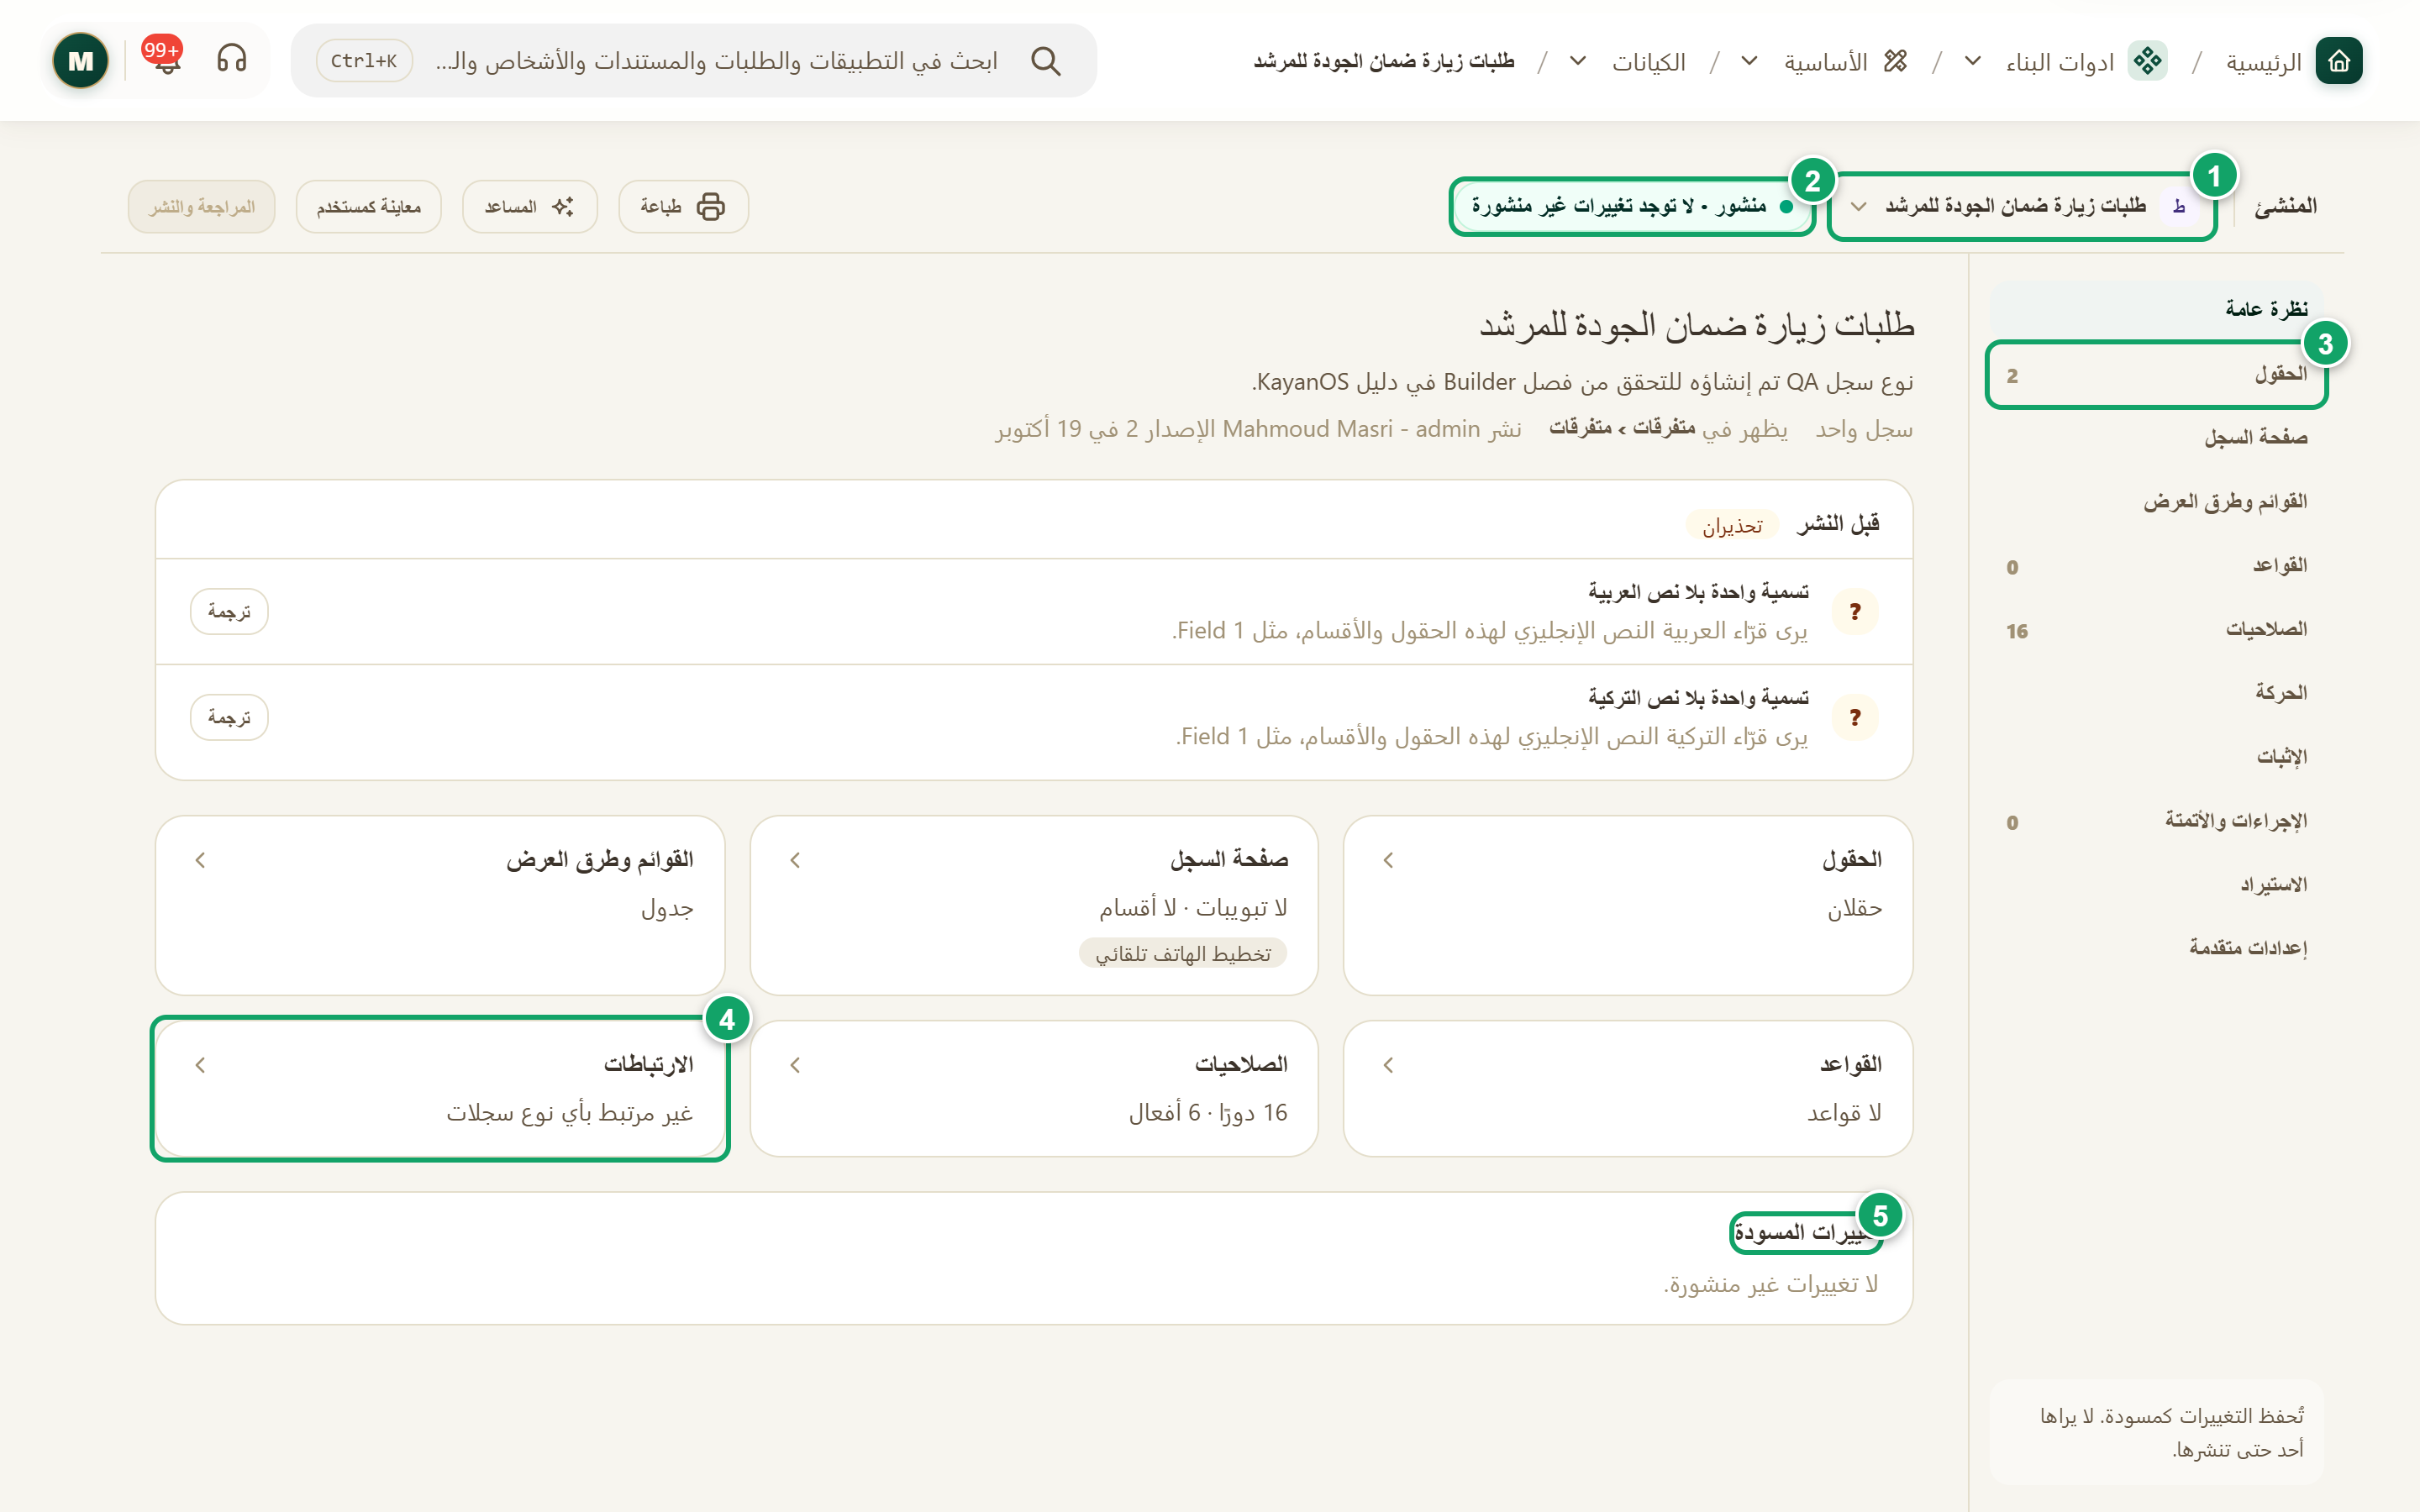
\includegraphics[width=0.95\linewidth,height=0.72\textheight,keepaspectratio]{figures/screens/ch06-ws-header-ar.png}
\caption{رأس المنشئ وقسم «نظرة عامة» لنوع سجلات اختباري}
\label{fig:builder-workspace-screen}
\shotnote{تعرض الصورة نوع السجلات الاختباري الذي أُنشئ في test2 للتحقق من هذا الدليل، مفتوحاً في «المنشئ» على «نظرة عامة». ويجمع الرأس والقائمة الجانبية والبطاقات كل ما تحتاج إلى معرفته قبل أي تعديل. ① تبديل نوع السجلات. ② شارة الحالة: تقول إن النوع منشور ولا تغييرات معلّقة. ③ «الحقول» في القائمة الجانبية: الرقم بجانبها عدد الحقول. ④ بطاقة «الارتباطات». ⑤ «تغييرات المسودة»: ما لم يُنشر بعد.}
\end{figure}

\begin{table}[H]
\centering
\caption{رأس المنشئ}
\label{tab:builder-workspace-header}
\begin{tabularx}{\linewidth}{R{3.6cm} Y}
\rcHeaderRow
\thh{العنصر} & \thh{ما يقدمه}\\
تبديل نوع السجلات & ينقلك إلى نوع آخر دون العودة إلى القائمة، وفيه بحث «ابحث عن نوع سجلات».\\
شارة الحالة & تقول «منشور · لا توجد تغييرات غير منشورة» عندما يطابق النوع ما يراه الفريق، أو «مسودة» مع عدد التغييرات غير المنشورة ووقت آخر حفظ.\\
طباعة & يفتح قوالب الطباعة الخاصة بنوع السجلات، ويظهر عددها بجانب الزر عند وجودها.\\
المساعد & يفتح «مساعد البناء»، فتطلب منه حقلاً أو قاعدة أو معادلة، فيقترح تغييرات على المسودة وتطبّق منها ما تريد. ولا يُنشر شيء حتى تراجع وتنشر.\\
معاينة كمستخدم & تعرض صفحة السجل كما يراها دور أو شخص بعينه، دون أن يُحفظ شيء.\\
المراجعة والنشر · N & يفتح نافذة المراجعة، والرقم عدد التغييرات في المسودة. ولا يعمل الزر إذا لم تكن هناك تغييرات.\\
\end{tabularx}
\end{table}

\begin{table}[H]
\centering
\caption{أجزاء «نظرة عامة»}
\label{tab:builder-workspace-cards}
\begin{tabularx}{\linewidth}{R{3.6cm} Y}
\rcHeaderRow
\thh{الجزء} & \thh{ما يخبرك به}\\
رأس الصفحة & اسم النوع ووصفه، وعدد السجلات، والتطبيق والقسم في «يظهر في»، والإصدار المنشور ومن نشره. ومنه تفتح قائمة السجلات بزر «فتح القائمة».\\
الحقول & عدد الحقول، والمحسوبة والمجمّعة منها، والحقول التي لم توضع في أي صفحة.\\
صفحة السجل & عدد التبويبات والأقسام، وهل كتل النظرة العامة مفعّلة.\\
القوائم وطرق العرض & طرق العرض المتاحة والافتراضية منها، وعدد المؤشرات والعروض المحفوظة.\\
القواعد & عدد القواعد موزعاً حسب نوعها، مثل الإظهار والإخفاء والتعديل والإلزام.\\
الصلاحيات & عدد الأدوار والأفعال والأفعال المخصصة، والحقول التي لها صلاحيات خاصة.\\
الارتباطات & عدد أنواع السجلات المرتبطة بهذا النوع، فتعرف ما قد يتأثر بتعديله.\\
تغييرات المسودة & التغييرات غير المنشورة منذ بدء المسودة، ومنها تفتح المراجعة بزر «مراجعة الكل».\\
قبل النشر & المشكلات التي تمنع النشر والتحذيرات، ولكل مشكلة زر يفتح مكان إصلاحها.\\
\end{tabularx}
\end{table}

\subsection{قائمة «قبل النشر»}

تفحص هذه القائمة المسودة كلما عدّلتها. فبعض المشكلات يمنع النشر لأن السجلات لن تعمل معها، مثل قاعدة أو صيغة تشير إلى حقل محذوف، أو تعبير فيه خطأ، أو خيارات قائمة فارغة أو مكررة، أو حذف الحقل الذي يحمل اسم السجل. أما التحذيرات فلا تمنع النشر لكنها تستحق المراجعة، مثل تبويب يبقى فارغاً دائماً، أو حقل وُضع في تبويب غير موجود، أو تسميات بلا ترجمة. وعندما تخلو القائمة يظهر «لا شيء يحتاج إلى إصلاح. يمكن نشر المسودة.».

\begin{rcwarn}[عندما يعدّل شخصان المسودة نفسها]
إذا حفظ شخص آخر المسودة بعد أن فتحتها، تظهر رسالة «غيّر شخص آخر هذه المسودة»، ولا تُحفظ تعديلاتك حتى تختار. اضغط «تحميل مسودته» لترى نسخته وتفقد تعديلاتك غير المحفوظة، أو «استبدالها بنسختي» لتحفظ نسختك فوقها. وقد ظهرت هذه الرسالة أثناء اختبار هذا الدليل لنسخة قديمة من الجلسة نفسها، فإن كنت متأكداً أن أحداً لا يعدّل النوع معك فاختر «استبدالها بنسختي».
\end{rcwarn}

\begin{figure}[H]
\centering
\begin{tikzpicture}[node distance=0.5cm]
\node[stepBox] (a) {\RL{فتح النوع من الكيانات}};
\node[stepBox,below=of a] (b) {\RL{قراءة نظرة عامة}};
\node[stepBox,below=of b] (c) {\RL{التعديل في الأقسام}};
\node[stepBox,below=of c] (d) {\RL{إصلاح ما في قبل النشر}};
\node[stepBox,below=of d] (e) {\RL{المراجعة والنشر}};
\draw[flowsTo] (a) -- (b);
\draw[flowsTo] (b) -- (c);
\draw[flowsTo] (c) -- (d);
\draw[flowsTo] (d) -- (e);
\end{tikzpicture}
\rclegend
\caption{جلسة عمل في المنشئ}
\label{fig:builder-workspace-flow}
\shotnote{يبدأ المخطط بقراءة «نظرة عامة» لأنها تبيّن لك حالة النوع قبل أن تغيّر شيئاً، وينتهي بالنشر لأن التعديلات تبقى في المسودة حتى ذلك الحين. وتقع خطوة «قبل النشر» قبل المراجعة مباشرة، لأن مشكلة واحدة تمنع النشر كله حتى تُصلحها.}
\end{figure}

\subsection{خطوات العمل والتحقق}
\begin{enumerate}
\item افتح «الكيانات» واضغط نوع السجلات، فيفتح «المنشئ» على «نظرة عامة».
\item اقرأ شارة الحالة: إذا كانت «مسودة» فهناك تغييرات سابقة لم تُنشر، فراجعها من «تغييرات المسودة» قبل أن تضيف غيرها.
\item انتقل إلى القسم الذي تريد تعديله من القائمة الجانبية، وعدّل ما تحتاج إليه؛ فكل تعديل يُحفظ في المسودة تلقائياً.
\item عُد إلى «نظرة عامة»، واضغط زر الإصلاح بجانب كل مشكلة في «قبل النشر» حتى تخلو القائمة من الأخطاء.
\end{enumerate}

\textbf{تحقق ومعالجة المشكلة:} يجب أن تتغير شارة الحالة إلى «مسودة» مع عدد التغييرات بعد كل تعديل، وأن يصبح زر «المراجعة والنشر» متاحاً. فإذا ظهر «تعذّر الحفظ، سنعيد المحاولة عند التغيير التالي»، فتحقق من اتصالك ثم عدّل أي قيمة ليُعاد الحفظ.

\clearpage
\section{الحقول}
\label{sec:builder-feature-fields}

يحدد الحقل معلومة واحدة يحفظها كل سجل، مثل التاريخ أو المبلغ أو الشخص المسؤول. واختيار نوع الحقل المناسب مهم، لأنه يحدد طريقة الإدخال والتحقق من القيمة، ويسمح بالترتيب والتصفية والحساب لاحقاً. وتضيف الحقول من قسم «الحقول» في «المنشئ».

\textbf{المسار ومن يستخدمه:} «الكيانات» ← افتح نوع السجلات ← «الحقول». يستخدمه من يبني نوع السجلات، قبل ترتيب الصفحة والقوائم.

\begin{rcnote}[مثال: شركة الأفق]
يضيف مسؤول النظام إلى «طلبات الزيارة» حقل «معرف تسلسلي» يعطي كل طلب رقماً مثل \en{HZN-VR-0001}، ثم حقل «علاقة» يربط الطلب بالفرع، وحقل «تاريخ» لموعد الزيارة، وحقل «نص طويل» لغرضها. وتطابق خطواته في الصورة الرقمين ① و③.
\end{rcnote}

\begin{figure}[H]
\centering
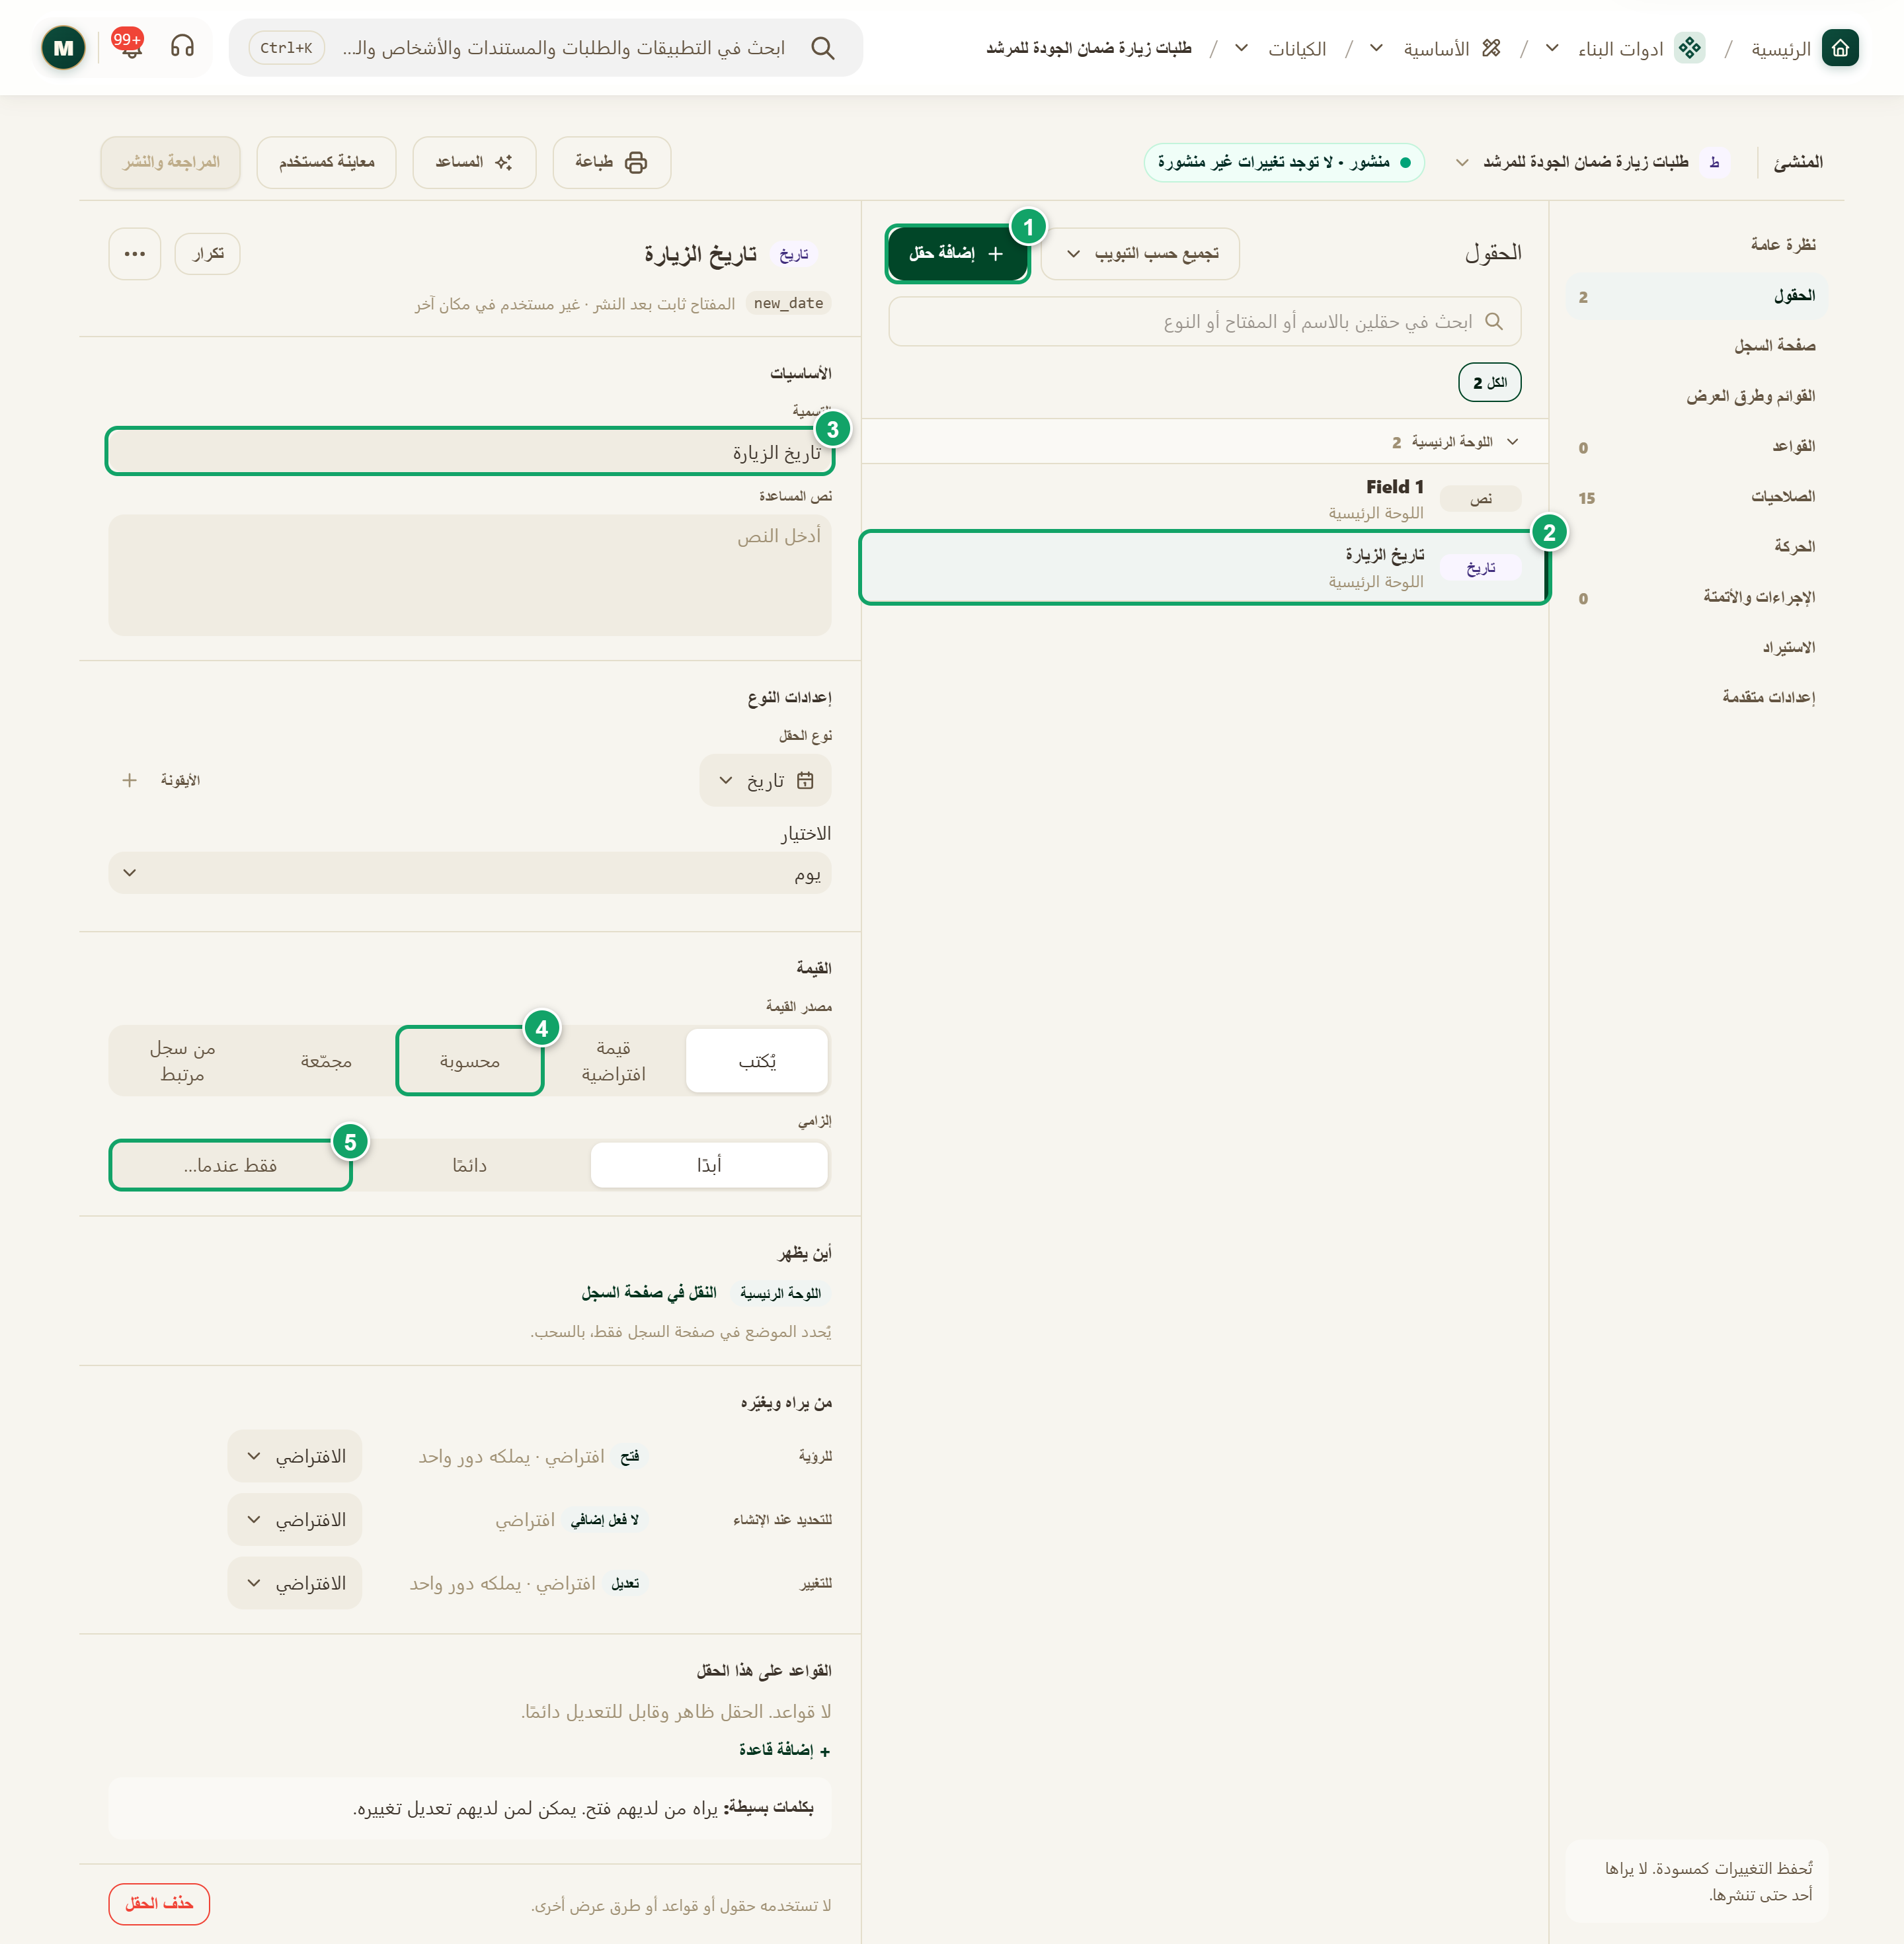
\includegraphics[width=0.95\linewidth,height=0.72\textheight,keepaspectratio]{figures/screens/ch06-ws-fields-ar.png}
\caption{قسم «الحقول» وإعدادات حقل تاريخ}
\label{fig:builder-fields-screen}
\shotnote{يعرض القسم قائمة حقول نوع السجلات، وعند اختيار حقل تظهر إعداداته بجانبه. والحقل المختار هنا حقل «تاريخ» أُضيف ونُشر أثناء اختبار هذا الفصل على test2. ① «إضافة حقل». ② الحقل المختار في القائمة. ③ «التسمية». ④ «محسوبة»: تجعل القيمة ناتج صيغة بدلاً من أن يكتبها المستخدم. ⑤ «فقط عندما…»: تجعل الحقل إلزامياً في حالة معينة.}
\end{figure}


\begin{table}[H]
\centering
\caption{أنواع الحقول}
\label{tab:builder-fields-types}
\begin{tabularx}{\linewidth}{R{3.6cm} Y}
\rcHeaderRow
\thh{المجموعة} & \thh{الأنواع ومتى تستخدمها}\\
النصوص & «نص» لقيمة قصيرة، و«نص طويل» للوصف، و«نص منسّق» لنص بتنسيق، و«هاتف» لرقم الهاتف.\\
الأرقام والمعرّفات & «رقم» للكميات والمبالغ، و«المدة» للزمن المستغرق، و«معرف تسلسلي» لرقم مرجعي يولّده النظام لكل سجل.\\
التواريخ والأوقات & «تاريخ» و«تاريخ ووقت» و«وقت»، والنطاقات منها مثل «نطاق التاريخ» عندما يكون للمعلومة بداية ونهاية.\\
الاختيار والحالة & «اختيار» لقائمة قيم محددة، و«قيمة منطقية» لإجابة نعم أو لا، و«الحالة» لمراحل العمل وفق قالب حالات.\\
الملفات والصور & «ملف» للمرفقات، و«صورة رمزية» لصورة تمثّل السجل.\\
الروابط والأشخاص & «علاقة» لربط السجل بسجل من نوع آخر، و«اختيار عضو» لتحديد عضو من المؤسسة.\\
الخرائط & «موقع» لنقطة على الخريطة، و«حدود» لمساحة مرسومة مثل حدود عقار أو منشأة.\\
إجراء & حقل متقدم يعمل مع قسم «الإجراءات والأتمتة».\\
محسوبة ومرتبطة ومجمّعة & قيم لا يكتبها المستخدم: «محسوبة» بصيغة من حقول السجل، و«مرتبطة» تعرض قيمة من سجل مرتبط، و«مجمّعة» تجمع قيم السجلات المرتبطة أو تعدّها.\\
\end{tabularx}
\end{table}

\begin{table}[H]
\centering
\caption{ما الذي تضبطه في كل حقل؟}
\label{tab:builder-fields-settings}
\begin{tabularx}{\linewidth}{R{3.6cm} Y}
\rcHeaderRow
\thh{الإعداد} & \thh{المعنى}\\
التسمية & الاسم الذي يراه المستخدم، ويمكن كتابته بأكثر من لغة.\\
المفتاح & اسم ثابت يستخدمه النظام في الصيغ والقوالب. اختره واضحاً من البداية، لأن الإشارات إليه تعتمد عليه.\\
نص المساعدة & جملة قصيرة تشرح للمستخدم ما يكتبه في الحقل.\\
إلزامي & يمنع حفظ السجل إذا بقي الحقل فارغاً. استخدمه للمعلومات التي لا يكتمل العمل دونها فقط.\\
\end{tabularx}
\end{table}

\begin{figure}[H]
\centering
\begin{tikzpicture}[node distance=0.5cm]
\node[stepBox] (a) {\RL{إضافة حقل}};
\node[stepBox,below=of a] (b) {\RL{اختيار نوع الحقل}};
\node[stepBox,below=of b] (c) {\RL{التسمية والمفتاح}};
\node[stepBox,below=of c] (d) {\RL{الإلزام ونص المساعدة}};
\draw[flowsTo] (a) -- (b);
\draw[flowsTo] (b) -- (c);
\draw[flowsTo] (c) -- (d);
\end{tikzpicture}
\rclegend
\caption{خطوات إضافة حقل}
\label{fig:builder-fields-flow}
\shotnote{يضع المخطط اختيار النوع قبل التسمية، لأن النوع يحدد الإعدادات التي تظهر بعده، مثل خيارات القائمة في «اختيار» أو النوع المرتبط في «علاقة». وتُحفظ كل إضافة في المسودة فوراً، لكن المستخدمين لا يرون الحقل الجديد حتى تنشر التغييرات.}
\end{figure}

\subsection{خطوات العمل والتحقق}
\begin{enumerate}
\item افتح نوع السجلات من «الكيانات»، ثم اختر قسم «الحقول».
\item اضغط «إضافة حقل»، واختر النوع الذي يطابق المعلومة؛ فالتاريخ مثلاً يُحفظ في حقل «تاريخ» لا في «نص».
\item اكتب التسمية وراجع المفتاح، وأضف نص مساعدة عند الحاجة، ثم حدد إن كان الحقل إلزامياً.
\item لحقل يُحسب من غيره، اختر «محسوبة» واكتب الصيغة؛ ولقيمة من سجل مرتبط، اختر «حقل مرتبط» بعد إضافة حقل «علاقة».
\end{enumerate}

\textbf{تحقق ومعالجة المشكلة:} يجب أن يظهر الحقل في قائمة الحقول، وأن تعرض «نظرة عامة» عدده مع الحقول التي لم توضع بعد في أي صفحة. فإذا اخترت نوعاً خاطئاً، فصحّحه قبل النشر وقبل إدخال سجلات حقيقية، لأن تغيير النوع بعد تراكم البيانات أصعب.

\clearpage
\section{أنواع الحقول وإعداداتها}
\label{sec:builder-feature-field-types}

يحدد نوع الحقل شكل الإدخال، والتحقق من القيمة، وما يمكن فعله بها لاحقاً من ترتيب وتصفية وحساب. ولذلك تشرح هذه الصفحة كل الأنواع المتاحة في «إضافة حقل»، ثم الإعدادات الإضافية التي تظهر في «إعدادات النوع» لبعضها. واختر النوع قبل إدخال بيانات حقيقية، لأن تغييره بعد تراكم السجلات أصعب.

\textbf{المسار ومن يستخدمه:} «المنشئ» ← «الحقول» ← «إضافة حقل»، ثم «إعدادات النوع» في لوحة إعدادات الحقل. يستخدمه من يبني نوع السجلات.

\begin{rcnote}[مثال: شركة الأفق]
يختار مسؤول النظام لحقل رقم الطلب نوع «معرف تسلسلي» بوضع «تلقائي»، ويكتب له تنسيقاً يبدأ بـ \en{HZN-VR-} فيحمل أول طلب الرقم \en{HZN-VR-0001}. ويختار لحقل الفرع نوع «علاقة» يرتبط بنوع سجلات الفروع.
\end{rcnote}

\begin{figure}[H]
\centering
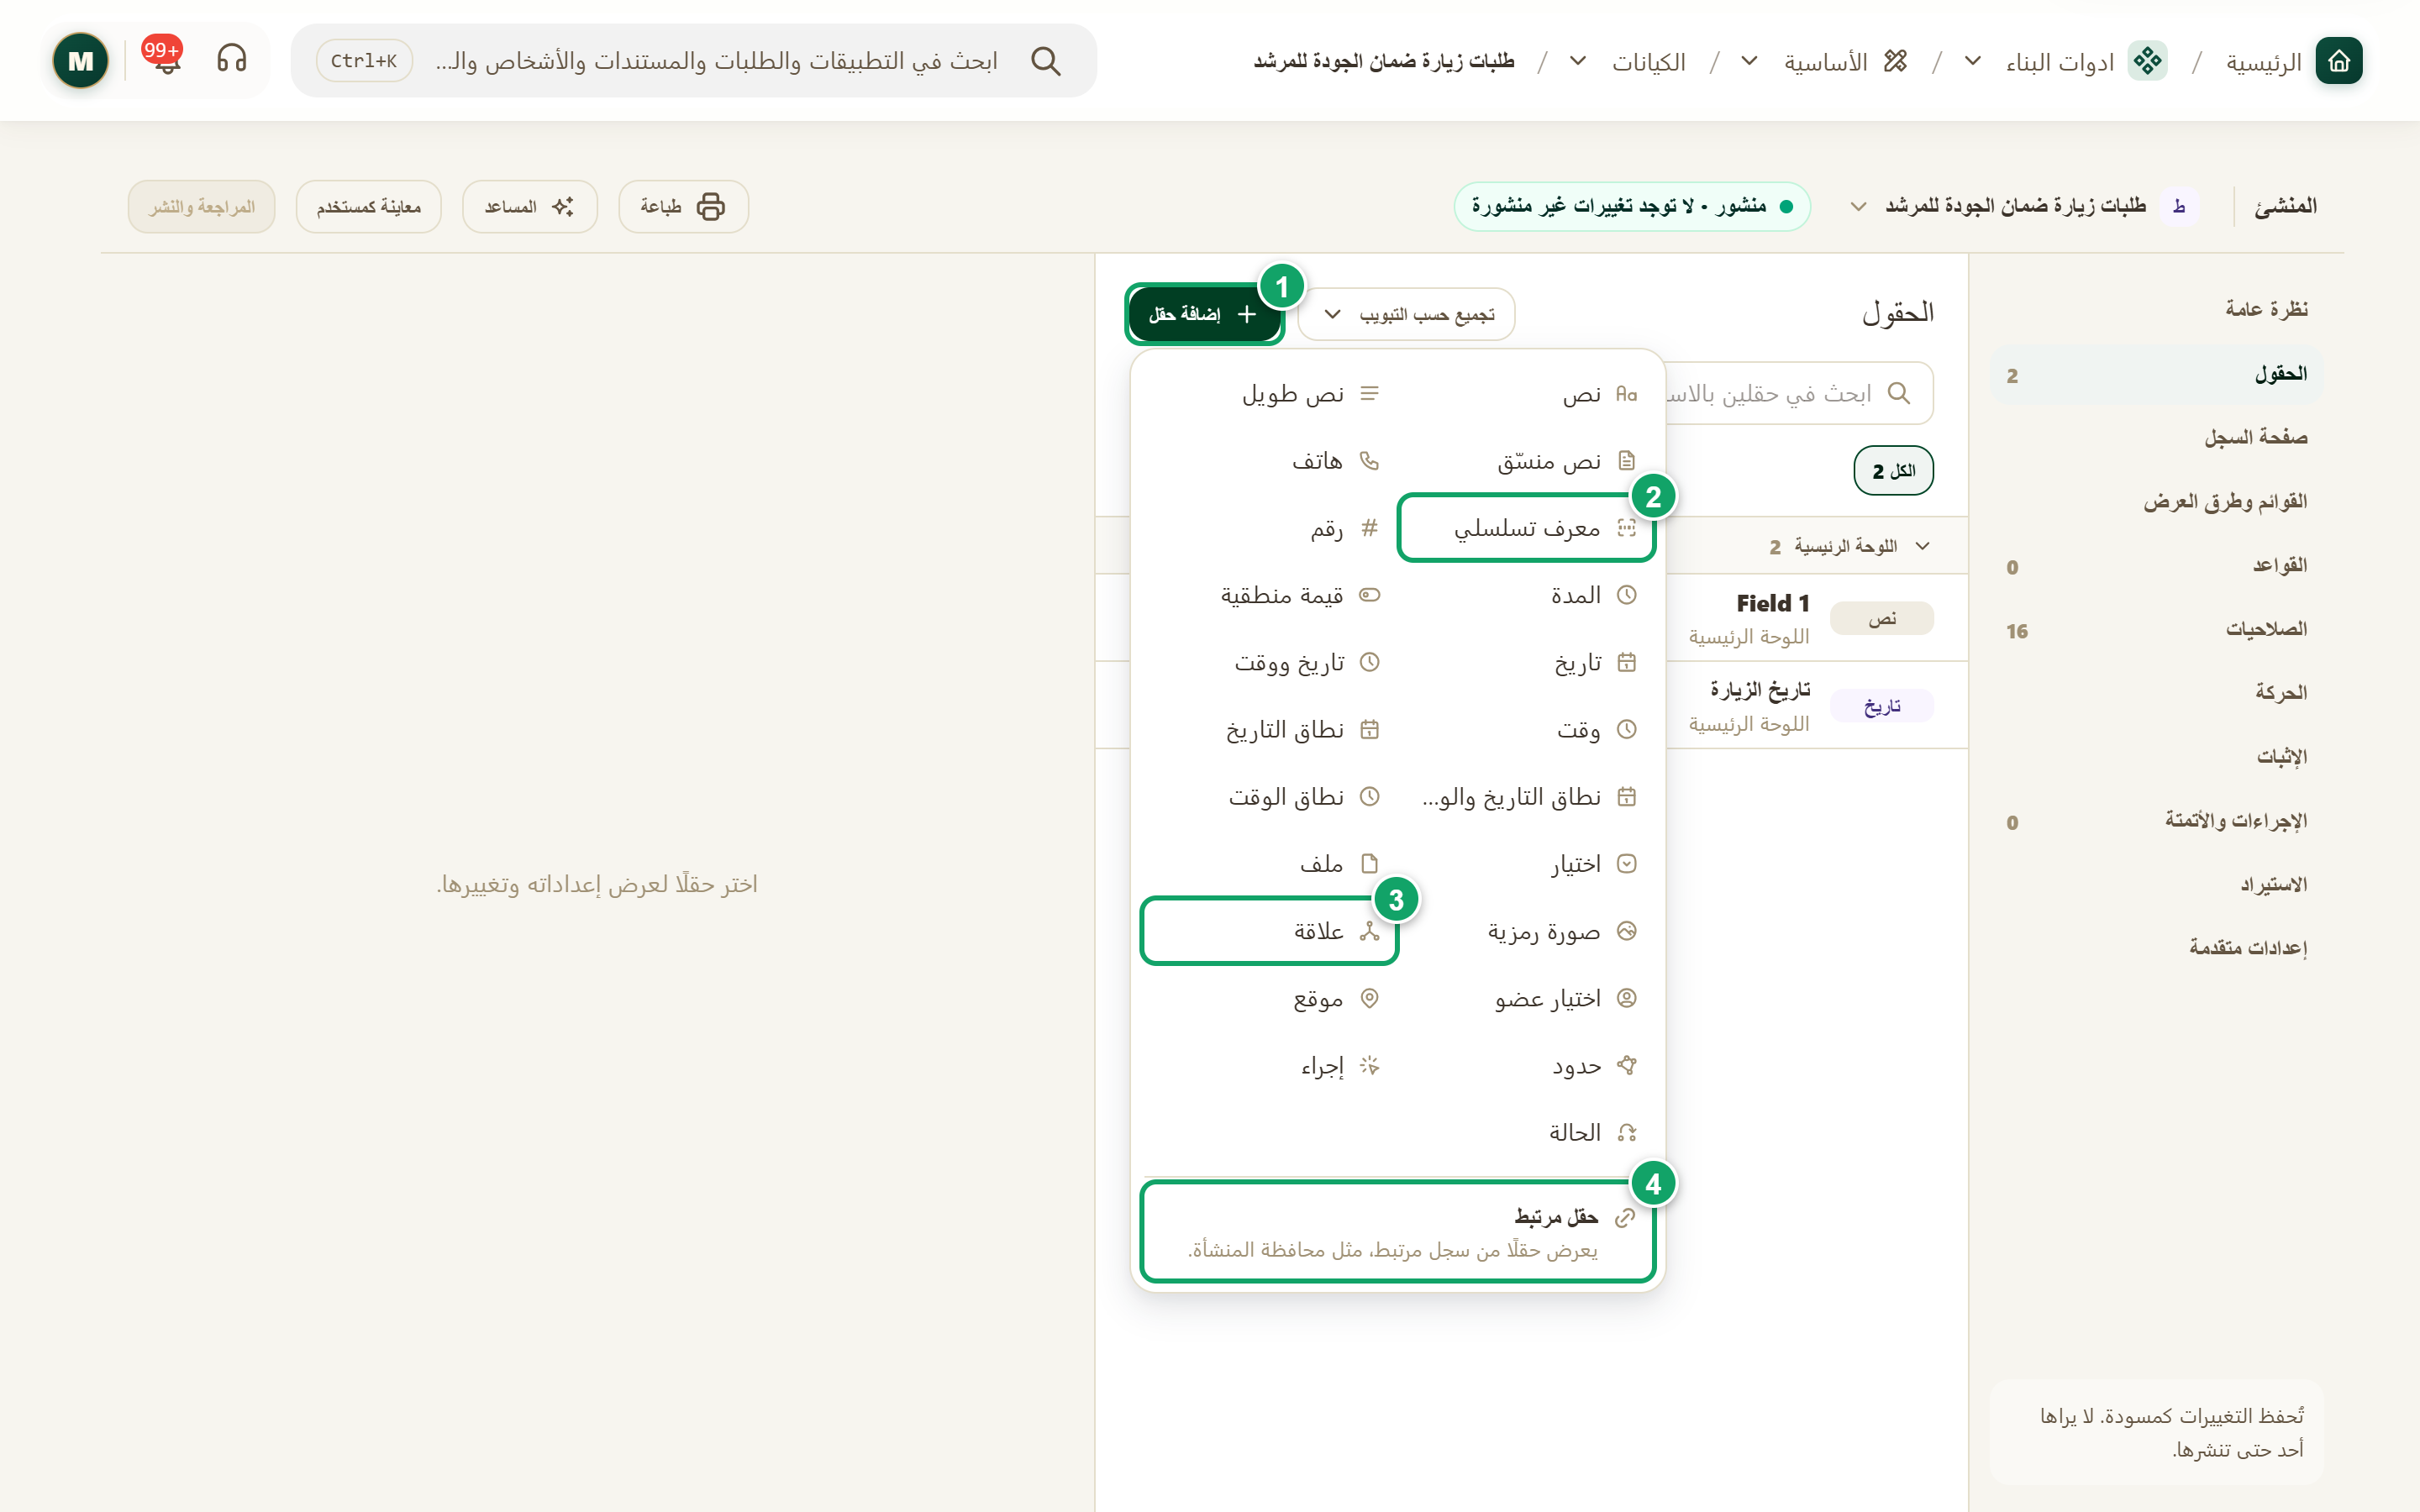
\includegraphics[width=0.95\linewidth,height=0.72\textheight,keepaspectratio]{figures/screens/ch06-ws-add-field-ar.png}
\caption{قائمة أنواع الحقول بعد الضغط على «إضافة حقل»}
\label{fig:builder-field-types-screen}
\shotnote{تعرض الصورة القائمة التي تفتح عند إضافة حقل، وفيها كل الأنواع المتاحة بالترتيب الذي تظهر به. ويفيدك ذلك في اختيار النوع الصحيح من البداية بدلاً من تغييره بعد إدخال البيانات. ① «إضافة حقل». ② «معرف تسلسلي»: لرقم مرجعي يولّده النظام. ③ «علاقة»: لربط السجل بسجل من نوع آخر. ④ «حقل مرتبط»: لعرض معلومة من سجل مرتبط.}
\end{figure}

\begin{table}[H]
\centering
\caption{الأنواع المتاحة في «إضافة حقل»}
\label{tab:builder-field-types-all}
\begin{tabularx}{\linewidth}{R{3.6cm} Y}
\rcHeaderRow
\thh{المجموعة} & \thh{الأنواع ومتى تستخدم كلاً منها}\\
النصوص & «نص» لقيمة قصيرة كالاسم، و«نص طويل» لوصف أو ملاحظة، و«نص منسّق» لنص فيه عناوين وقوائم، و«هاتف» لرقم الهاتف.\\
الأرقام والمعرّفات & «رقم» للكميات والمبالغ، و«المدة» لزمن مستغرق مثل ساعتين، و«معرف تسلسلي» لرقم مرجعي يولّده النظام لكل سجل.\\
نعم أو لا & «قيمة منطقية» لسؤال جوابه نعم أو لا، مثل «تحتاج إلى سيارة؟».\\
التواريخ والأوقات & «تاريخ» و«تاريخ ووقت» و«وقت» لقيمة واحدة، و«نطاق التاريخ» و«نطاق التاريخ والوقت» و«نطاق الوقت» لمعلومة لها بداية ونهاية.\\
الاختيار والحالة & «اختيار» لقائمة قيم ثابتة، و«الحالة» لمراحل العمل وفق قالب حالات، مثل «جديد» ثم «قيد المراجعة» ثم «معتمد».\\
الروابط والأشخاص & «علاقة» لربط السجل بسجل من نوع آخر، و«اختيار عضو» لتحديد عضو من المؤسسة، و«حقل مرتبط» لعرض معلومة من سجل مرتبط دون إعادة كتابتها.\\
الملفات والصور & «ملف» للمرفقات، و«صورة رمزية» لصورة تمثّل السجل في القوائم والبطاقات.\\
الخرائط & «موقع» لنقطة على الخريطة، و«حدود» لمساحة مرسومة على الخريطة مع مساحتها ومحيطها، مثل حدود عقار أو منشأة.\\
إجراء & زر داخل السجل يُنشئ مستند Word أو جدول Excel، أو يفتح رابطاً، أو يبدأ مسار عمل.\\
\end{tabularx}
\end{table}

\begin{table}[H]
\centering
\caption{إعدادات إضافية حسب النوع}
\label{tab:builder-field-types-settings}
\begin{tabularx}{\linewidth}{R{3.6cm} Y}
\rcHeaderRow
\thh{النوع} & \thh{ما تضبطه في «إعدادات النوع»}\\
اختيار والحالة & «الخيارات» وألوانها، و«السماح بإضافة خيارات» إذا أردت أن يضيف المستخدم قيمة جديدة، وقيمة رقمية لكل خيار عند الحاجة إلى حسابات.\\
علاقة & «مرتبط بـ» لتختار نوع السجلات الآخر، وما يحدث للسجل عند حذف السجل المرتبط: منع الحذف، أو تفريغ الحقل، أو حذف السجلات التابعة معه. وتختار في «عرض العلاقة في التبويب» و«طريقة عرض العلاقات» كيف تظهر هذه السجلات في صفحة السجل الآخر، ومن ذلك «قائمة تحقق» يُجاب عن بنودها في مكانها.\\
معرف تسلسلي & «وضع سلسلة»: «تلقائي» أو «عند الطلب» أو كلاهما، و«إدخال الرقم التسلسلي يدويًا»، و«تنسيق JEXL» الذي يحدد شكل الرقم، و«ابدأ من» و«المنطقة الزمنية».\\
الحالة & قالب الحالات الذي يحدد المراحل: «قالب ثابت» لكل السجلات، أو «قالب لكل سجل» يُختار من حقل آخر.\\
اختيار عضو & «طريقة العرض»: بيانات العضو حقولاً داخل القسم، أو تبويباً مستقلاً في صفحة السجل.\\
ملف & حدود للملفات أضيق من حدود المؤسسة، مثل أنواع الملفات المسموح بها.\\
موقع وحدود & صيغة الإحداثيات: خط العرض وخط الطول، أو \en{MGRS}، أو \en{UTM}.\\
كل الأنواع & «السماح بعدة قيم» لحفظ أكثر من قيمة في الحقل نفسه، و«نص لكل لغة» لنص يُكتب بالعربية والإنجليزية.\\
\end{tabularx}
\end{table}

\begin{figure}[H]
\centering
\begin{tikzpicture}[node distance=0.5cm]
\node[stepBox] (a) {\RL{إضافة حقل}};
\node[stepBox,below=of a] (b) {\RL{اختيار النوع المطابق}};
\node[stepBox,below=of b] (c) {\RL{إعدادات النوع}};
\node[stepBox,below=of c] (d) {\RL{قيمة واحدة أم عدة قيم}};
\node[stepBox,below=of d] (e) {\RL{تجربته في سجل}};
\draw[flowsTo] (a) -- (b);
\draw[flowsTo] (b) -- (c);
\draw[flowsTo] (c) -- (d);
\draw[flowsTo] (d) -- (e);
\end{tikzpicture}
\rclegend
\caption{اختيار نوع الحقل وضبطه}
\label{fig:builder-field-types-flow}
\shotnote{يجعل المخطط «إعدادات النوع» خطوة مستقلة لأن بعض الأنواع لا تعمل دونها: فحقل «علاقة» يحتاج إلى النوع المرتبط، و«اختيار» يحتاج إلى خياراته. أما الخطوة الأخيرة فتذكّرك بتجربة الحقل في سجل حقيقي بعد النشر، لأن شكل الإدخال لا يظهر كاملاً إلا هناك.}
\end{figure}

\subsection{خطوات العمل والتحقق}
\begin{enumerate}
\item في «الحقول» اضغط «إضافة حقل»، واختر النوع الذي يطابق المعلومة لا شكلها؛ فرقم الهاتف «هاتف» وليس «رقم».
\item افتح «إعدادات النوع» وأكمل ما يطلبه النوع: الخيارات في «اختيار»، والنوع المرتبط في «علاقة»، والتنسيق في «معرف تسلسلي».
\item فعّل «السماح بعدة قيم» فقط إذا كان السجل الواحد يحتاج فعلاً إلى أكثر من قيمة، مثل عدة مرفقات.
\item انشر التغييرات، ثم أنشئ سجلاً تجريبياً وأدخل قيمة في الحقل الجديد.
\end{enumerate}

\textbf{تحقق ومعالجة المشكلة:} يجب أن يقبل الحقل القيمة الصحيحة بالشكل المتوقع، مثل منتقي التاريخ في حقل «تاريخ». فإذا ظهر في «قبل النشر» خطأ عن خيارات فارغة أو مكررة، فافتح «الخيارات» وأكمل القيم أو احذف المكرر منها.

\clearpage
\section{مصدر القيمة: الحقول المحسوبة والمرتبطة والمجمّعة}
\label{sec:builder-feature-field-values}

لا يكتب المستخدم كل قيمة بنفسه؛ فبعض القيم تُحسب من حقول السجل، أو تُنقل من سجل مرتبط، أو تُجمع من السجلات التي ترتبط به. ويحدد إعداد «مصدر القيمة» في لوحة الحقل من أين تأتي القيمة، فتقلّ الأخطاء ولا تتكرر المعلومة في أكثر من مكان. وتشرح هذه الصفحة أيضاً إعداد «إلزامي» لأنه يتعلق بطريقة الحصول على القيمة.

\textbf{المسار ومن يستخدمه:} «المنشئ» ← «الحقول» ← اختر الحقل ← «القيمة» ← «مصدر القيمة». يستخدمه من يبني النوع. ولا يظهر هذا الإعداد في حقول «إجراء» و«الحالة» و«معرف تسلسلي».

\begin{rcnote}[مثال: شركة الأفق]
يضيف المسؤول إلى «طلبات الزيارة» حقل «محافظة الفرع» مصدره «من سجل مرتبط»، فيأخذ المحافظة من سجل الفرع تلقائياً. ويضيف إلى نوع الفروع حقل «عدد الزيارات» مصدره «مجمّعة»، يعدّ طلبات الزيارة المرتبطة بكل فرع.
\end{rcnote}

\begin{figure}[H]
\centering
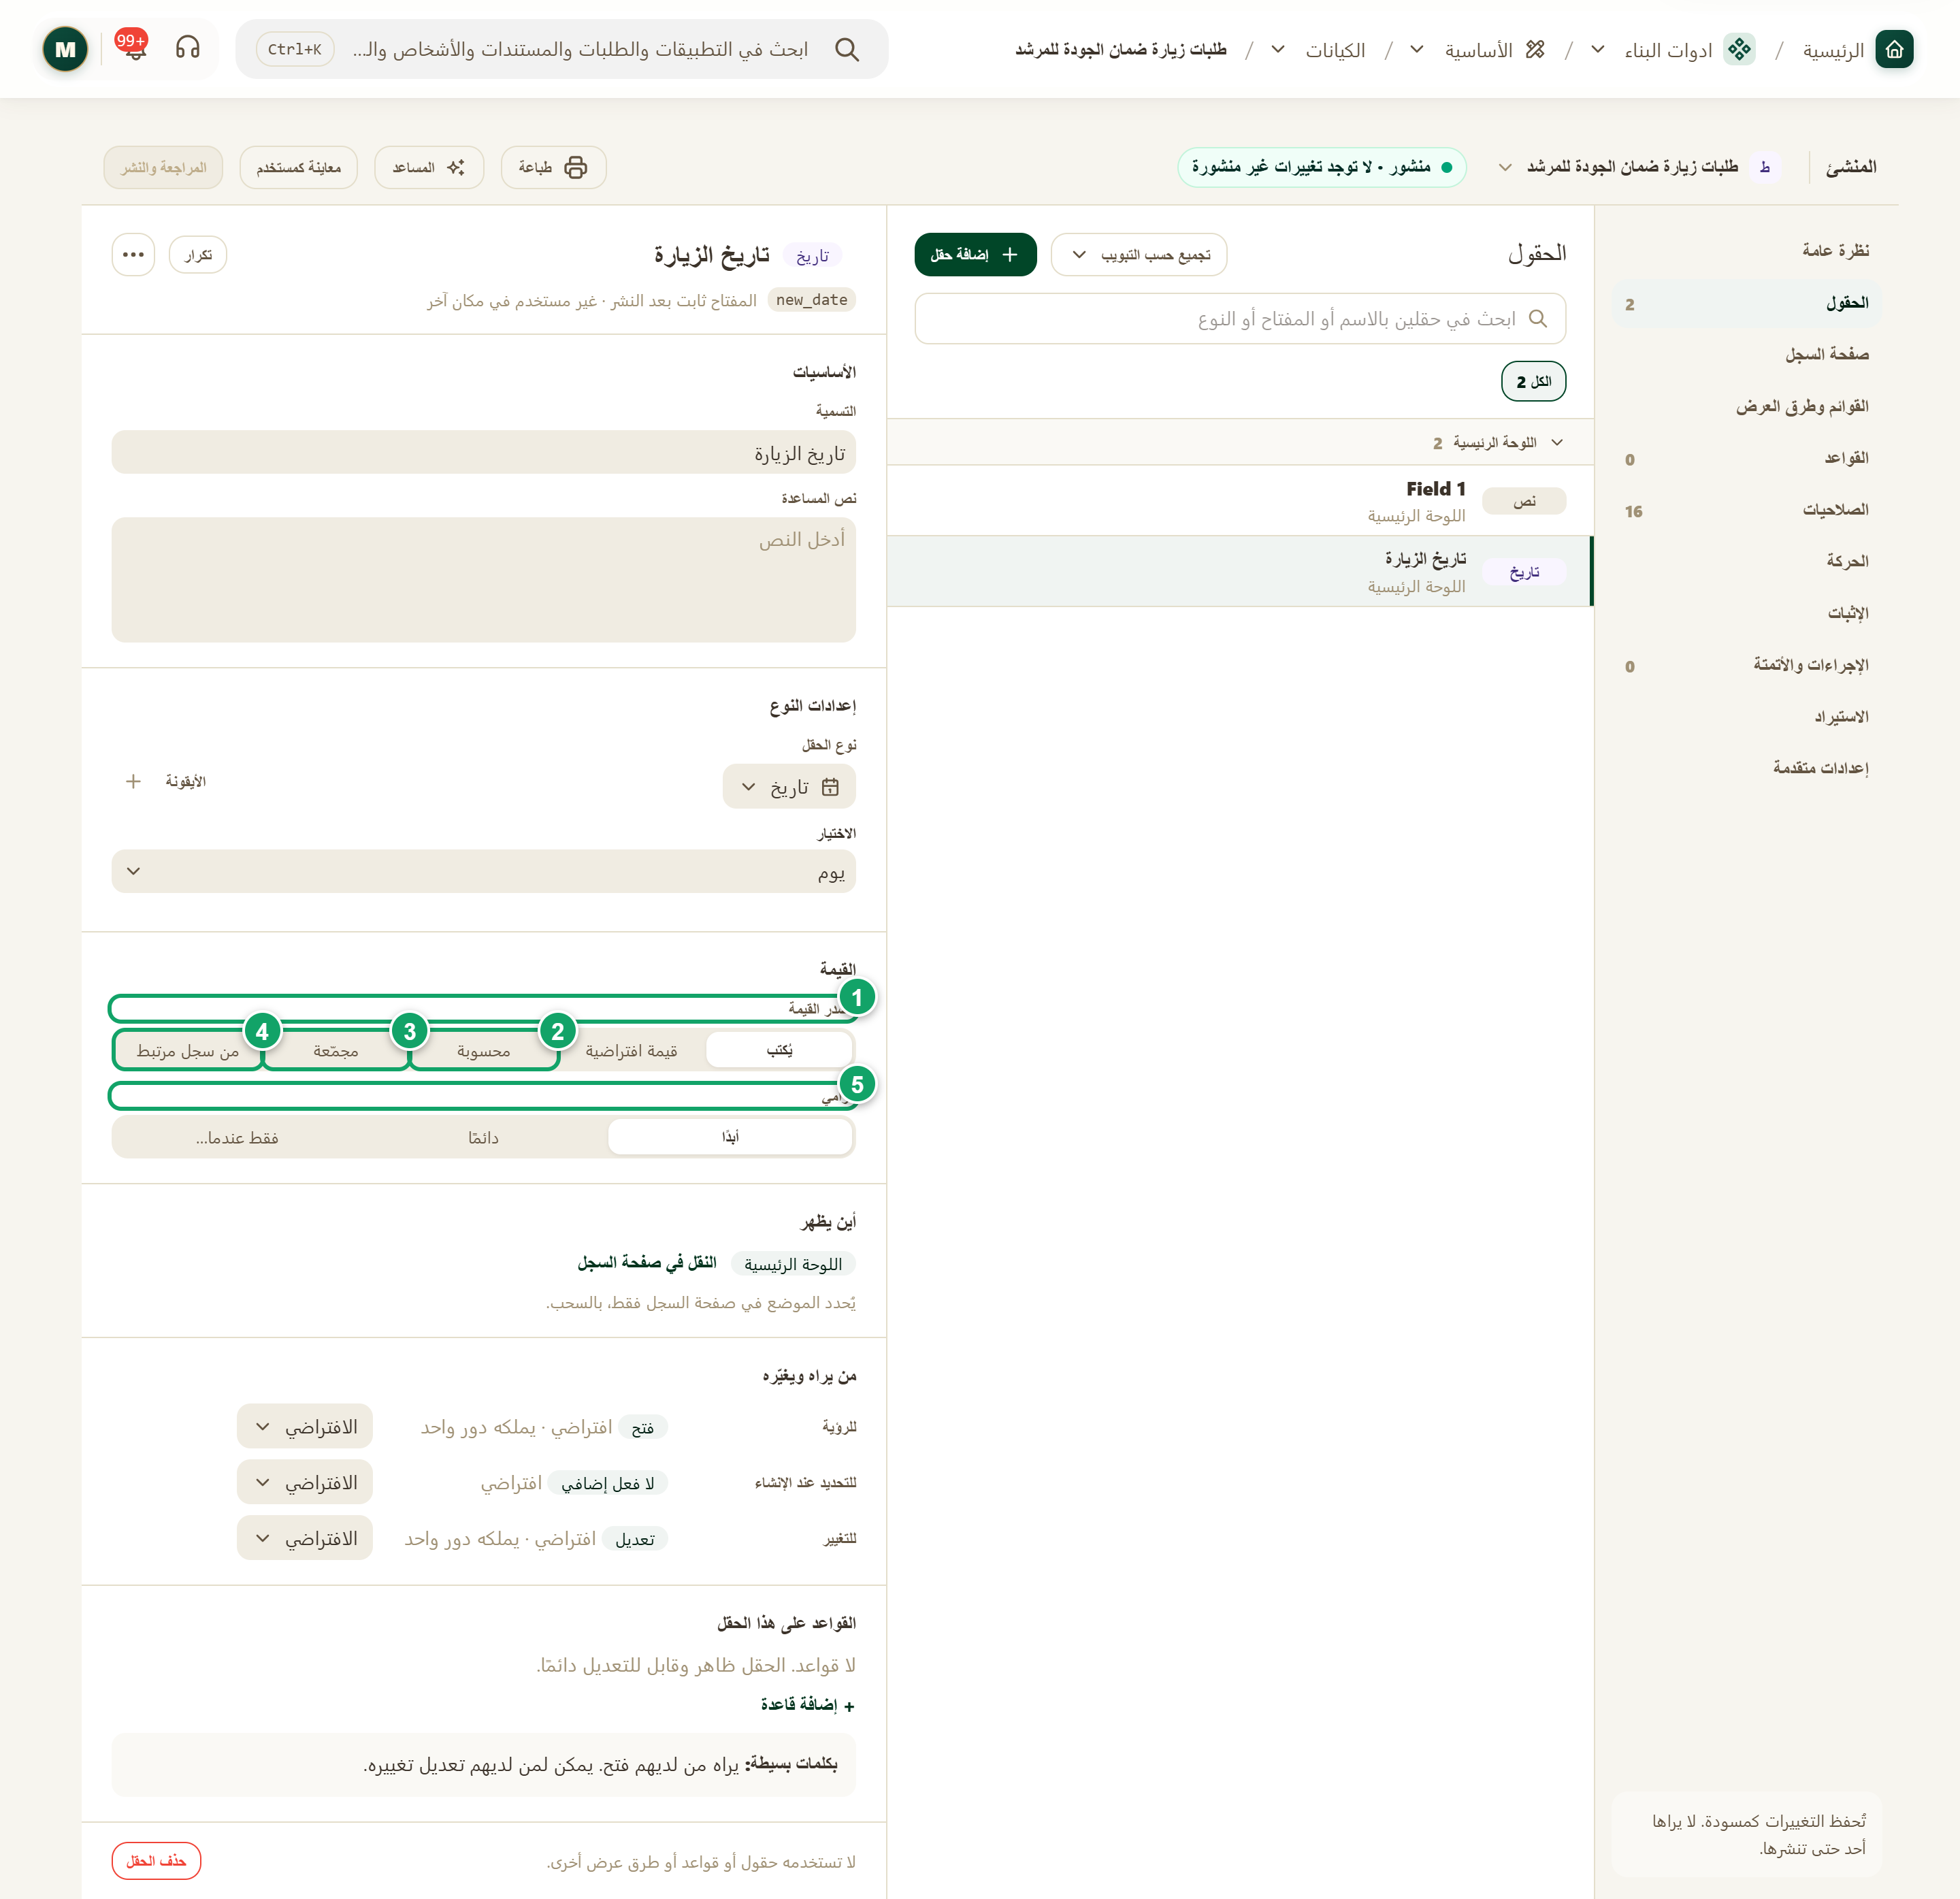
\includegraphics[width=0.95\linewidth,height=0.72\textheight,keepaspectratio]{figures/screens/ch06-ws-value-source-ar.png}
\caption{إعداد «مصدر القيمة» في لوحة حقل تاريخ}
\label{fig:builder-field-values-screen}
\shotnote{تعرض الصورة إعدادات حقل «تاريخ الزيارة» في النوع الاختباري، وقد ظهر فيها قسم «القيمة» بخياراته. ويبيّن ذلك أن مصدر القيمة وإلزامها يُضبطان في مكان واحد من لوحة الحقل. ① «مصدر القيمة». ② «محسوبة»: القيمة ناتج صيغة. ③ «مجمّعة»: القيمة من السجلات المرتبطة. ④ «من سجل مرتبط»: القيمة من حقل في سجل مرتبط. ⑤ «إلزامي»: متى يُمنع الحفظ إذا بقي الحقل فارغاً.}
\end{figure}

\begin{table}[H]
\centering
\caption{خيارات «مصدر القيمة»}
\label{tab:builder-field-values-sources}
\begin{tabularx}{\linewidth}{R{3.6cm} Y}
\rcHeaderRow
\thh{الخيار} & \thh{متى تستخدمه}\\
يُكتب & يكتب المستخدم القيمة بنفسه. وهو الخيار المعتاد لمعظم الحقول.\\
قيمة افتراضية & تبدأ القيمة بقيمة تحددها، ويستطيع المستخدم تغييرها، مثل حالة أولية أو تاريخ اليوم.\\
محسوبة & تُحسب القيمة بصيغة من حقول السجل نفسه أو السجلات المرتبطة به، مثل الكمية مضروبة في السعر. وتحدد في «التحديث التلقائي» هل تُعاد الحسبة عند تغيّر بيانات السجل فقط أم يومياً أو أسبوعياً أو شهرياً.\\
مجمّعة & تُجمع القيمة من السجلات التي ترتبط بهذا السجل أو من المهام المرتبطة به: عددها، أو مجموع حقل فيها، أو متوسطه، أو أقله أو أعلاه، أو أقدم تاريخ وأحدثه.\\
من سجل مرتبط & تُعرض قيمة حقل من سجل مرتبط، مثل محافظة الفرع، وتتحدث تلقائياً عند تغيّرها هناك.\\
\end{tabularx}
\end{table}

\subsection{بناء قيمة مجمّعة}

عندما تختار «مجمّعة» يظهر محرر يقودك خطوة بخطوة. تبدأ بـ«التجميع من» فتختار السجلات التي ترتبط بهذا السجل، ثم تختار في «الحساب» العملية، مثل «العدد» أو «المجموع» أو «المتوسط». وتستطيع أن تضيّق السجلات بشروط في «تضمين السجلات التي»، وأن تقسم النتيجة على عدد السجلات لتعرضها نسبة مئوية. وتعرض المعاينة النتيجة على سجل نموذجي، ثم تضغط «استخدام هذا التجميع».

\subsection{عرض قيمة من سجل مرتبط}

عندما تختار «من سجل مرتبط» تظهر نافذة «من أين تأتي القيمة؟»، فتختار العلاقة ثم الحقل الذي تريد عرضه. وإذا كان للسجل أكثر من سجل مرتبط، فتحدد في «الحساب» هل تعرض أولها أو قائمة بقيمها أو عددها أو مجموعها. وتحدد أيضاً ما يظهر عندما لا يوجد سجل مرتبط: حقل فارغ أو نص تكتبه. ولا تُحسب السجلات المؤرشفة، ولا يمكن جعل هذا الحقل إلزامياً؛ فاجعل حقل العلاقة نفسه إلزامياً بدلاً منه.

\subsection{إلزامي: أبدًا أو دائمًا أو فقط عندما}

يحدد إعداد «إلزامي» متى يُمنع حفظ السجل إذا بقي الحقل فارغاً: «أبدًا»، أو «دائمًا»، أو «فقط عندما…» لحالة معينة. والخيار الأخير ينقلك إلى «القواعد» لتبني قاعدة «إلزام» بشرطها. ولا يتاح هذا الإعداد في الحقول المحسوبة والمرتبطة، لأن المستخدم لا يكتب قيمتها.

\begin{figure}[H]
\centering
\begin{tikzpicture}[node distance=0.5cm]
\node[stepBox] (a) {\RL{اختيار مجمّعة}};
\node[stepBox,below=of a] (b) {\RL{التجميع من}};
\node[stepBox,below=of b] (c) {\RL{الحساب}};
\node[stepBox,below=of c] (d) {\RL{تضمين السجلات التي}};
\node[stepBox,below=of d] (e) {\RL{المعاينة على سجل}};
\node[stepBox,below=of e] (f) {\RL{استخدام هذا التجميع}};
\draw[flowsTo] (a) -- (b);
\draw[flowsTo] (b) -- (c);
\draw[flowsTo] (c) -- (d);
\draw[flowsTo] (d) -- (e);
\draw[flowsTo] (e) -- (f);
\end{tikzpicture}
\rclegend
\caption{بناء قيمة مجمّعة}
\label{fig:builder-field-values-flow}
\shotnote{يتبع المخطط ترتيب المحرر نفسه: تختار السجلات أولاً لأن العمليات المتاحة تعتمد على حقولها، ثم الحساب، ثم الشروط التي تضيّقها. وتأتي المعاينة قبل الحفظ لترى الرقم على سجل حقيقي، فتكتشف خطأ الشرط أو العملية قبل أن يراه الفريق.}
\end{figure}

\subsection{خطوات العمل والتحقق}
\begin{enumerate}
\item أضف حقلاً من النوع المناسب للنتيجة، مثل «رقم» للعدد أو المجموع، ثم افتح «القيمة» واختر «مصدر القيمة».
\item لقيمة محسوبة، اختر «محسوبة» واكتب الصيغة في المحرر، ثم اختر «التحديث التلقائي» المناسب.
\item لقيمة مجمّعة، اتبع المحرر من «التجميع من» إلى «استخدام هذا التجميع».
\item لقيمة من سجل مرتبط، تأكد أن حقل «علاقة» موجود، ثم اختر «من سجل مرتبط» وحدد العلاقة والحقل.
\item انشر التغييرات، ثم افتح سجلاً مرتبطاً بسجلات أخرى وقارن القيمة بما تتوقعه.
\end{enumerate}

\textbf{تحقق ومعالجة المشكلة:} يجب أن تظهر القيمة دون أن يكتبها أحد، وأن تتغير عندما تتغير مصادرها. فإذا ظهر في «قبل النشر» «لا يمكن حساب» متبوعاً باسم الحقل، فالصيغة تشير إلى حقل غير موجود؛ اضغط «إصلاح المعادلة» واختر الحقل الصحيح. وإذا اخترت «يُكتب» لحقل مرتبط، فستبقى قيمه الحالية لكنها لن تتحدث بعد ذلك.

\clearpage
\section{حقل الحالة وقواعد دورة الحياة}
\label{sec:builder-feature-lifecycle}

حقل «الحالة» يتبع مراحل العمل في قالب حالات، مثل «جديد» ثم «قيد المراجعة» ثم «معتمد». وتضيف إليه «قواعد دورة الحياة» ضوابط: متى يُسمح بالانتقال من حالة إلى أخرى، ومن لا يحق له تنفيذه، وما الحقول التي تُضبط تلقائياً عند الانتقال، وهل يُقفل السجل في حالة معينة. فلا يعتمد الالتزام بالإجراء على تذكّر الموظفين.

\textbf{المسار ومن يستخدمه:} «المنشئ» ← «الحقول» ← اختر حقل الحالة ← «قواعد دورة الحياة». تحتاج القواعد إلى «قالب ثابت» في إعدادات الحقل، ولا تتاح في أنواع السجلات المدمجة. أما قوالب الحالات نفسها فيشرحها فصل المهام في الصفحة \ref{sec:tasks-feature-statuses}.

\begin{rcnote}[مثال: شركة الأفق]
يجعل المسؤول الانتقال إلى «معتمد» في «طلبات الزيارة» ممنوعاً على مقدّم الطلب نفسه، فلا يعتمد عمر حداد طلبه. ويضيف أثراً يكتب تاريخ الاعتماد واسم من اعتمد، ثم يقفل الطلب المعتمد فلا تتغير بياناته بعد أن تعتمده سارة الخطيب.
\end{rcnote}

\begin{table}[H]
\centering
\caption{ما تضبطه لكل انتقال}
\label{tab:builder-lifecycle-transitions}
\begin{tabularx}{\linewidth}{R{3.6cm} Y}
\rcHeaderRow
\thh{الإعداد} & \thh{المعنى}\\
فقط عندما & شرط يجب أن يتحقق قبل الانتقال، مثل وجود تاريخ للزيارة.\\
الرسالة عند المنع & النص الذي يراه المستخدم إذا لم يتحقق الشرط، فيعرف ما ينقصه.\\
لا يمكن أن ينفّذه الأعضاء المذكورون في & حقول أعضاء في السجل لا يحق لأصحابها تنفيذ الانتقال، مثل مقدّم الطلب.\\
عند تنفيذ الانتقال & آثار تُضبط في الحفظ نفسه: «اضبط» حقلاً على «الآن» أو «العضو الحالي» أو قيمة ثابتة أو تعبير، أو «امسح» قيمته. وتُكتب هذه الحقول حتى لو كان السجل مقفلاً.\\
\end{tabularx}
\end{table}

\begin{table}[H]
\centering
\caption{ما تضبطه لكل حالة}
\label{tab:builder-lifecycle-states}
\begin{tabularx}{\linewidth}{R{3.6cm} Y}
\rcHeaderRow
\thh{الإعداد} & \thh{المعنى}\\
التعديل & «غير مقفل»، أو «مقفل»، أو «مقفل باستثناء» حقول تبقى قابلة للتعديل.\\
منع الحذف & يمنع حذف السجل ما دام في هذه الحالة.\\
قفل السجلات التي تشير إليه & يقفل أيضاً السجلات المرتبطة به، مثل بنود طلب معتمد.\\
تجميد إصدار عند الدخول & يحفظ نسخة من السجل باسم تحدده عند دخوله الحالة، لتعود إليها لاحقاً.\\
\end{tabularx}
\end{table}

\begin{rcwarn}[الحالة تتغير بالانتقالات فقط]
عند تفعيل «لا تتغير الحالة إلا عبر الانتقالات» لا تستطيع النماذج أو الاستيراد أو الأتمتة أن تضبط الحالة مباشرة، ويبدأ كل سجل جديد من الحالة الأولى. فإذا كانت لديك أتمتة تغيّر الحالة، فراجعها قبل تفعيل هذا الخيار.
\end{rcwarn}

\begin{figure}[H]
\centering
\begin{tikzpicture}[node distance=0.5cm]
\node[stepBox] (a) {\RL{قالب ثابت للحالة}};
\node[stepBox,below=of a] (b) {\RL{شروط الانتقالات}};
\node[stepBox,below=of b] (c) {\RL{من لا ينفّذ الانتقال}};
\node[stepBox,below=of c] (d) {\RL{آثار الانتقال}};
\node[stepBox,below=of d] (e) {\RL{القفل في كل حالة}};
\draw[flowsTo] (a) -- (b);
\draw[flowsTo] (b) -- (c);
\draw[flowsTo] (c) -- (d);
\draw[flowsTo] (d) -- (e);
\end{tikzpicture}
\rclegend
\caption{ضبط دورة حياة السجل}
\label{fig:builder-lifecycle-flow}
\shotnote{يبدأ المخطط بالقالب الثابت لأن القواعد كلها تُبنى على انتقالاته، فلا تظهر دونه. ثم يضبط كل انتقال على حدة، وينتهي بالقفل لأنه يحمي السجل بعد وصوله إلى الحالة، فيصبح الترتيب: متى ينتقل السجل، ومن ينقله، وماذا يحدث بعد ذلك.}
\end{figure}

\subsection{خطوات العمل والتحقق}
\begin{enumerate}
\item افتح حقل الحالة في «الحقول»، واختر في «إعدادات النوع» «قالب ثابت» وقالب الحالات المناسب.
\item افتح «قواعد دورة الحياة»، واختر الانتقال الذي تريد ضبطه، وأضف شرطه في «فقط عندما» ورسالته في «الرسالة عند المنع».
\item حدد في «لا يمكن أن ينفّذه الأعضاء المذكورون في» حقل مقدّم الطلب إن كان لا يحق له اعتماد طلبه.
\item أضف في «عند تنفيذ الانتقال» أثراً يكتب التاريخ أو العضو الحالي، ثم حدد قفل التعديل للحالة النهائية.
\item انشر التغييرات، وجرّب الانتقال بسجل تجريبي مرة بشرط ناقص ومرة بشرط مكتمل.
\end{enumerate}

\textbf{تحقق ومعالجة المشكلة:} يجب أن يُمنع الانتقال مع رسالتك عندما ينقص الشرط، وأن يتم ويكتب الحقول المحددة عندما يكتمل. فإذا لم تظهر «قواعد دورة الحياة»، فاختر «قالب ثابت» أولاً؛ وإذا كان النوع مدمجاً في النظام، فهذه القواعد غير متاحة له.

\clearpage
\section{صفحة السجل}
\label{sec:builder-feature-record-page}

صفحة السجل هي ما يراه المستخدم عندما يفتح سجلاً واحداً. ويرتّب قسم «صفحة السجل» الحقول في تبويبات وأقسام، فتظهر المعلومات المترابطة معاً بدلاً من قائمة طويلة واحدة. ويمكنك أن تضيف كتلاً في أعلى التبويب الأول، وقوائم بالسجلات المرتبطة.

\textbf{المسار ومن يستخدمه:} نوع السجلات ← «صفحة السجل». يستخدمه من يبني النوع بعد إضافة حقوله.

\begin{rcnote}[مثال: شركة الأفق]
يجعل مسؤول النظام لصفحة طلب الزيارة تبويبين: «الطلب» للفرع والموعد والغرض، و«المراجعة» لملاحظات سارة الخطيب وقرارها، فيجد عمر حداد ما يخصه في التبويب الأول. ويبدأ بإنشاء التبويبين من ② ثم يسحب الحقول إليهما.
\end{rcnote}

\begin{figure}[H]
\centering
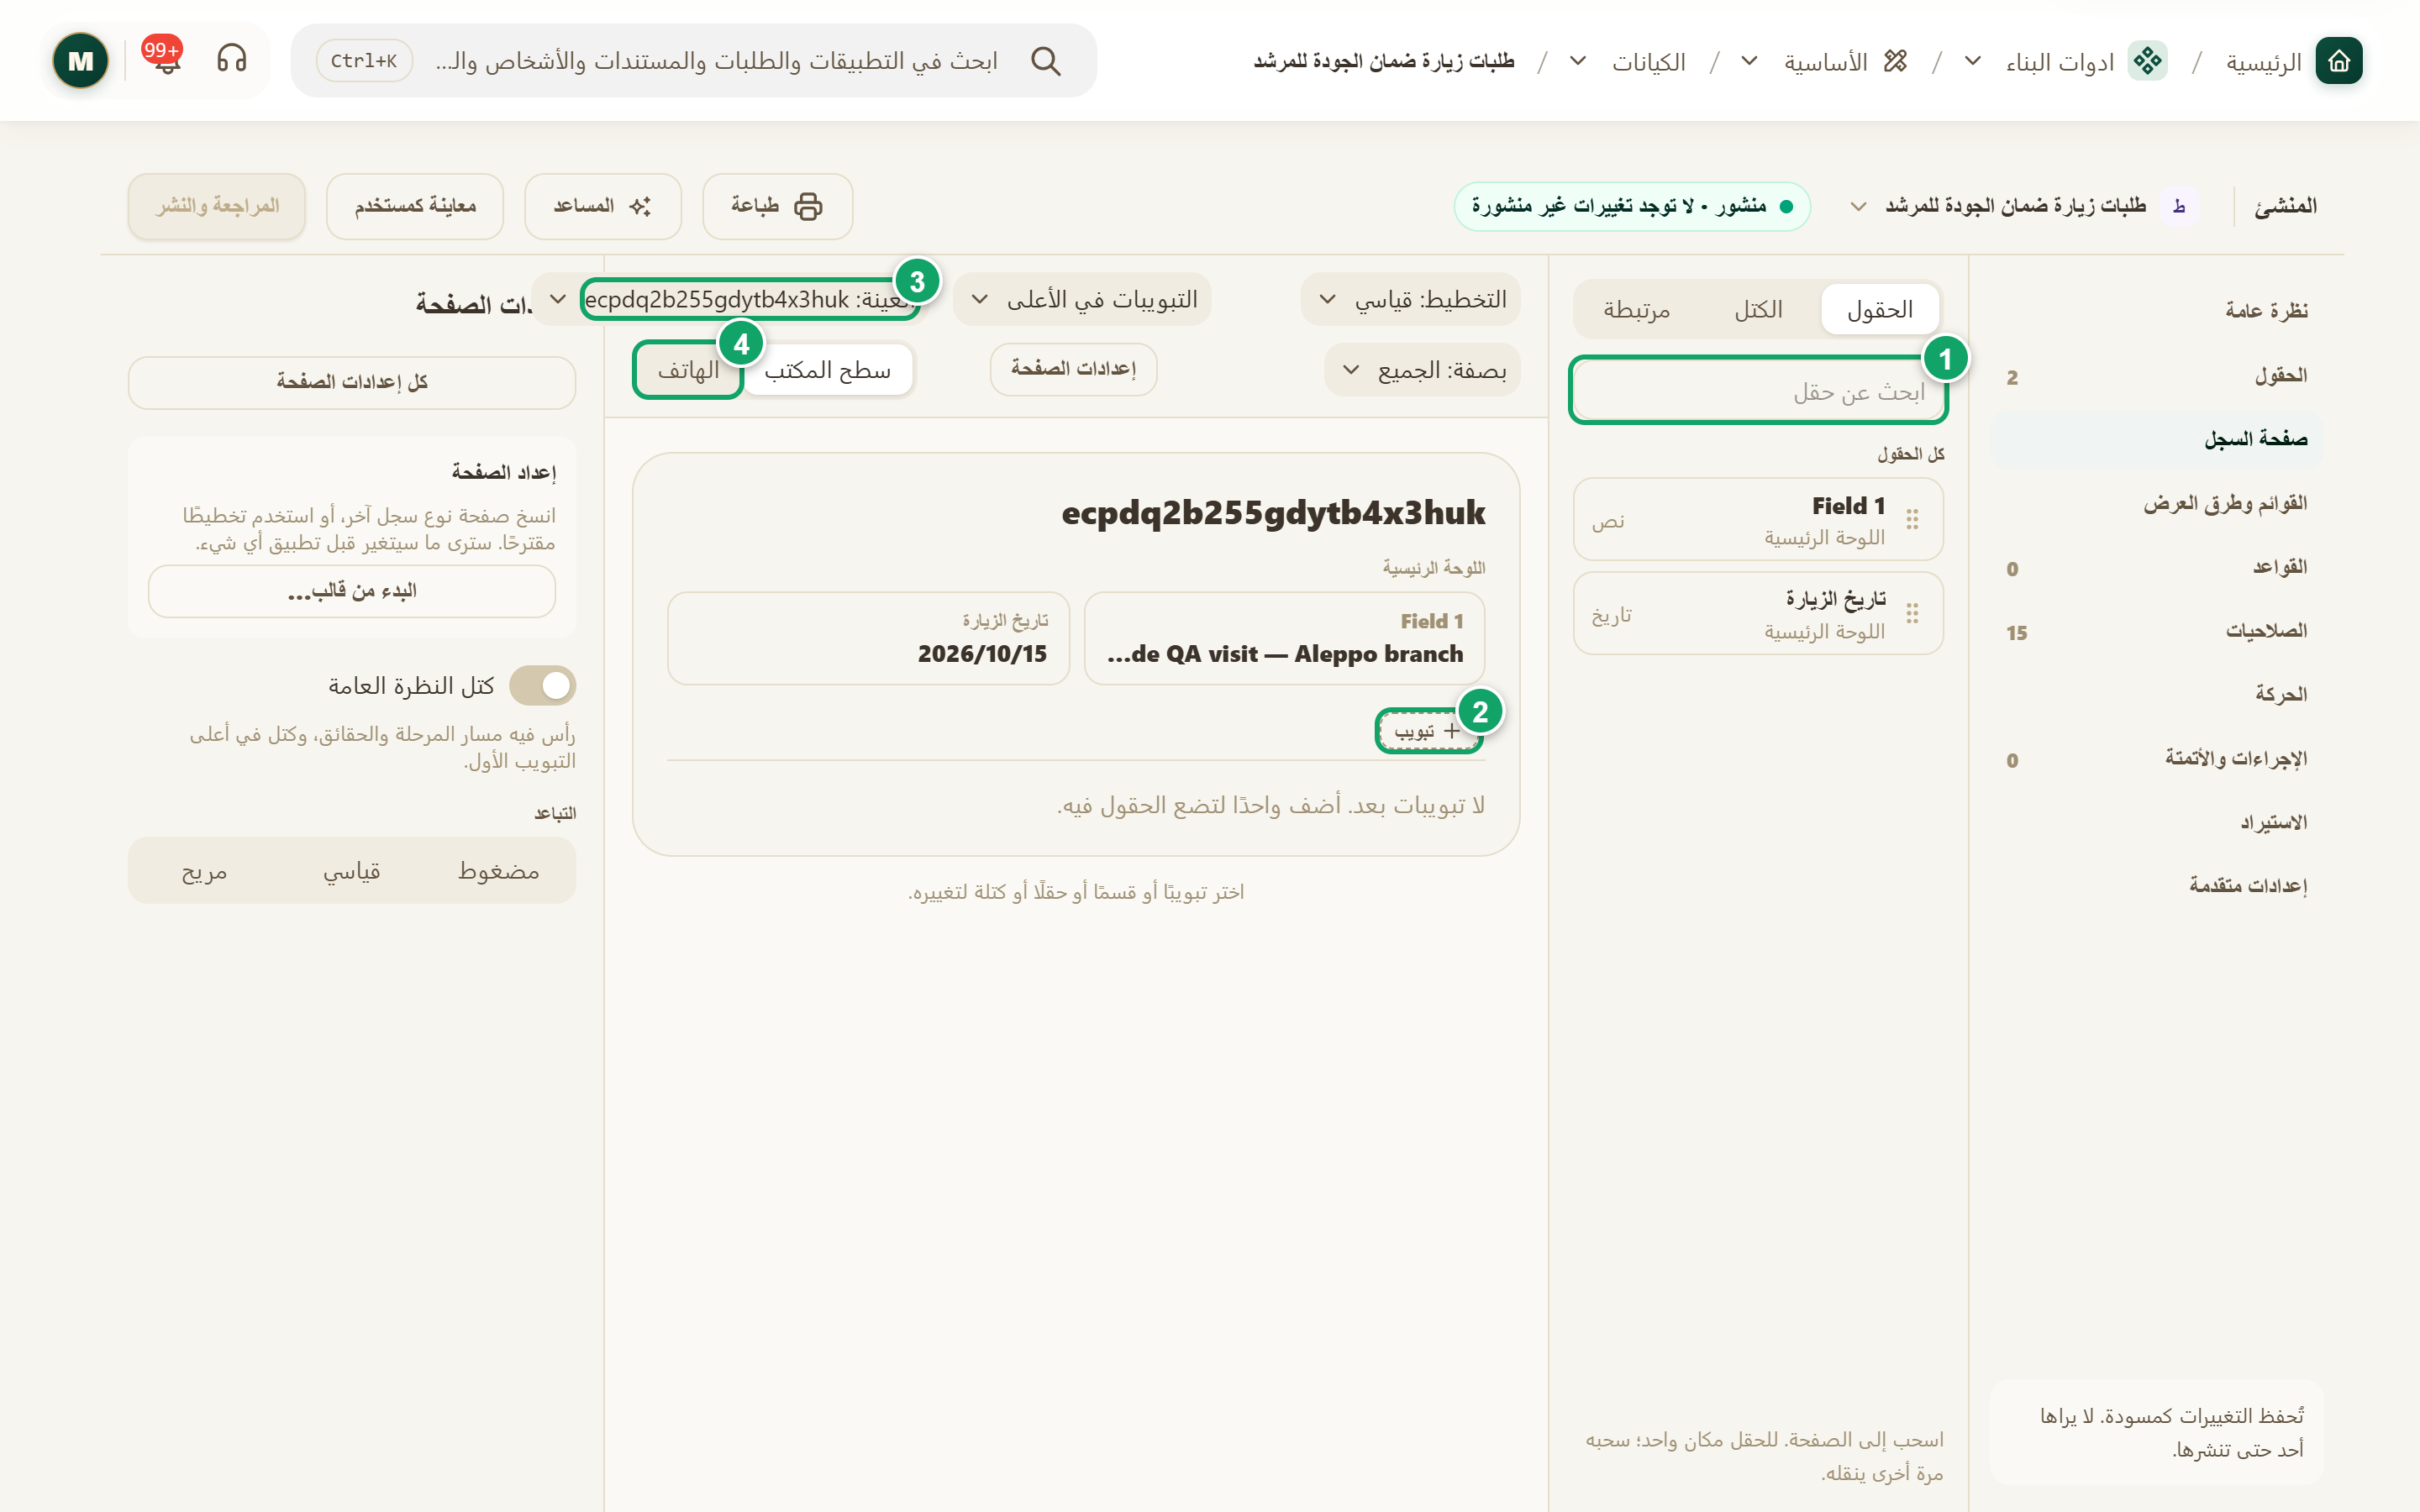
\includegraphics[width=0.95\linewidth,height=0.72\textheight,keepaspectratio]{figures/screens/ch06-ws-record-page-ar.png}
\caption{قسم «صفحة السجل» مع معاينة بسجل حقيقي}
\label{fig:builder-record-page-screen}
\shotnote{يعرض القسم أجزاء الصفحة على جانب، والصفحة نفسها في الوسط بقيم سجل اختباري، فترى أثر الترتيب قبل النشر. ① «ابحث عن حقل»: تجد الحقل الذي تريد سحبه إلى الصفحة. ② «تبويب»: يضيف تبويباً تضع فيه الأقسام والحقول. ③ «العينة»: السجل الذي تُعاين به الصفحة. ④ «الهاتف»: يعرض الصفحة كما تظهر على الشاشة الصغيرة.}
\end{figure}


\begin{table}[H]
\centering
\caption{ما الذي تجده هنا؟}
\label{tab:builder-record-page-data}
\begin{tabularx}{\linewidth}{R{3.6cm} Y}
\rcHeaderRow
\thh{القسم} & \thh{المحتوى والإجراء}\\
التبويبات والأقسام & أنشئ «تبويب جديد» أو «قسم جديد»، ثم اسحب الحقول إليها. للحقل مكان واحد في الصفحة، وسحبه مرة أخرى ينقله.\\
أجزاء الصفحة & تجمع «كل الحقول» و«الكتل» والقوائم «المرتبطة»، وتعرض الحقول التي «ليست في الصفحة بعد».\\
التخطيط والرأس & يختار شكل الصفحة: تبويبات أو قائمة أقسام، مع إعدادات الرأس وكتل النظرة العامة.\\
المعاينة & تعرض الصفحة بعينة من سجل حقيقي، كما يراها دور معيّن، على سطح المكتب أو الهاتف.\\
\end{tabularx}
\end{table}

\begin{figure}[H]
\centering
\begin{tikzpicture}[node distance=0.5cm]
\node[entity] (page) {\RL{صفحة السجل}};
\node[entity,below=0.7cm of page] (tab) {\RL{تبويب}};
\node[entity,below=0.7cm of tab] (section) {\RL{قسم}};
\node[entity,below=0.7cm of section] (field) {\RL{حقل}};
\draw[dependsOn] (page) -- (tab);
\draw[dependsOn] (tab) -- (section);
\draw[dependsOn] (section) -- (field);
\end{tikzpicture}
\rclegend
\caption{كيف تُرتّب الصفحة}
\label{fig:builder-record-page-tree}
\shotnote{يوضّح الشكل تدرّج الترتيب: تضم الصفحة تبويبات، ويضم كل تبويب أقساماً، ويضم كل قسم حقولاً. لذلك تنشئ التبويب والقسم أولاً ثم تسحب الحقول إليهما، والحقل الذي لا تضعه في أي قسم يبقى محفوظاً لكنه لا يظهر في الصفحة.}
\end{figure}

\subsection{خطوات العمل والتحقق}
\begin{enumerate}
\item افتح نوع السجلات واختر «صفحة السجل».
\item أنشئ التبويبات التي يحتاجها العمل، ثم أضف قسماً أو أكثر في كل تبويب.
\item اسحب كل حقل من «أجزاء الصفحة» إلى القسم المناسب، وراجع «ليست في الصفحة بعد» حتى لا يبقى حقل مهم خارج الصفحة.
\item غيّر حجم المعاينة إلى «الهاتف» لتتأكد من أن الصفحة واضحة على الشاشة الصغيرة.
\end{enumerate}

\textbf{تحقق ومعالجة المشكلة:} يجب أن تعرض المعاينة الحقول في التبويبات والأقسام التي اخترتها. فإذا لم يظهر حقل، فابحث عنه في «ليست في الصفحة بعد» واسحبه إلى قسم؛ وإذا ظهرت رسالة بأن الحقل موضوع في تبويب غير موجود، فانقله إلى تبويب قائم.

\clearpage
\section{كتل النظرة العامة والتخطيطات}
\label{sec:builder-feature-record-page-blocks}

إلى جانب الحقول، يمكن أن تبدأ صفحة السجل بملخص يعرض أهم ما فيه: مسار المراحل، وأرقام رئيسية، وما يحتاج إلى متابعة. وتُبنى هذه الملخصات من «كتل النظرة العامة» التي تظهر أعلى التبويب الأول. أما «التخطيطات» فنسخ محفوظة من ترتيب الصفحة، تختار بينها حسب قيمة في السجل، فيرى كل نوع من السجلات الترتيب الأنسب له.

\textbf{المسار ومن يستخدمه:} «المنشئ» ← «صفحة السجل» ← «إعدادات الصفحة» لتفعيل كتل النظرة العامة، ثم «أجزاء الصفحة» ← «الكتل» لإضافتها. والتخطيطات من «إدارة التخطيطات…». يستخدمه من يبني النوع بعد أن تستقر حقوله.

\begin{rcnote}[مثال: شركة الأفق]
يضيف المسؤول إلى صفحة «طلبات الزيارة» كتلة «مؤشرات» تعرض عدد أيام الطلب منذ إنشائه، وكتلة «يحتاج إلى متابعة» تنبّه سارة الخطيب إلى الطلب الذي مضى عليه أكثر من ثلاثة أيام دون مراجعة.
\end{rcnote}

\begin{figure}[H]
\centering
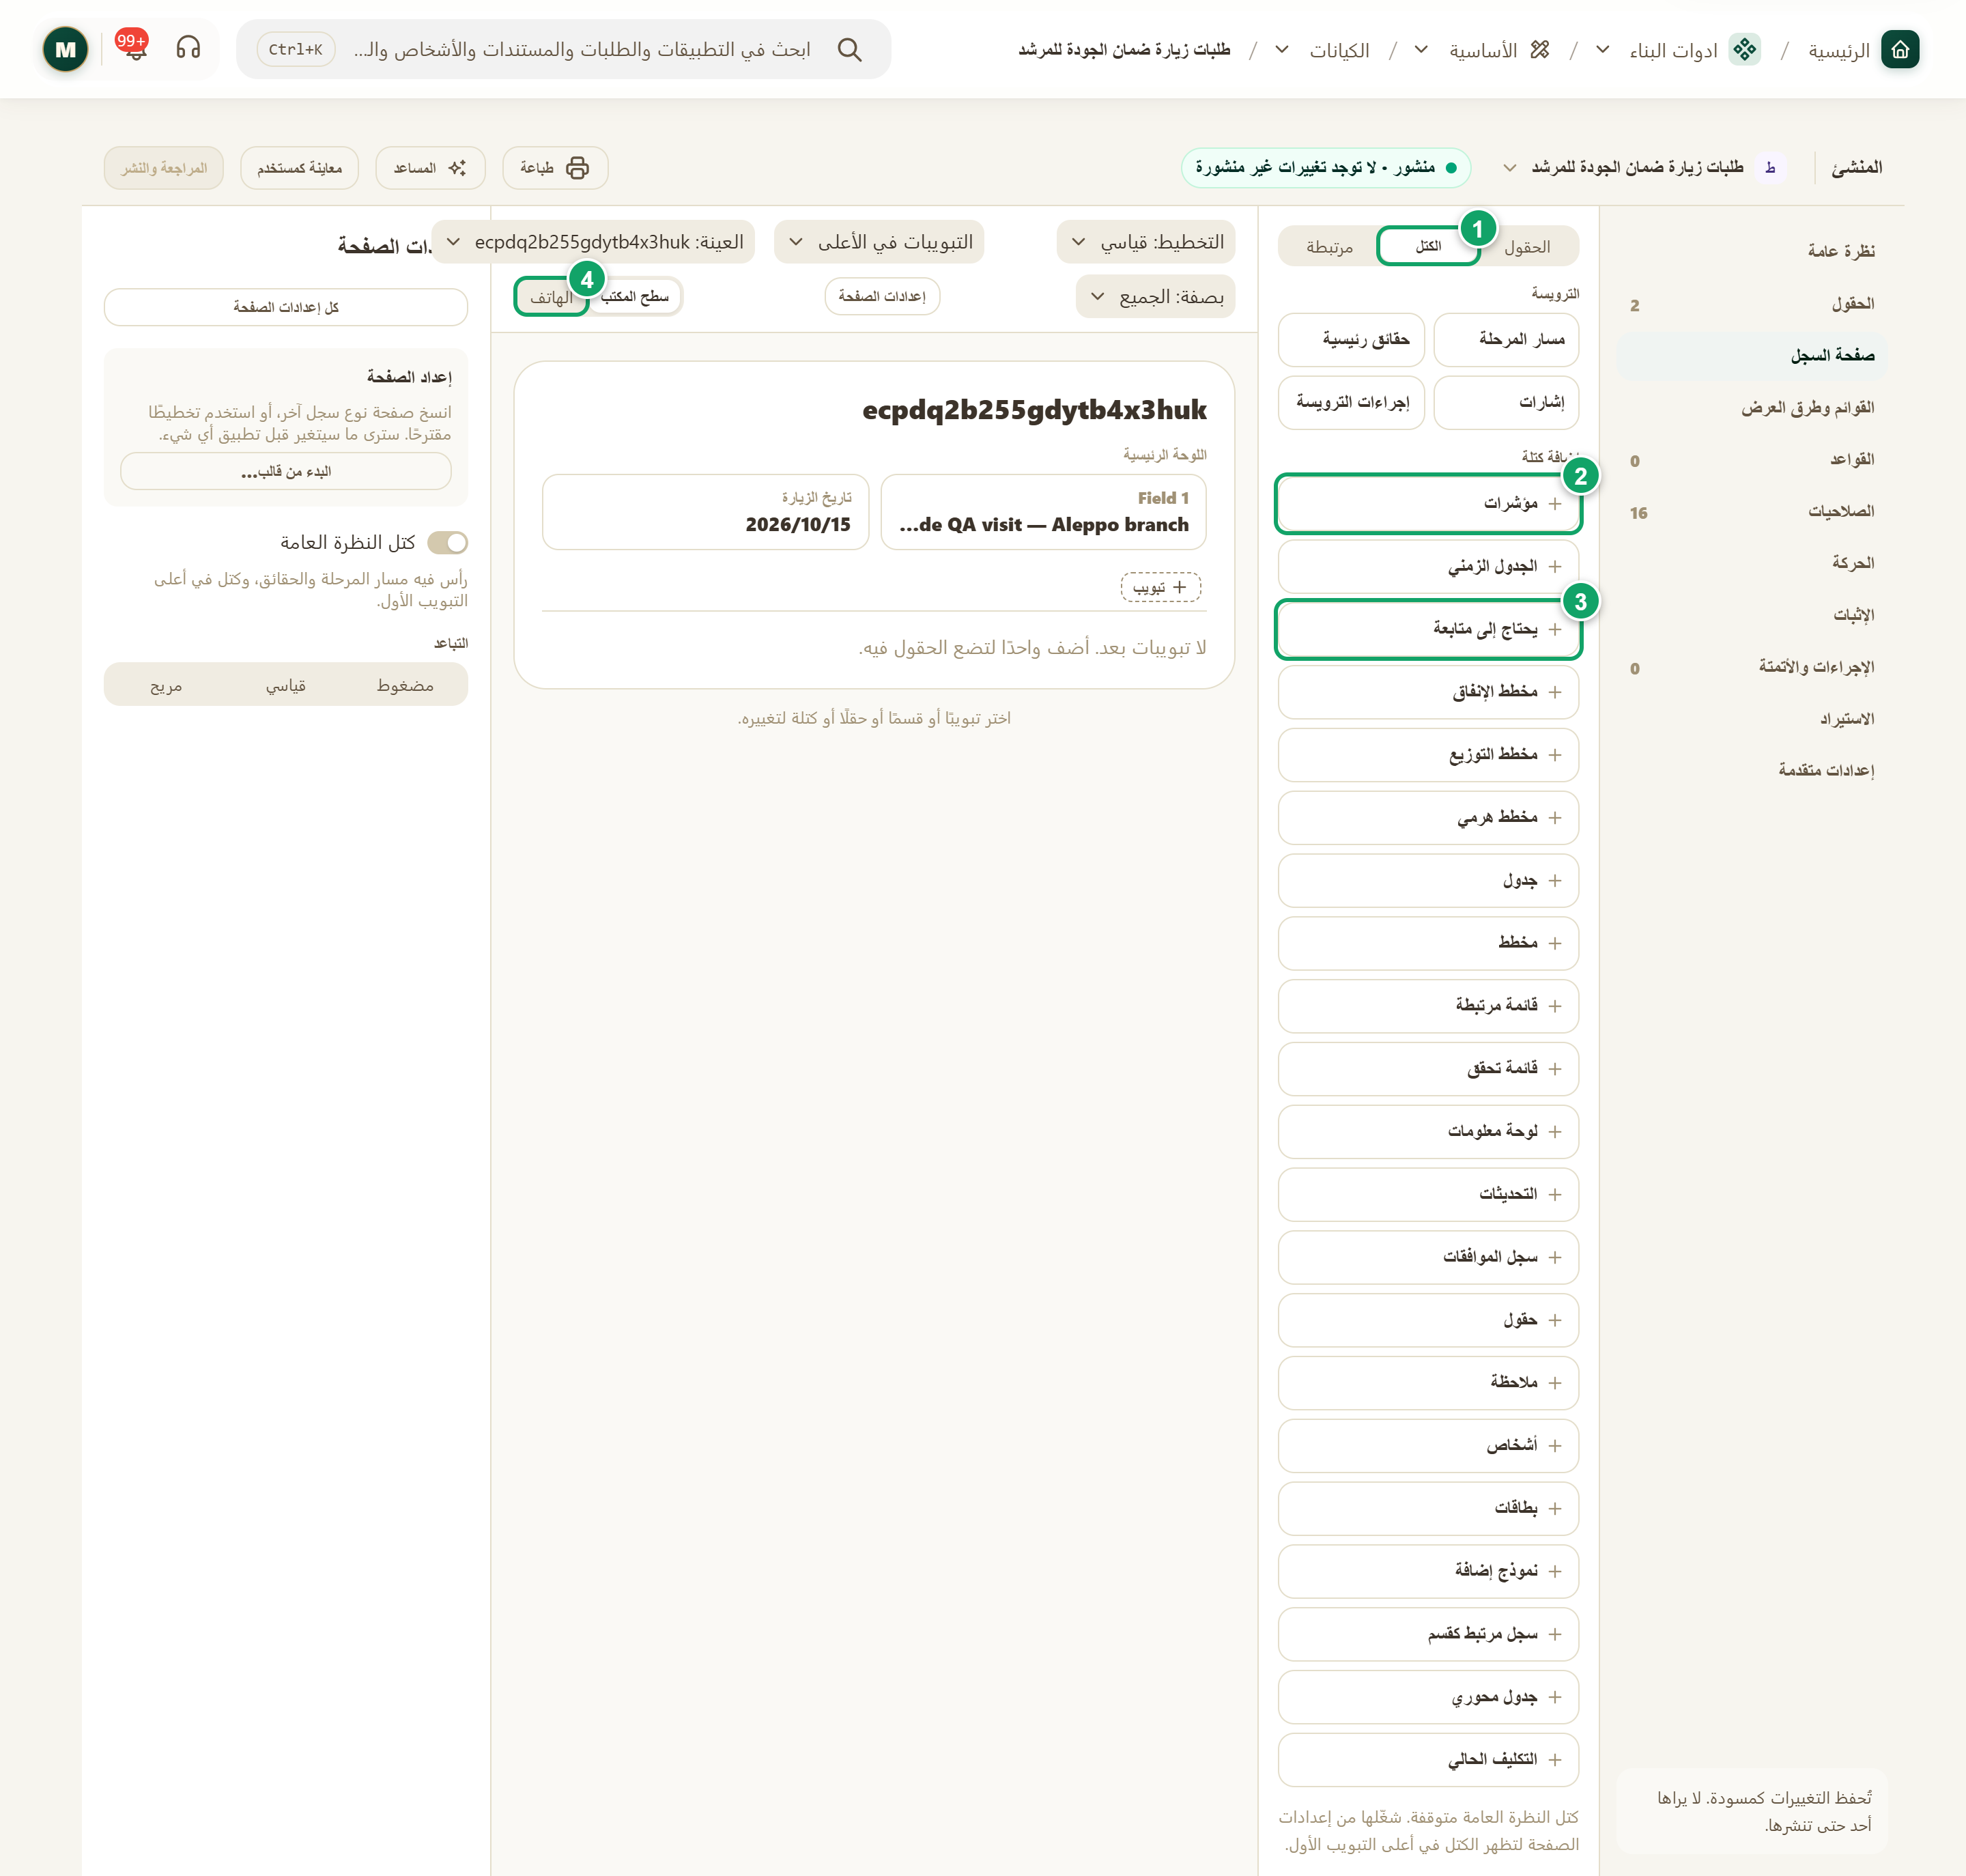
\includegraphics[width=0.95\linewidth,height=0.72\textheight,keepaspectratio]{figures/screens/ch06-ws-blocks-ar.png}
\caption{تبويب «الكتل» في «أجزاء الصفحة»}
\label{fig:builder-record-page-blocks-screen}
\shotnote{تعرض الصورة قسم «صفحة السجل» بعد فتح تبويب الكتل، وفيه كل الكتل التي يمكن وضعها أعلى التبويب الأول، والمعاينة إلى جانبها. ويفيدك ذلك في اختيار الكتلة ورؤية أثرها قبل النشر. ① «الكتل». ② «مؤشرات»: أرقام رئيسية عن السجل. ③ «يحتاج إلى متابعة»: تنبيهات بقواعد تحددها. ④ «الهاتف»: يعرض المعاينة بحجم شاشة الهاتف.}
\end{figure}

\begin{table}[H]
\centering
\caption{أجزاء الصفحة}
\label{tab:builder-record-page-blocks-parts}
\begin{tabularx}{\linewidth}{R{3.6cm} Y}
\rcHeaderRow
\thh{التبويب} & \thh{ما تضيفه منه}\\
الحقول & تسحب الحقل إلى مكانه في الصفحة. وتظهر الحقول غير الموضوعة في «ليست في الصفحة بعد»، والحقل يوجد في مكان واحد، فسحبه مرة أخرى ينقله.\\
الكتل & تختار كتلة لتضبطها، ثم تضيفها أعلى التبويب الأول.\\
مرتبطة & قوائم بالسجلات المرتبطة، وتوضع من حقل العلاقة في النوع المرتبط.\\
\end{tabularx}
\end{table}

\begin{table}[H]
\centering
\caption{أكثر الكتل استخداماً}
\label{tab:builder-record-page-blocks-kinds}
\begin{tabularx}{\linewidth}{R{3.6cm} Y}
\rcHeaderRow
\thh{الكتلة} & \thh{ما تعرضه}\\
مؤشرات & أرقاماً رئيسية، مثل نسبة الإنجاز، أو المستخدم من إجمالي، أو تأخر موعد.\\
يحتاج إلى متابعة & تنبيهات بقواعد تحددها، بدرجة «حرج» أو «تحذير» أو «معلومة»، مع عدد السجلات المطابقة أو قائمتها.\\
الجدول الزمني & المواعيد والمراحل من السجل والسجلات المرتبطة به على خط زمني.\\
قائمة مرتبطة وبطاقات & السجلات المرتبطة في جدول أو بطاقات داخل الصفحة.\\
سجل الموافقات والتحديثات & تاريخ الموافقات وآخر التحديثات على السجل.\\
ملاحظة وحقول وأشخاص & نصاً ثابتاً، أو مجموعة حقول، أو الأشخاص المرتبطين بالسجل.\\
مخطط ولوحة معلومات & رسماً بيانياً من بيانات السجل، أو لوحة معلومات جاهزة.\\
\end{tabularx}
\end{table}

\subsection{المعاينة والتخطيطات}

تعرض المعاينة الصفحة بسجل نموذجي من «العينة»، وتستطيع أن تراها «بصفة» دور معين، وبحجم «سطح المكتب» أو «الهاتف». أما «إدارة التخطيطات…» فتفتح نافذة «التخطيطات»: التخطيط يحفظ أنماط الأقسام وأعمدتها والمسافات والرأس وكتل النظرة العامة، أما التبويبات والأقسام ومواضع الحقول فمشتركة بين كل التخطيطات. وتحدد فيها التخطيط الافتراضي، أو تختار التخطيط من قيمة حقل في السجل.

\begin{figure}[H]
\centering
\begin{tikzpicture}[node distance=0.5cm]
\node[stepBox] (a) {\RL{تفعيل كتل النظرة العامة}};
\node[stepBox,below=of a] (b) {\RL{إضافة كتلة}};
\node[stepBox,below=of b] (c) {\RL{ضبط الكتلة وعرضها}};
\node[stepBox,below=of c] (d) {\RL{المعاينة بصفة دور}};
\node[stepBox,below=of d] (e) {\RL{المراجعة والنشر}};
\draw[flowsTo] (a) -- (b);
\draw[flowsTo] (b) -- (c);
\draw[flowsTo] (c) -- (d);
\draw[flowsTo] (d) -- (e);
\end{tikzpicture}
\rclegend
\caption{إضافة كتلة إلى صفحة السجل}
\label{fig:builder-record-page-blocks-flow}
\shotnote{يبدأ المخطط بتفعيل كتل النظرة العامة لأن تبويب «الكتل» لا يضيف شيئاً قبل ذلك. ثم تأتي المعاينة بصفة دور قبل النشر، لأن الكتلة قد تعرض أرقاماً من سجلات لا يحق لبعض الأدوار رؤيتها، فتتأكد مما يراه كل منهم.}
\end{figure}

\subsection{خطوات العمل والتحقق}
\begin{enumerate}
\item افتح «صفحة السجل»، ثم «إعدادات الصفحة»، وفعّل كتل النظرة العامة.
\item افتح «أجزاء الصفحة» ← «الكتل»، واختر الكتلة، ثم اضغط «إضافة كتلة».
\item اضبط الكتلة: العنوان والعرض («كامل العرض» أو «الثلثان» أو «الثلث») وما تعرضه، مثل قواعد «يحتاج إلى متابعة».
\item غيّر «بصفة» إلى دور آخر، و«حجم المعاينة» إلى «الهاتف»، وتأكد أن الصفحة واضحة في الحالتين، ثم انشر.
\end{enumerate}

\textbf{تحقق ومعالجة المشكلة:} يجب أن تظهر الكتلة أعلى التبويب الأول عند فتح سجل منشور. فإذا ظهر «كتل النظرة العامة متوقفة»، فاضغط «تشغيل كتل النظرة العامة» أولاً. وإذا كانت الكتلة فارغة، فجرّبها على سجل فيه البيانات التي تعتمد عليها.

\clearpage
\section{القوائم وطرق العرض}
\label{sec:builder-feature-lists}

يحدد قسم «القوائم وطرق العرض» كيف تظهر سجلات النوع معاً عندما يفتح المستخدم القائمة. فتختار طرق العرض التي يمكن التبديل بينها، مثل «جدول» أو «كانبان» أو «التقويم»، والأعمدة الظاهرة، والأرقام التي تلخّص القائمة في أعلاها. وتتيح بطاقة «الخلايا القابلة للتعديل» خيار «تعديل الخلايا في مكانها»، فيعدّل المستخدمون خلايا الجدول دون فتح كل سجل، بشرط أن تكون طرق عرض القوائم مفعّلة وأن يملكوا صلاحية تغيير الحقل.

\textbf{المسار ومن يستخدمه:} نوع السجلات ← «القوائم وطرق العرض». يستخدمه من يبني النوع، ويفيد كل من يتابع السجلات يومياً.

\begin{rcnote}[مثال: شركة الأفق]
يعرض مسؤول النظام طلبات الزيارة في «جدول» بأعمدة الرقم والفرع والموعد والحالة، ويضيف «التقويم» حسب موعد الزيارة، فترى سارة الخطيب زيارات الأسبوع في نظرة واحدة. ويبدأ بتفعيل المفتاح ① لاختيار الجدول والتقويم.
\end{rcnote}

\begin{figure}[H]
\centering
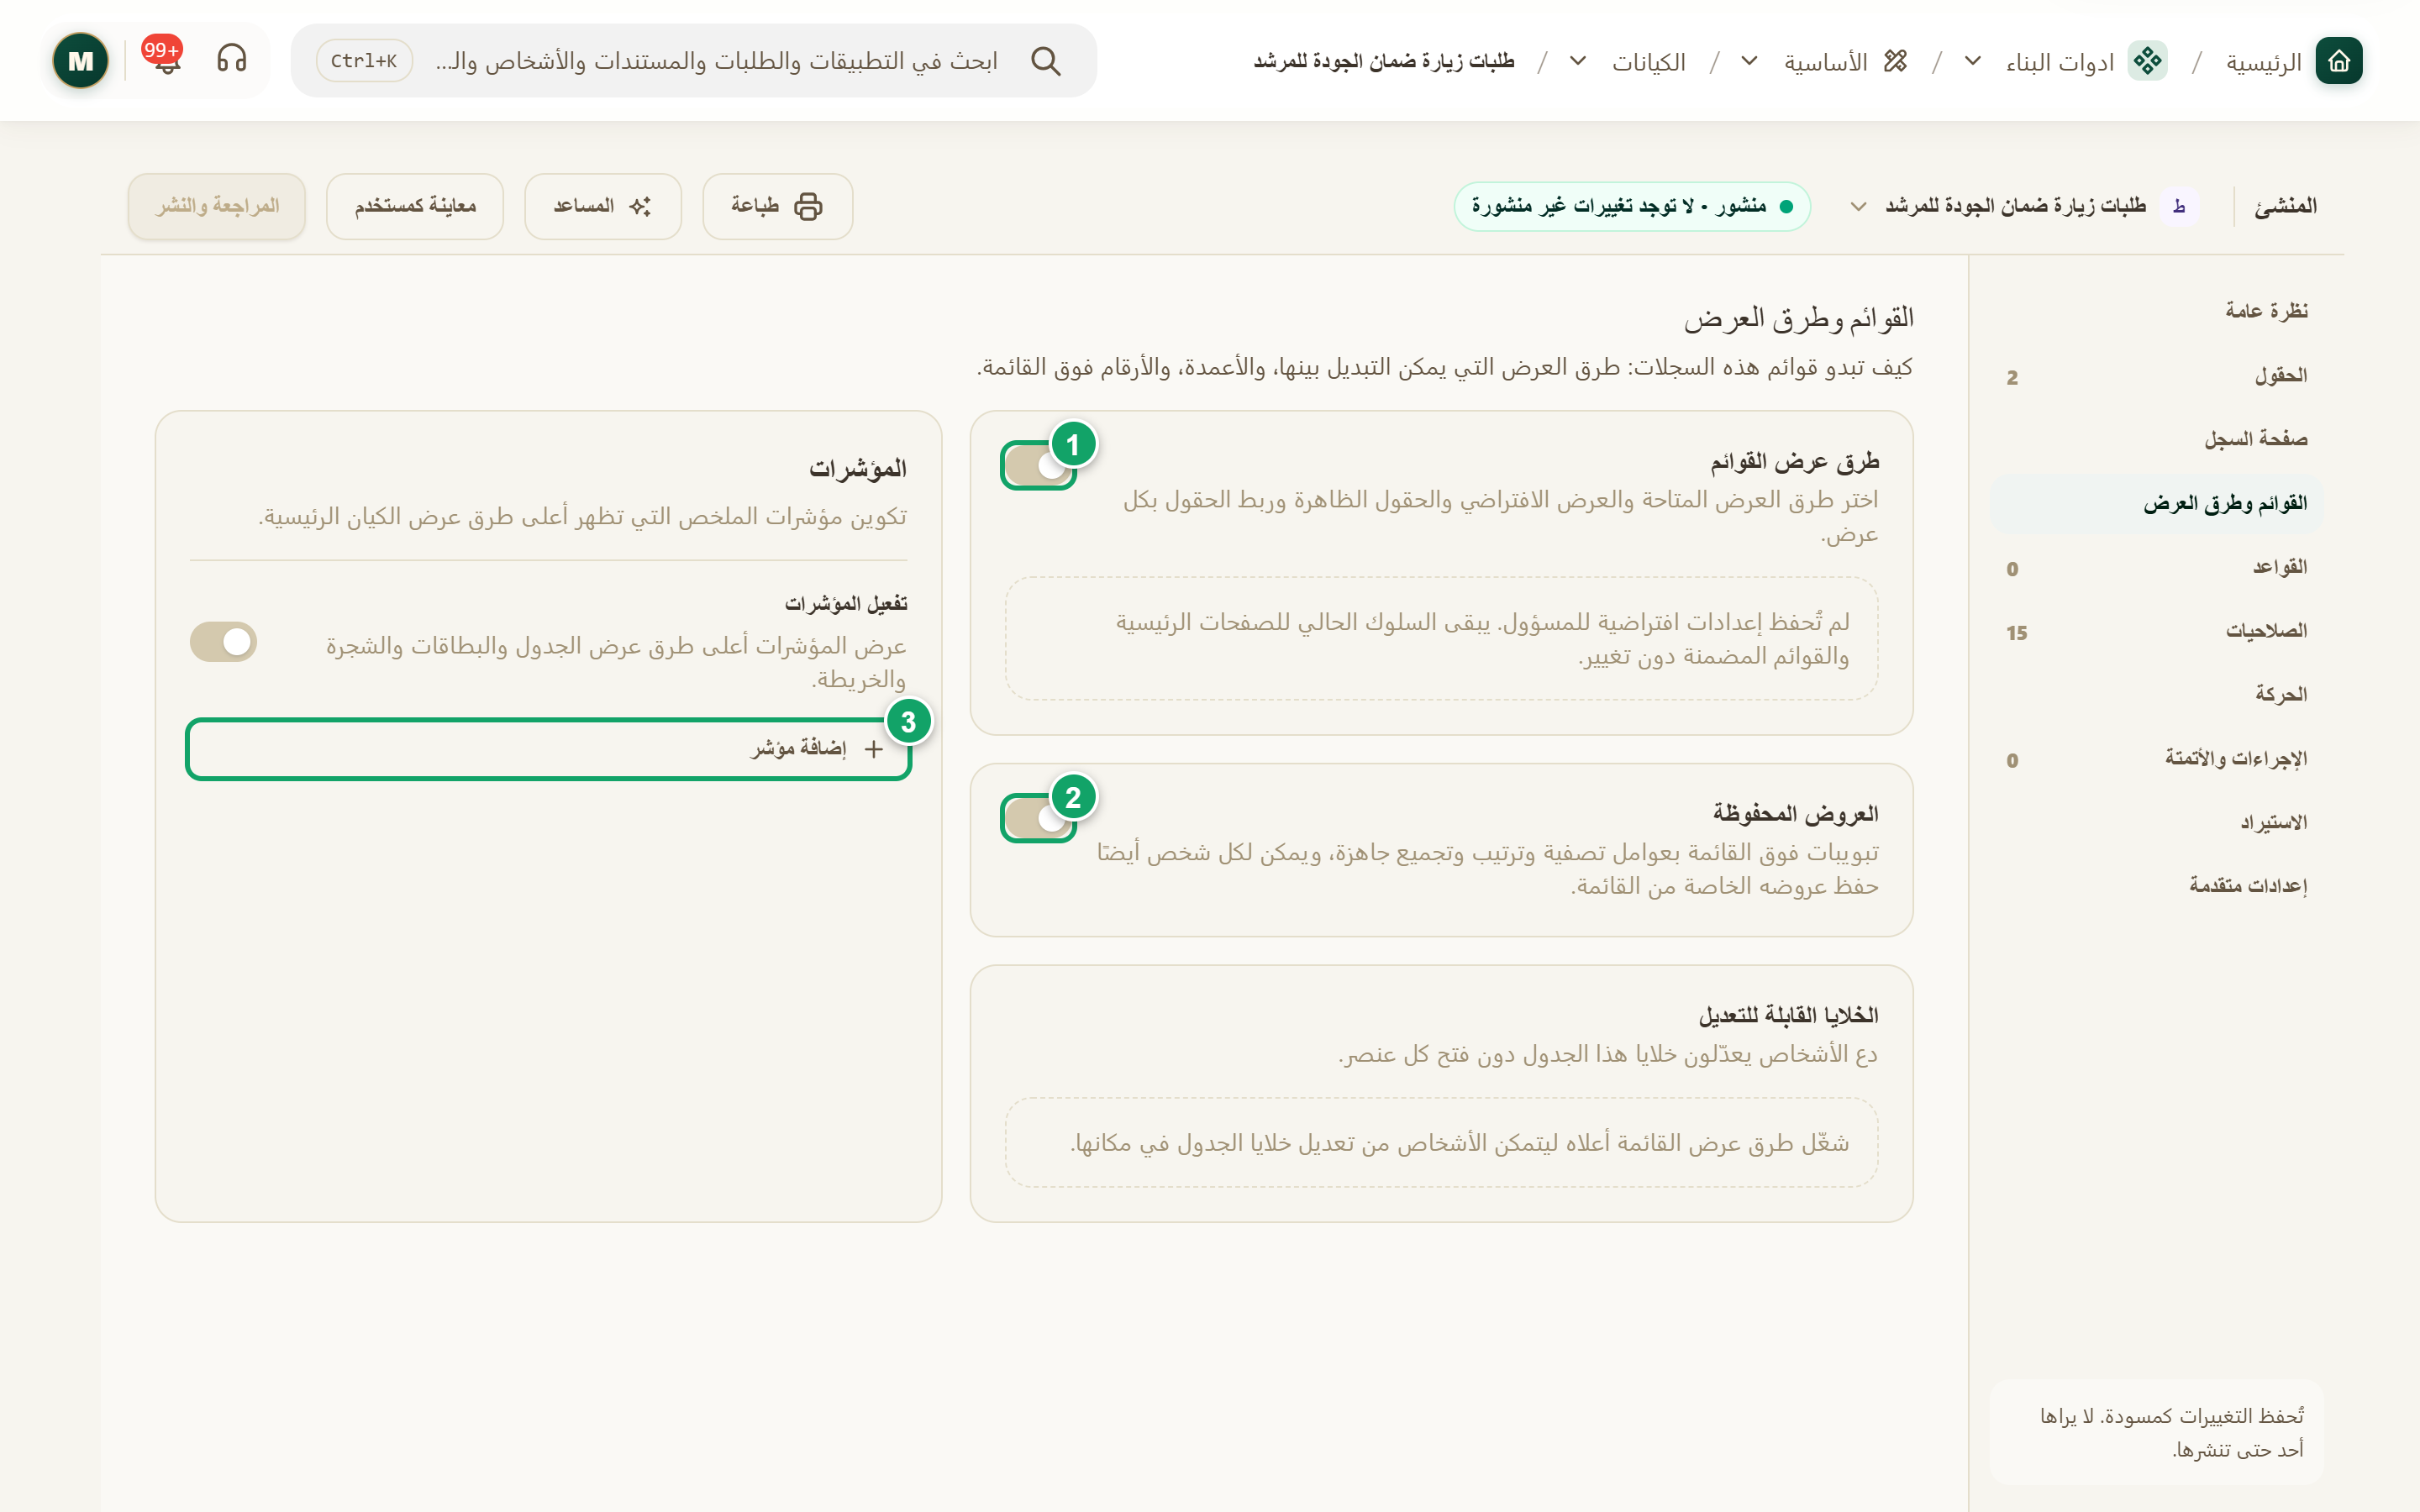
\includegraphics[width=0.95\linewidth,height=0.72\textheight,keepaspectratio]{figures/screens/ch06-ws-lists-ar.png}
\caption{قسم «القوائم وطرق العرض»}
\label{fig:builder-lists-screen}
\shotnote{يجمع القسم ما يتحكم في شكل قائمة السجلات. وكل المفاتيح متوقفة هنا، فتعمل القائمة بإعدادها الافتراضي. ① مفتاح «طرق عرض القوائم»: يتيح اختيار طرق العرض المتاحة والافتراضية والأعمدة. ② مفتاح «العروض المحفوظة»: يضيف تبويبات جاهزة فوق القائمة. ③ «إضافة مؤشر»: يضيف رقماً ملخصاً فوق القائمة.}
\end{figure}

\begin{figure}[H]
\centering
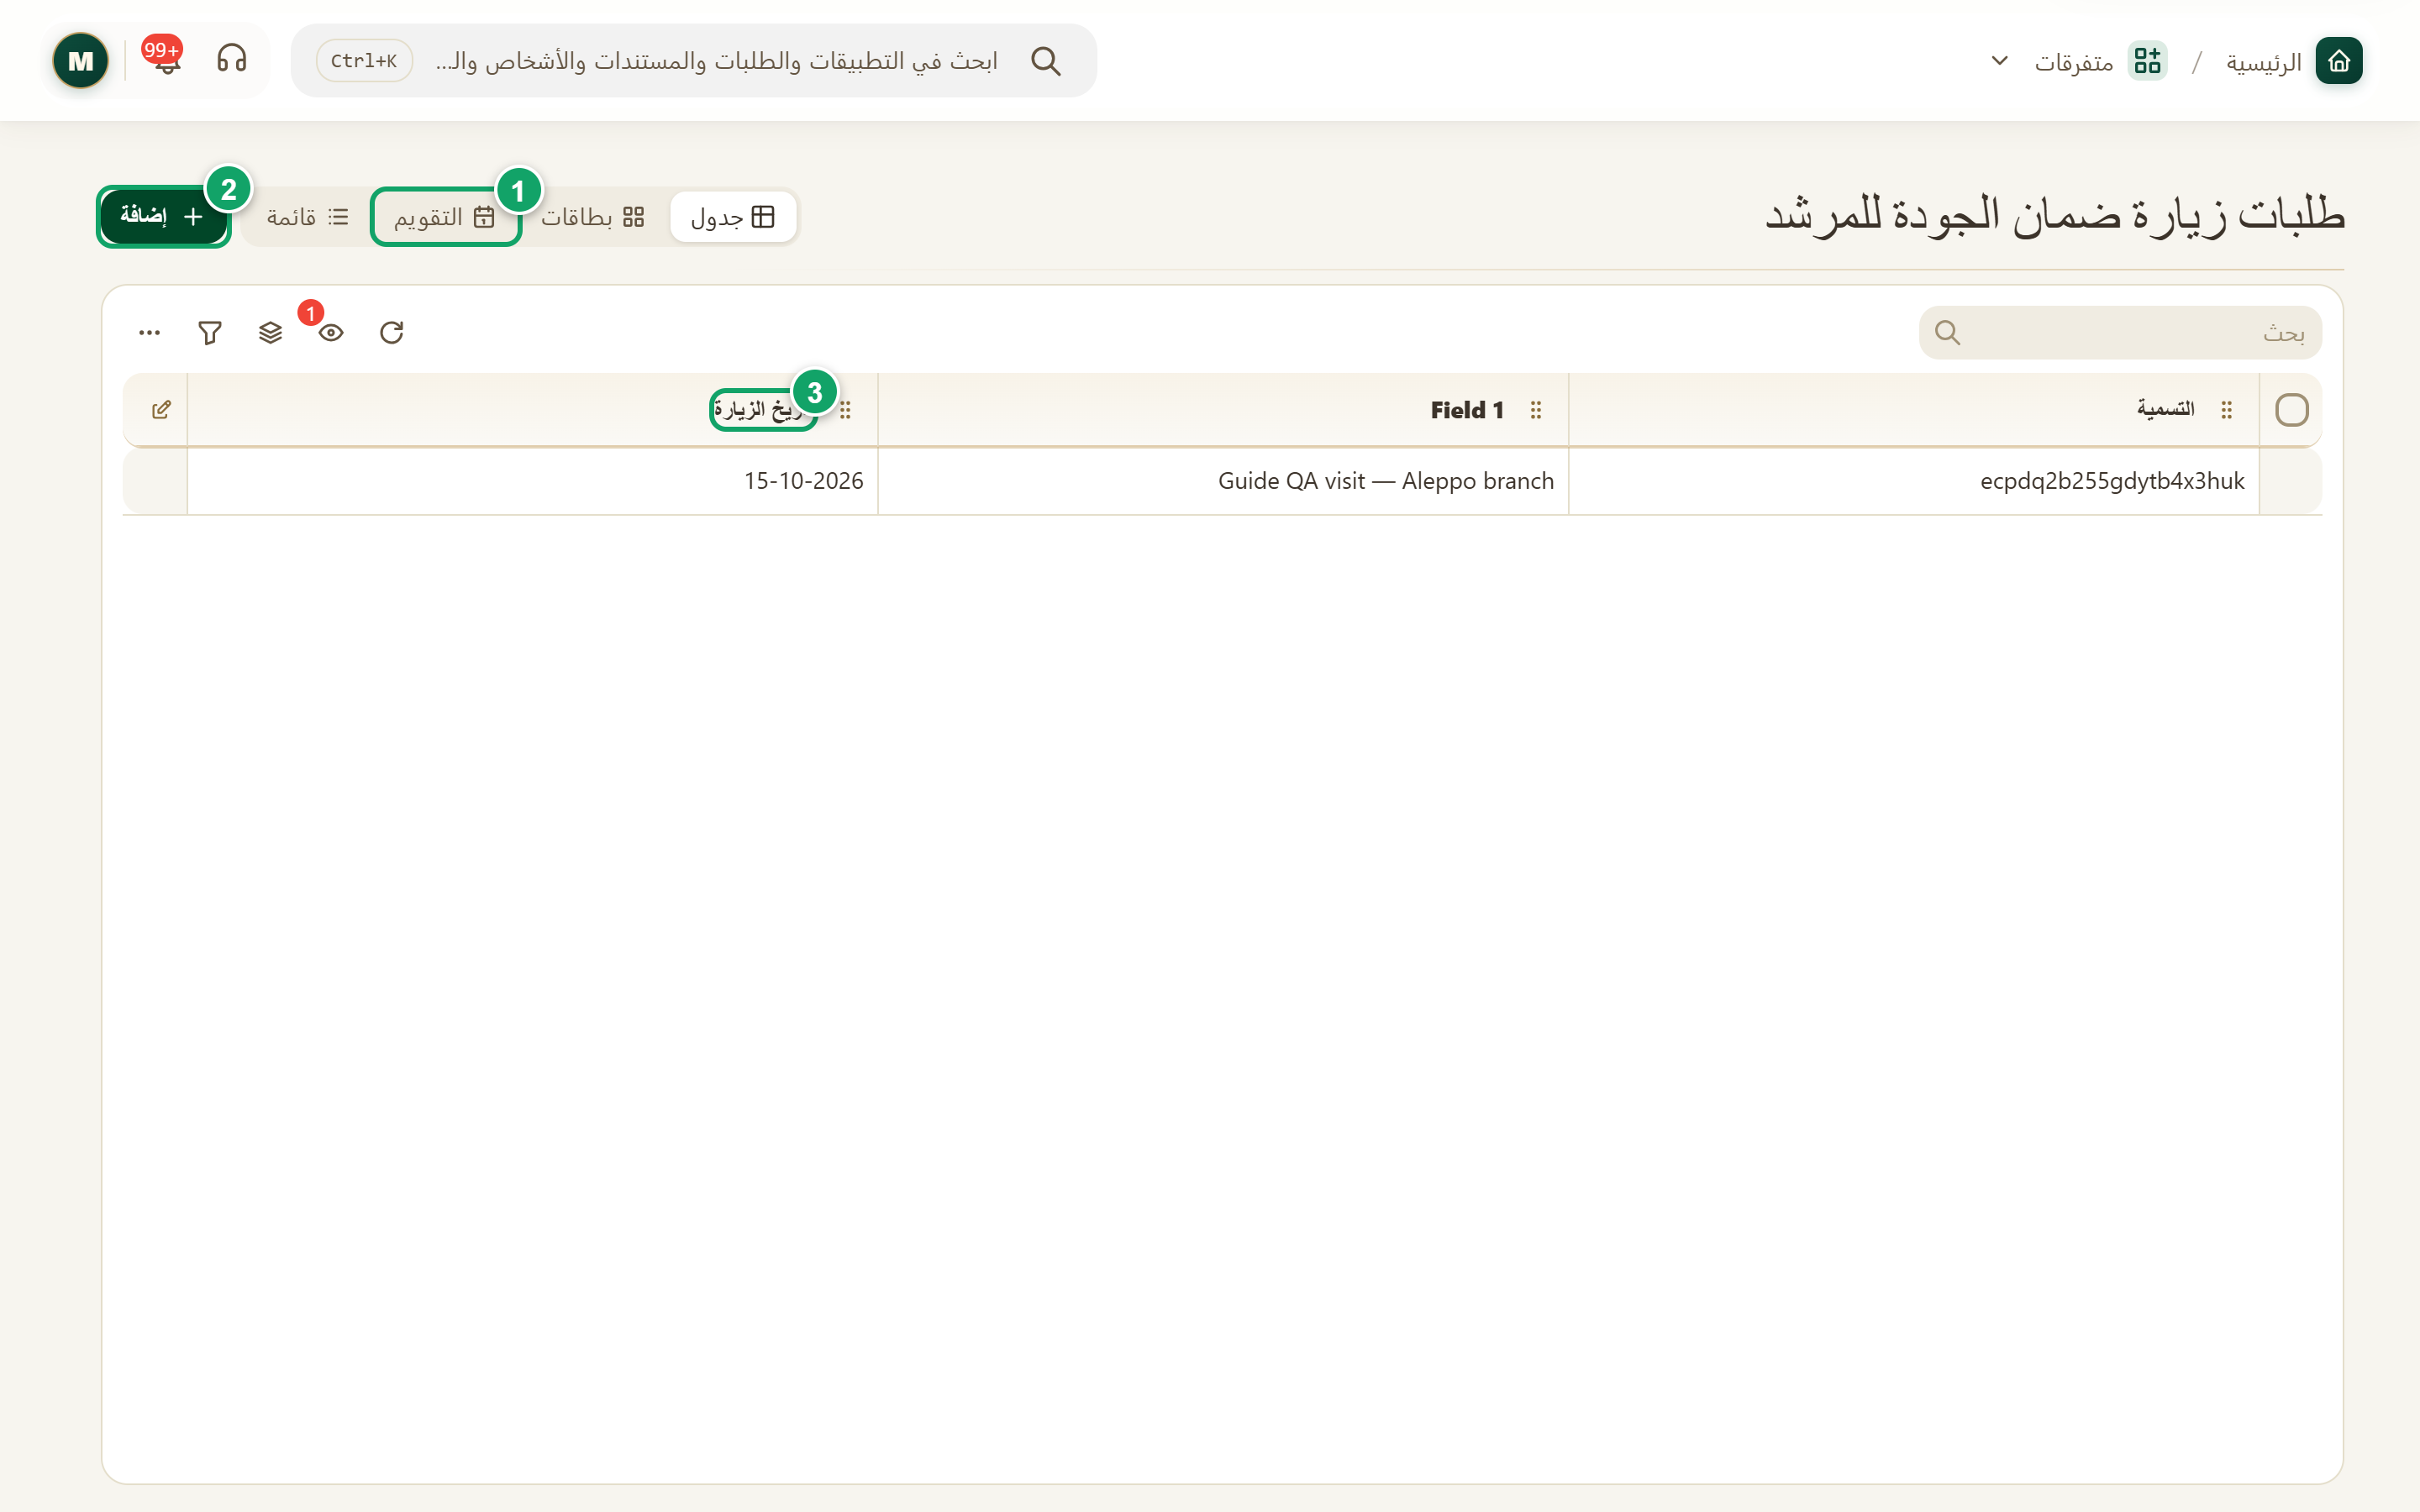
\includegraphics[width=0.95\linewidth,height=0.72\textheight,keepaspectratio]{figures/screens/ch06-records-ar.png}
\caption{قائمة سجلات النوع بعد النشر}
\label{fig:builder-lists-records}
\shotnote{هذه هي القائمة التي يراها المستخدمون بعد النشر، وفيها سجل اختبار أُنشئ في test2 ثم أُعيد فتحه للتحقق من الحفظ. ① «التقويم»: ظهرت طريقة العرض هذه لأن للنوع حقل تاريخ. ② «إضافة». ③ عمود «تاريخ الزيارة»: يعرض القيمة المحفوظة للسجل الاختباري بعد إعادة فتحه.}
\end{figure}


\begin{table}[H]
\centering
\caption{طرق العرض المتاحة}
\label{tab:builder-lists-modes}
\begin{tabularx}{\linewidth}{R{3.6cm} Y}
\rcHeaderRow
\thh{طريقة العرض} & \thh{متى تناسب}\\
جدول وقائمة & متاحان دائماً لمراجعة السجلات ومقارنتها صفاً صفاً، مع الترتيب والتصفية.\\
بطاقات ومعرض & «بطاقات» متاحة دائماً، أما «معرض» فيظهر عندما يكون للنوع حقل «ملف» تُعرض منه الصور.\\
كانبان & يوزّع السجلات في أعمدة حسب الحالة أو قيمة اختيار، ويظهر عندما يوجد حقل مناسب لذلك.\\
التقويم والخط الزمني & يظهران عندما يكون للنوع حقل تاريخ أو نطاق زمني، مثل المواعيد والمراحل.\\
خريطة & تظهر عندما يكون للنوع حقل «موقع» أو «حدود».\\
شجرة & تظهر عندما تفعّل «السجلات الأم» في «إعدادات متقدمة»، فتُعرض السجلات في تسلسل أب وأبناء.\\
\end{tabularx}
\end{table}

\begin{figure}[H]
\centering
\begin{tikzpicture}[node distance=0.5cm]
\node[entity] (fields) {\RL{الحقول}};
\node[entityOpt,below right=0.7cm and 0.3cm of fields] (cal) {\RL{التقويم}};
\node[entityOpt,below left=0.7cm and 0.3cm of fields] (map) {\RL{خريطة}};
\draw[dependsOnOpt] (fields.south) -- ++(0,-0.3) -| (cal.north);
\draw[dependsOnOpt] (fields.south) -- ++(0,-0.3) -| (map.north);
\end{tikzpicture}
\rclegend
\caption{طرق عرض تعتمد على نوع الحقل}
\label{fig:builder-lists-depends}
\shotnote{يوضّح الشكل أن بعض طرق العرض تحتاج إلى حقل من نوع معيّن: فالتقويم يحتاج إلى تاريخ، والخريطة تحتاج إلى موقع أو حدود. لذلك إذا لم تجد طريقة عرض تريدها، فراجع الحقول أولاً، لأن الطريقة لا تظهر في الخيارات دون الحقل الذي تعتمد عليه.}
\end{figure}

\subsection{خطوات العمل والتحقق}
\begin{enumerate}
\item افتح نوع السجلات واختر «القوائم وطرق العرض».
\item فعّل طرق العرض التي يحتاجها الفريق، واختر الطريقة الافتراضية التي تظهر أولاً.
\item اختر الأعمدة الظاهرة ورتّبها حسب أهميتها للعمل اليومي، وأضف الأرقام الملخّصة عند الحاجة.
\end{enumerate}

\textbf{تحقق ومعالجة المشكلة:} يجب أن تعرض «نظرة عامة» الطريقة الافتراضية وعدد العروض المحفوظة. وبعد النشر افتح قائمة السجلات وبدّل بين الطرق للتأكد منها؛ فإذا كانت طريقة العرض فارغة، فتحقق من أن السجلات تحمل قيمة في الحقل الذي تعتمد عليه.

\clearpage
\section{المؤشرات والعروض المحفوظة}
\label{sec:builder-feature-figures-views}

تساعد هاتان الأداتان الفريق على فهم القائمة دون أن يفتح كل سجل. فـ«المؤشرات» أرقام تلخيصية تظهر فوق القائمة، مثل عدد الطلبات المفتوحة أو مجموع المبالغ، والضغط على أي مؤشر يصفّي القائمة. أما «العروض المحفوظة» فتبويبات فوق القائمة، لكل منها تصفية وترتيب وتجميع جاهز، فينتقل المستخدم بين «طلباتي» و«بانتظار المراجعة» بضغطة واحدة.

\textbf{المسار ومن يستخدمه:} «المنشئ» ← «القوائم وطرق العرض» ← بطاقة «المؤشرات» وبطاقة «العروض المحفوظة». يضبطها من يبني النوع، ويراها كل من يفتح القائمة. ويستطيع كل مستخدم أن يحفظ عروضاً خاصة به من القائمة نفسها.

\begin{rcnote}[مثال: شركة الأفق]
يضيف المسؤول فوق قائمة «طلبات الزيارة» مؤشراً بعدد الطلبات «قيد المراجعة» يظهر بلون التحذير إذا زاد على خمسة، وعرضاً محفوظاً باسم «بانتظار مراجعتي» يعرض لسارة الخطيب الطلبات التي تنتظرها.
\end{rcnote}

\begin{figure}[H]
\centering
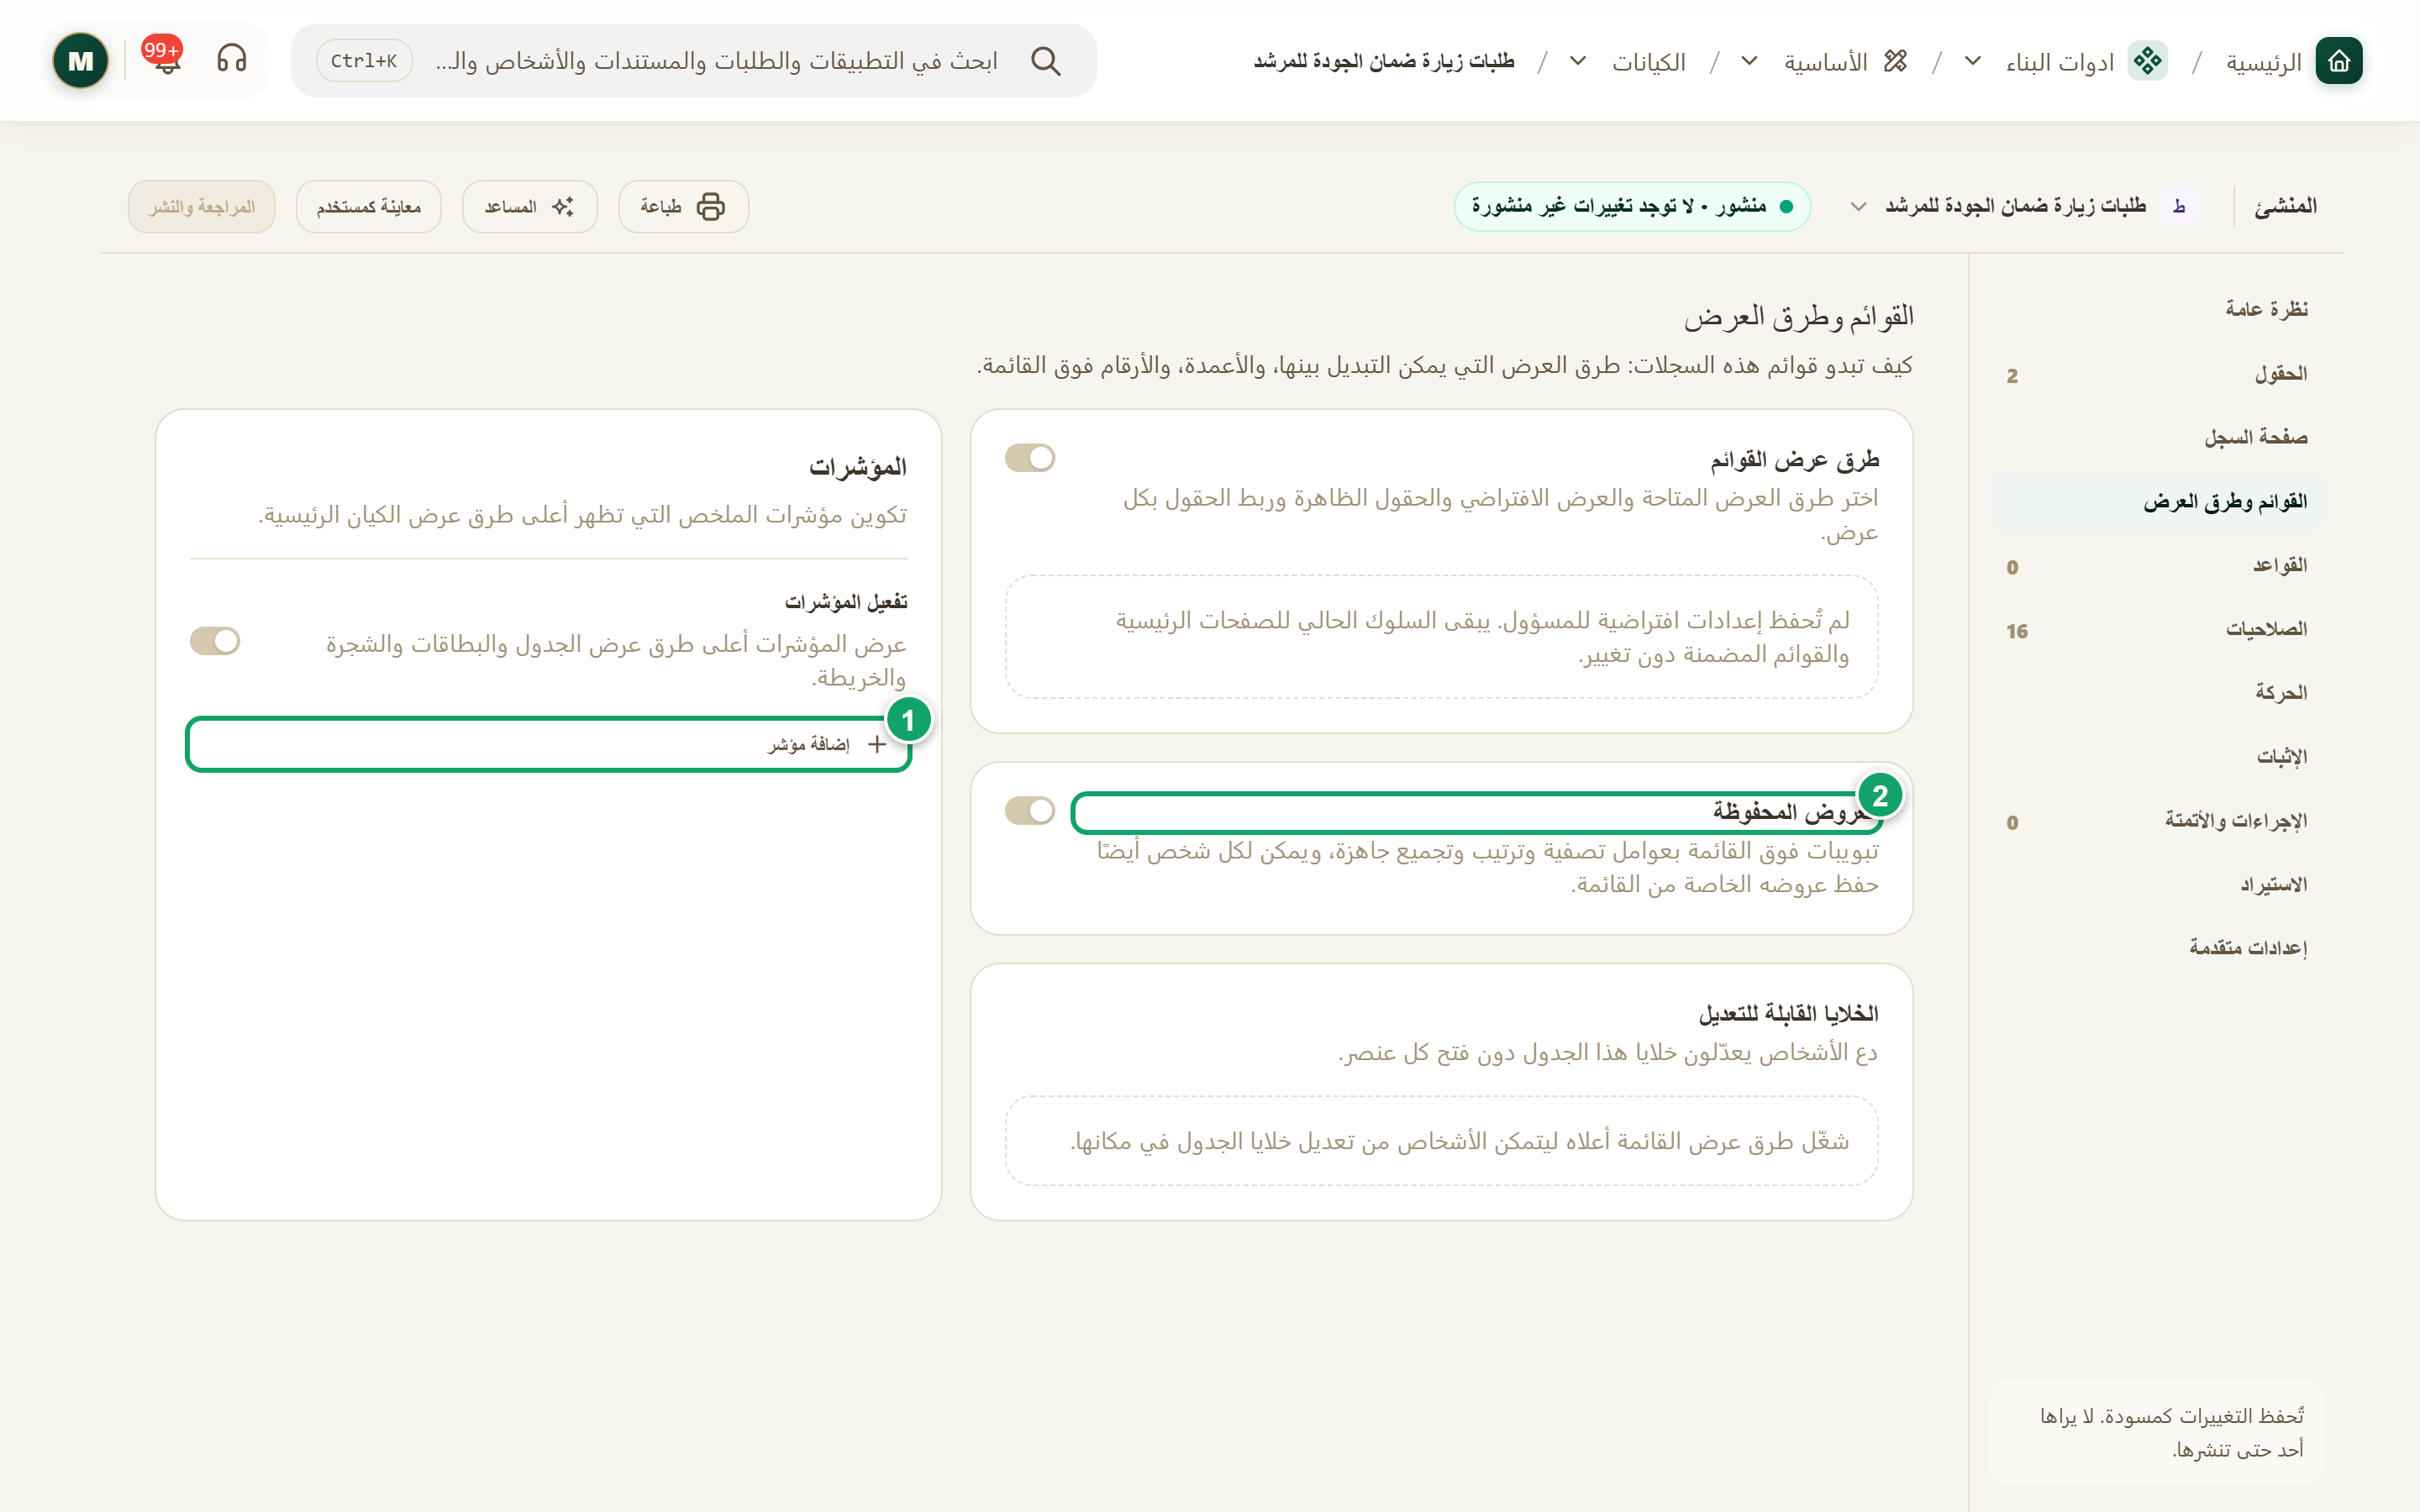
\includegraphics[width=0.95\linewidth,height=0.72\textheight,keepaspectratio]{figures/screens/ch06-ws-figures-views-ar.png}
\caption{بطاقتا المؤشرات والعروض المحفوظة في «القوائم وطرق العرض»}
\label{fig:builder-figures-views-screen}
\shotnote{تعرض الصورة قسم «القوائم وطرق العرض» في النوع الاختباري، ولم يُضف إليه بعد أي مؤشر أو عرض محفوظ. ويبيّن ذلك أين تبدأ عندما تريد تلخيص القائمة أو تنظيمها. ① «إضافة مؤشر»: يضيف رقماً تلخيصياً فوق القائمة. ② «العروض المحفوظة»: البطاقة التي تضيف منها تبويبات جاهزة فوق القائمة.}
\end{figure}

\begin{table}[H]
\centering
\caption{إعدادات المؤشر}
\label{tab:builder-figures-settings}
\begin{tabularx}{\linewidth}{R{3.6cm} Y}
\rcHeaderRow
\thh{الإعداد} & \thh{المعنى}\\
نوع المؤشر & «قيمة واحدة»، أو «نسبة (جزء من إجمالي)» تُعرض مع شريط، أو «التوزيع حسب الحالة».\\
الحساب & العدد، أو المجموع، أو المتوسط، أو الأدنى، أو الأعلى، أو المتوسط المرجّح لحقل رقمي.\\
السجلات المحسوبة & سجلات هذا النوع أو نوع مرتبط به، مع فلاتر ونطاق تاريخ، مثل آخر ثلاثين يوماً.\\
سطر تحت المؤشر & لا شيء، أو نص، أو قيمة ثانية، أو أقرب سجل قادم.\\
التمييز & يلوّن المؤشر بلون «تحذير» أو «حرج» عندما تقل القيمة عن حد أو تزيد عليه.\\
\end{tabularx}
\end{table}

\begin{table}[H]
\centering
\caption{ما يحفظه العرض المحفوظ}
\label{tab:builder-saved-views-settings}
\begin{tabularx}{\linewidth}{R{3.6cm} Y}
\rcHeaderRow
\thh{الإعداد} & \thh{المعنى}\\
الاسم واللون & اسم التبويب ولونه فوق القائمة، ويمكن أن يظهر عليه عدد السجلات.\\
يفتح في & طريقة العرض التي يفتح بها التبويب، أو الإبقاء على طريقة العرض الحالية.\\
الترتيب والتجميع & الحقل الذي تُرتب به السجلات واتجاه الترتيب، والحقل الذي تُجمع حسبه.\\
الفلاتر & الشروط التي تحدد السجلات الظاهرة، ويمكن أن تتبع المستخدم نفسه، مثل «أنا» أو عدد أيام من اليوم.\\
السجلات التي يستطيع المستخدم العمل عليها & يعرض فقط السجلات التي يستطيع المستخدم تنفيذ انتقال عليها في حقل الحالة.\\
\end{tabularx}
\end{table}

\begin{figure}[H]
\centering
\begin{tikzpicture}[node distance=0.5cm]
\node[stepBox] (a) {\RL{تفعيل المؤشرات}};
\node[stepBox,below=of a] (b) {\RL{إضافة مؤشر وضبطه}};
\node[stepBox,below=of b] (c) {\RL{إضافة عرض محفوظ}};
\node[stepBox,below=of c] (d) {\RL{المراجعة والنشر}};
\node[stepBox,below=of d] (e) {\RL{التجربة في القائمة}};
\draw[flowsTo] (a) -- (b);
\draw[flowsTo] (b) -- (c);
\draw[flowsTo] (c) -- (d);
\draw[flowsTo] (d) -- (e);
\end{tikzpicture}
\rclegend
\caption{تلخيص القائمة وتنظيمها}
\label{fig:builder-figures-views-flow}
\shotnote{يجمع المخطط الأداتين في مسار واحد لأنهما تعملان فوق القائمة نفسها: المؤشر يلخّص والعرض المحفوظ يصفّي. وينتهي بالتجربة في القائمة بعد النشر، لأن الضغط على المؤشر والتنقل بين التبويبات لا يظهران إلا هناك.}
\end{figure}

\subsection{خطوات العمل والتحقق}
\begin{enumerate}
\item افتح «القوائم وطرق العرض»، وفعّل «تفعيل المؤشرات»، ثم اضغط «إضافة مؤشر».
\item اختر نوع المؤشر والحساب والحقل، وأضف الفلاتر ونطاق التاريخ، ثم حدد التمييز إن احتجت إلى تنبيه بصري.
\item في «العروض المحفوظة» فعّل إظهار التبويبات، واضغط «إضافة عرض»، واكتب اسمه وفلاتره وترتيبه.
\item انشر التغييرات، ثم افتح القائمة واضغط المؤشر والتبويب الجديد.
\end{enumerate}

\textbf{تحقق ومعالجة المشكلة:} يجب أن يظهر المؤشر فوق القائمة، وأن يصفّيها عند الضغط عليه، وأن يعرض التبويب السجلات المطابقة لفلاتره. فإذا لم يظهر المؤشر، فتأكد أن «تفعيل المؤشرات» مفعّل وأن المؤشر غير مخفي. وتذكّر أن العروض التي تضيفها هنا يراها الجميع، أما «حفظ العرض» في القائمة فيحفظ عرضاً لا يراه غيرك.

\clearpage
\section{القواعد}
\label{sec:builder-feature-rules}

القاعدة تجعل السجل يتصرف بحسب ما فيه من قيم، دون أن يتذكر المستخدم ذلك بنفسه. فقد تُظهر حقلاً عند اختيار قيمة معينة، أو تقفله بعد الإنشاء، أو تجعله إلزامياً في حالة محددة، أو ترفض قيمة غير منطقية. ويجمع قسم «القواعد» هذه القواعد كلها في قائمة واحدة.

\textbf{المسار ومن يستخدمه:} نوع السجلات ← «القواعد». يستخدمه من يبني النوع، بعد أن تكتمل الحقول.

\begin{rcnote}[مثال: شركة الأفق]
يضيف مسؤول النظام قاعدة تُظهر حقل «سبب الرفض» عندما تكون الحالة «مرفوض» فقط، وقاعدة تتحقق من أن موعد الزيارة يقع في تاريخ الطلب أو بعده. ويضيف القاعدتين من ①.
\end{rcnote}

\begin{figure}[H]
\centering
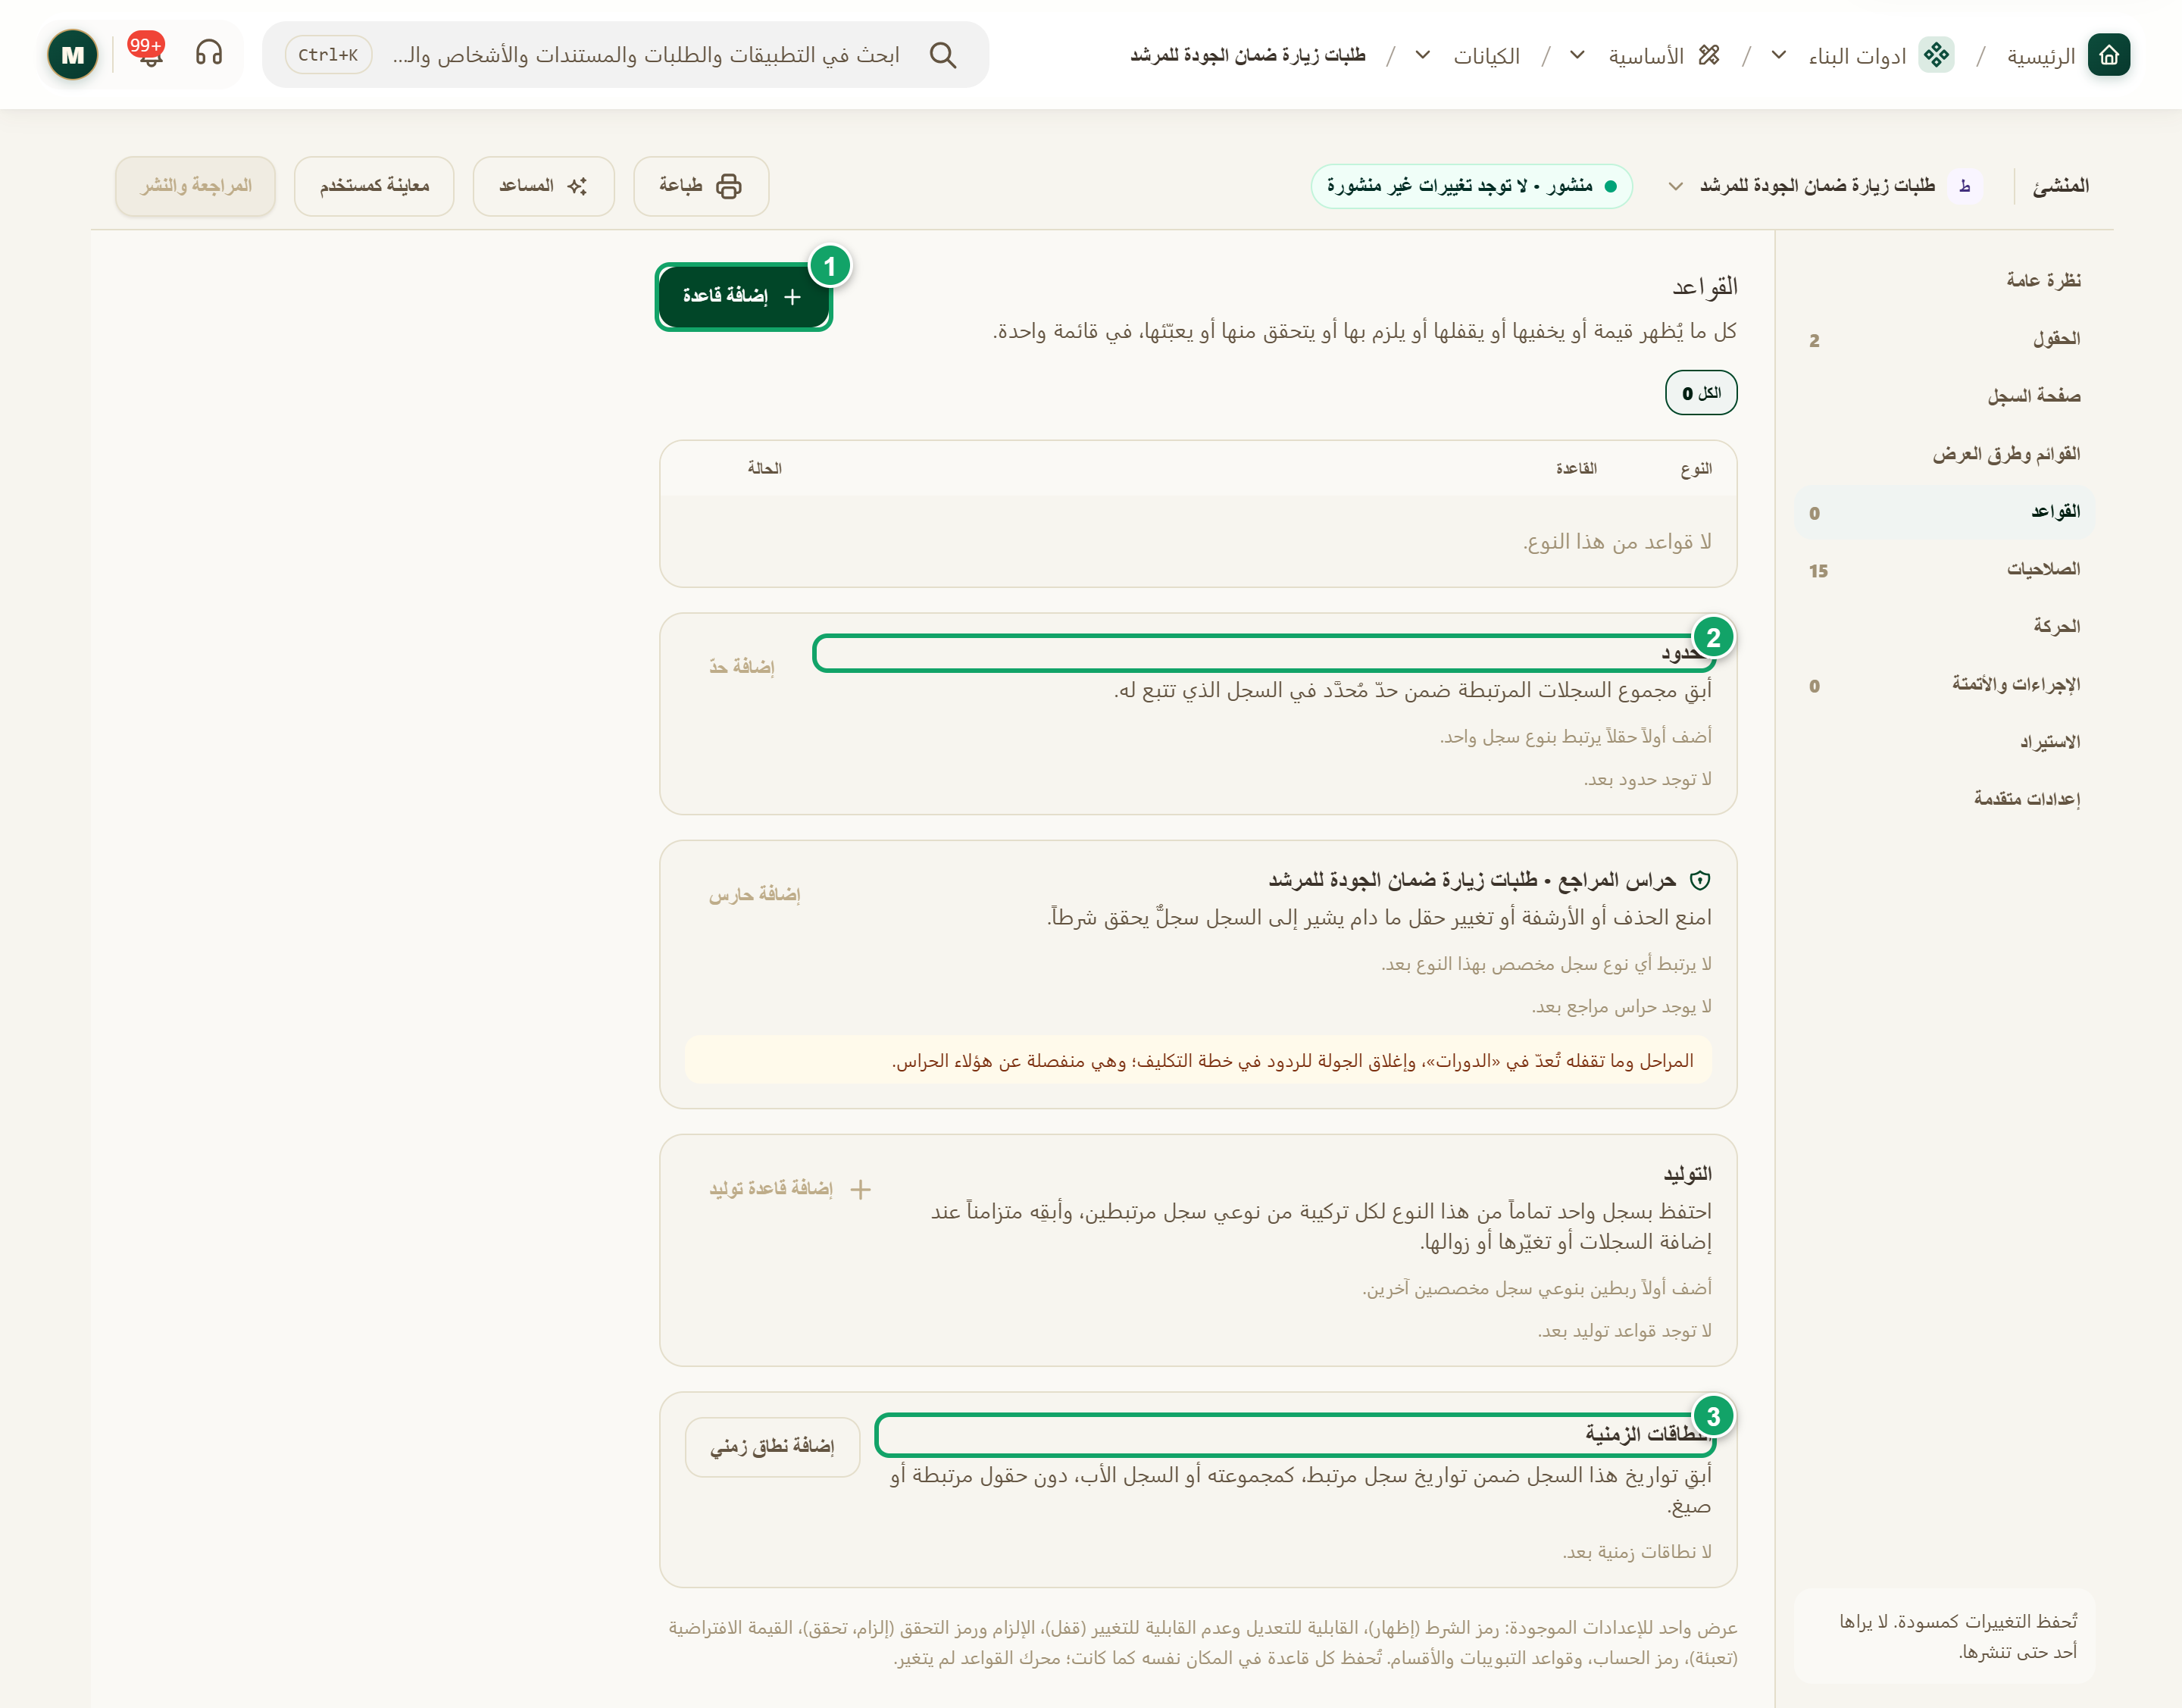
\includegraphics[width=0.95\linewidth,height=0.72\textheight,keepaspectratio]{figures/screens/ch06-ws-rules-ar.png}
\caption{قسم «القواعد» وأدواته الإضافية}
\label{fig:builder-rules-screen}
\shotnote{تظهر في أعلى القسم قائمة القواعد، وتحتها أدوات أخرى تحمي البيانات، مثل الحدود والنطاقات الزمنية. والقائمة فارغة لأن النوع الاختباري بلا قواعد. ① «إضافة قاعدة». ② «الحدود»: تُبقي مجموع السجلات المرتبطة ضمن حدّ. ③ «النطاقات الزمنية»: تُبقي تواريخ السجل ضمن تواريخ سجل مرتبط.}
\end{figure}


\begin{table}[H]
\centering
\caption{أنواع القواعد}
\label{tab:builder-rules-kinds}
\begin{tabularx}{\linewidth}{R{3.6cm} Y}
\rcHeaderRow
\thh{النوع} & \thh{ماذا تفعل؟}\\
إظهار أو إخفاء & تُظهر حقلاً أو تبويباً أو قسماً عندما يتحقق شرط، وتخفيه في غير ذلك.\\
قفل التعديل & تمنع تغيير حقل أو تبويب أو قسم: «مقفل عندما» يتحقق شرط، أو «قابل للتعديل فقط عندما»، أو «بعد الإنشاء».\\
إلزام & تجعل الحقل إلزامياً «دائمًا» أو «فقط عندما» يتحقق شرط، مع رسالة توضح السبب.\\
تحقق من القيمة & ترفض القيمة إن لم تكن، مثلاً، أكبر من رقم أو بعد تاريخ أو مختلفة عن حقل آخر، وتعرض رسالتك.\\
تعبئة قيمة & تبدأ الحقل بقيمة جاهزة يستطيع المستخدم تغييرها.\\
حساب & تعرض الحقول المحسوبة؛ وتعديلها يتم من قسم «الحقول».\\
\end{tabularx}
\end{table}

\begin{table}[H]
\centering
\caption{قواعد أخرى ليست في هذا القسم}
\label{tab:builder-rules-other}
\begin{tabularx}{\linewidth}{R{3.6cm} Y}
\rcHeaderRow
\thh{القاعدة} & \thh{أين تجدها؟}\\
الحدود & أسفل قائمة القواعد: تُبقي مجموع السجلات المرتبطة أو عددها ضمن حدّ، ثم ترفض التجاوز أو تنبّه وتطلب تبريراً.\\
قواعد دورة الحياة & في حقل «الحالة» داخل «الحقول»: لكل حالة تحدد إن كان السجل «مقفل» أو «مقفل باستثناء…»، ويمكنك «منع الحذف». تحتاج إلى قالب حالات ثابت.\\
القيم الفريدة & في «إعدادات متقدمة»: تمنع تكرار رمز أو مجموعة قيم بين سجلين.\\
\end{tabularx}
\end{table}

\begin{figure}[H]
\centering
\begin{tikzpicture}[node distance=0.5cm]
\node[stepBox] (a) {\RL{اختيار نوع القاعدة}};
\node[stepBox,below=of a] (b) {\RL{الشرط: عندما…}};
\node[stepBox,below=of b] (c) {\RL{الهدف: حقل أو تبويب أو قسم}};
\node[stepBox,below=of c] (d) {\RL{جرّبها ثم احفظ في المسودة}};
\draw[flowsTo] (a) -- (b);
\draw[flowsTo] (b) -- (c);
\draw[flowsTo] (c) -- (d);
\end{tikzpicture}
\rclegend
\caption{كيف تُبنى القاعدة}
\label{fig:builder-rules-flow}
\shotnote{تُقرأ القاعدة كجملة: «عندما» يتحقق شرط، نفّذ أثراً على هدف محدد. ويضع المخطط التجربة قبل الحفظ، لأن «جرّبها» يطبّق القاعدة على سجلات عينة فيكشف الشرط الخاطئ قبل أن يصل إلى المستخدمين. وتنطبق القواعد على كل من يستطيع تعديل السجل، فلا تُستخدم لتمييز دور من آخر.}
\end{figure}

\subsection{خطوات العمل والتحقق}
\begin{enumerate}
\item افتح نوع السجلات واختر «القواعد»، ثم اضغط «إضافة قاعدة».
\item اختر نوع القاعدة، ثم ابنِ الشرط تحت «عندما» واربط الشروط بـ«+ و» أو «+ أو».
\item اختر الهدف من «اختر حقلًا أو تبويبًا أو قسمًا»، واكتب «الرسالة التي تظهر للناس» عند الحاجة.
\item اضغط «جرّبها» وراجع النتيجة على العينات، ثم اضغط «حفظ في المسودة».
\end{enumerate}

\textbf{تحقق ومعالجة المشكلة:} يجب أن تظهر القاعدة في الجدول بحالة «سليمة». فإذا ظهرت «معطّلة»، فافتحها وصحّح الحقل أو الشرط الذي تغيّر. وإذا أردت أن يرى بعض الأدوار حقلاً دون غيرهم، فاستخدم «الصلاحيات» لا «القواعد».

\clearpage
\section{الحدود وحراس المراجع والتوليد والنطاقات الزمنية}
\label{sec:builder-feature-record-limits}

تقع هذه الأدوات الأربع أسفل جدول القواعد في قسم «القواعد»، وتحمي البيانات من أخطاء يصعب اكتشافها لاحقاً. فـ«الحدود» تمنع أن يتجاوز مجموع السجلات المرتبطة حداً معيناً، و«حراس المراجع» تمنع حذف سجل أو تغييره ما دامت سجلات أخرى تعتمد عليه، و«التوليد» يُبقي سجلاً واحداً لكل تركيبة من نوعين مرتبطين، و«النطاقات الزمنية» تُبقي تواريخ السجل داخل تواريخ سجل مرتبط.

\textbf{المسار ومن يستخدمه:} «المنشئ» ← «القواعد»، ثم أسفل الصفحة: «الحدود» و«حراس المراجع» و«التوليد» و«النطاقات الزمنية». يستخدمها من يبني الأنواع المالية والتنظيمية التي تحتاج إلى ضوابط بين السجلات.

\begin{rcnote}[مثال: شركة الأفق]
يضيف المسؤول نطاقاً زمنياً يُبقي تاريخ الزيارة داخل تواريخ خطة الزيارات المرتبطة بالطلب، وحارساً يمنع حذف فرع ما دامت له طلبات زيارة مفتوحة.
\end{rcnote}

\begin{figure}[H]
\centering
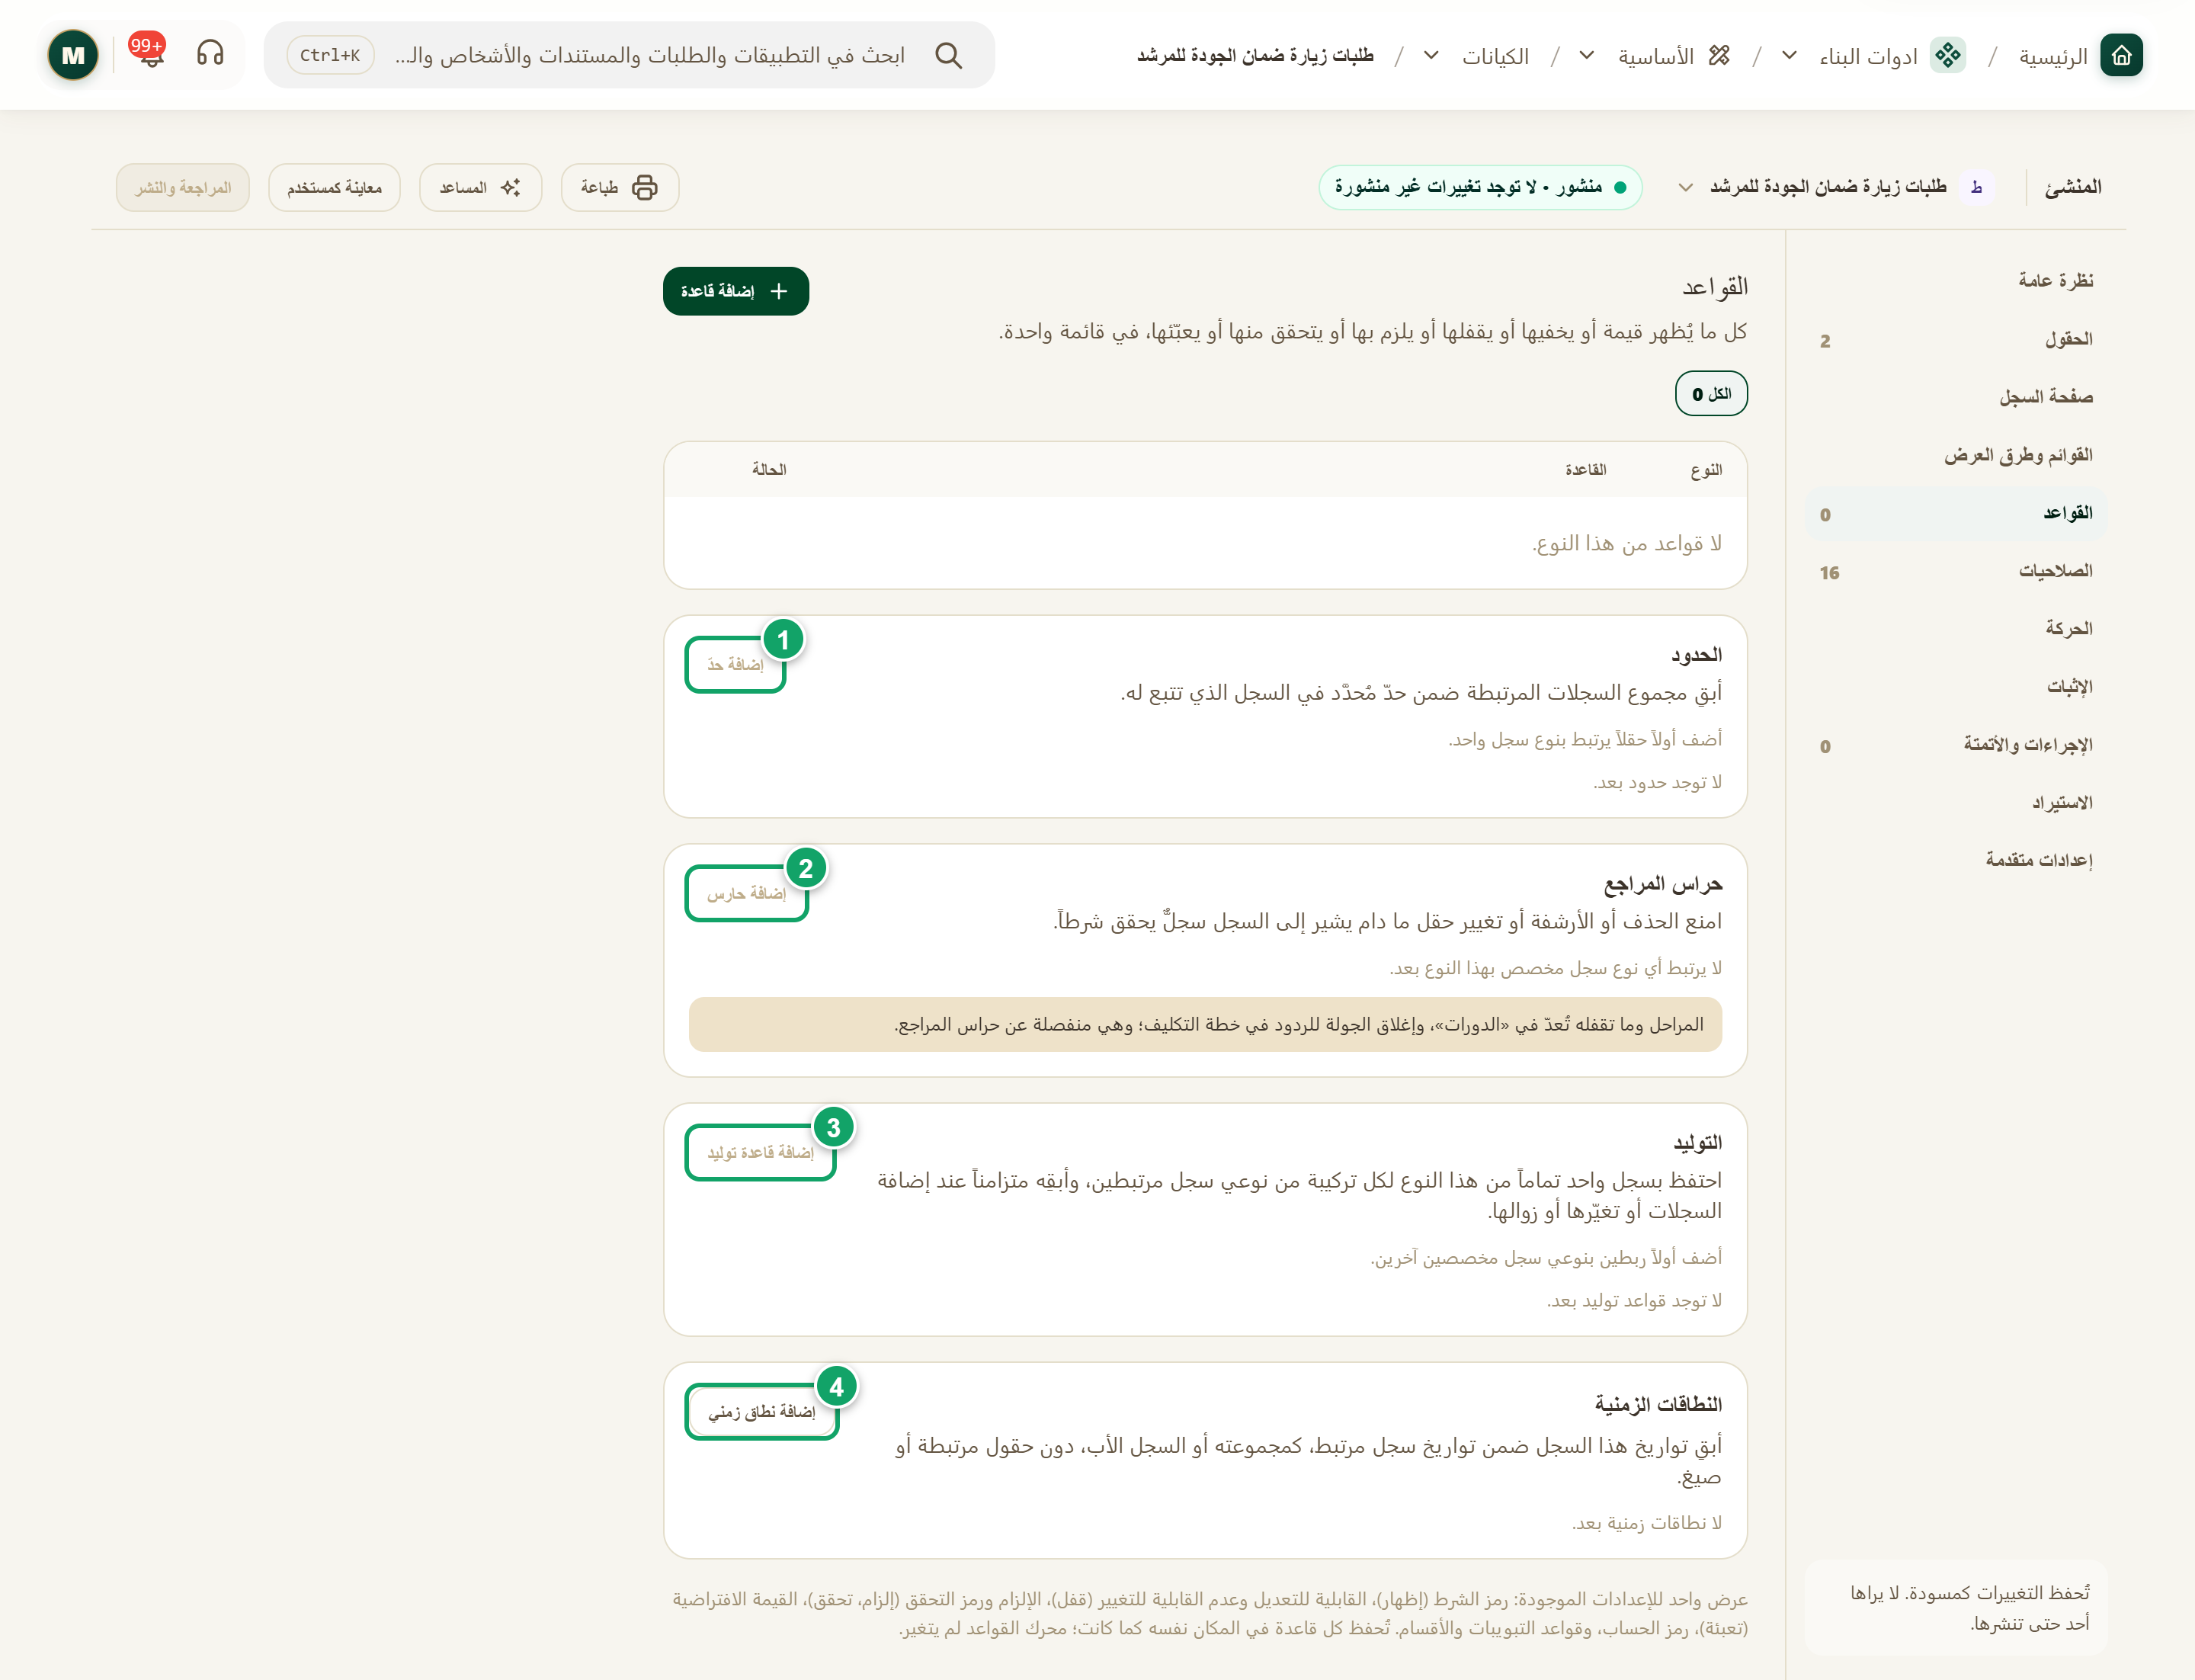
\includegraphics[width=0.95\linewidth,height=0.72\textheight,keepaspectratio]{figures/screens/ch06-ws-rule-tools-ar.png}
\caption{الأدوات الأربع أسفل جدول القواعد}
\label{fig:builder-record-limits-screen}
\shotnote{تعرض الصورة قسم «القواعد» في النوع الاختباري، وتحت جدول القواعد بطاقة لكل أداة مع زر الإضافة الخاص بها. وتظهر في كل بطاقة رسالة تبيّن ما يلزم قبل استخدامها، مثل حقل علاقة. ① «إضافة حدّ». ② «إضافة حارس». ③ «إضافة قاعدة توليد». ④ «إضافة نطاق زمني». ويبدأ كل زر محرراً يقودك إلى إكمال الجملة التي تصف الضابط.}
\end{figure}

\begin{table}[H]
\centering
\caption{الأدوات الأربع}
\label{tab:builder-record-limits-tools}
\begin{tabularx}{\linewidth}{R{3.6cm} Y}
\rcHeaderRow
\thh{الأداة} & \thh{ما تفعله وما تضبطه}\\
الحدود & تُبقي مجموع السجلات المرتبطة ضمن حد يحدده السجل الذي تتبع له، مثل مجموع بنود الصرف ضمن الموازنة. تضبط فيها «ما يُجمع» و«النطاق» و«الحدّ»، وما يحدث «عند التجاوز»: الرفض، أو التحذير مع طلب سبب يصل إلى أدوار تقرر فيه.\\
حراس المراجع & ترفض حذف السجل أو أرشفته أو تغيير حقل فيه ما دامت سجلات أخرى تشير إليه وتطابق شرطاً، مع رسالة توضح السبب. ويمكن إضافة عشرة حراس على الأكثر لكل نوع.\\
التوليد & يُبقي سجلاً واحداً من هذا النوع لكل تركيبة من سجلات نوعين مرتبطين، ويحدّثه عند تغيّرهما، مثل سجل تقييم لكل موظف في كل دورة. وتعرض «المعاينة» عدد السجلات، و«تعبئة الآن» تنشئ الناقص منها، ولا يعمل قبل نشر النوع.\\
النطاقات الزمنية & تُبقي تاريخي البداية والنهاية داخل تواريخ سجل مرتبط أو السجل الأم، وتحدد ما يحدث عند تغيّر تواريخه: السماح مع إظهار السجلات الخارجة، أو رفض التغيير. ويرى المستخدم في السجل عبارة مثل «بين … و…».\\
\end{tabularx}
\end{table}

\begin{figure}[H]
\centering
\begin{tikzpicture}[node distance=0.5cm]
\node[stepBox] (a) {\RL{تحديد الخطر على البيانات}};
\node[stepBox,below=of a] (b) {\RL{اختيار الأداة المناسبة}};
\node[stepBox,below=of b] (c) {\RL{ضبطها وكتابة رسالتها}};
\node[stepBox,below=of c] (d) {\RL{المعاينة أو التجربة}};
\node[stepBox,below=of d] (e) {\RL{المراجعة والنشر}};
\draw[flowsTo] (a) -- (b);
\draw[flowsTo] (b) -- (c);
\draw[flowsTo] (c) -- (d);
\draw[flowsTo] (d) -- (e);
\end{tikzpicture}
\rclegend
\caption{إضافة ضابط بين السجلات}
\label{fig:builder-record-limits-flow}
\shotnote{يبدأ المخطط بتحديد الخطر لا بالأداة، لأن كل أداة تعالج خطراً مختلفاً: تجاوز مبلغ، أو حذف سجل مستخدم، أو سجلات ناقصة، أو تواريخ متعارضة. وتأتي كتابة الرسالة مع الضبط لأن المستخدم الذي يُرفض تعديله يحتاج إلى سبب واضح ليعرف ما يفعل.}
\end{figure}

\subsection{خطوات العمل والتحقق}
\begin{enumerate}
\item حدد الخطر الذي تريد منعه، ثم افتح «القواعد» وانزل إلى الأداة المناسبة.
\item اضغط زر الإضافة في الأداة، مثل «إضافة حدّ»، وأكمل الجملة التي يعرضها المحرر خطوة بخطوة.
\item اكتب رسالة تشرح للمستخدم سبب الرفض وما يمكنه فعله.
\item استخدم «المعاينة» إن توفرت، ثم انشر التغييرات وجرّب الحالة الممنوعة بسجل تجريبي.
\end{enumerate}

\textbf{تحقق ومعالجة المشكلة:} يجب أن يُرفض التعديل الممنوع مع رسالتك، وأن يُقبل التعديل السليم. فإذا ظهر في «قبل النشر» أن إعدادات حدّ أو حارس أو توليد غير صالحة، فافتحها من زر الإصلاح وأكمل الحقل الناقص. وتذكّر أن التوليد يحتاج إلى نشر النوع قبل أن يعمل.

\clearpage
\section{الصلاحيات}
\label{sec:builder-feature-access}

تحدد الصلاحيات من يستطيع أن يفعل ماذا في سجلات هذا النوع. وتُسمّى هذه الأعمال «الأفعال»، مثل الرؤية في القوائم والفتح والإضافة والتغيير والحذف. ويعرض قسم «الصلاحيات» الأدوار والأفعال في جدول واحد، وهو يعدّل الأدوار نفسها الموجودة في الإعدادات ← الأدوار، فلا يُنشئ نظاماً ثانياً للصلاحيات.

\textbf{المسار ومن يستخدمه:} نوع السجلات ← «الصلاحيات». يستخدمه من يبني النوع ويملك صلاحية تحديث الأدوار.

\begin{rcnote}[مثال: شركة الأفق]
يمنح مسؤول النظام منسقي الفروع، ومنهم عمر حداد، فعلَي الإضافة والفتح في «طلبات الزيارة»، ويمنح مديرة الموارد البشرية سارة الخطيب فعل التغيير لتسجّل قرارها. ثم يتأكد من صلاحية عمر بالأداة ③.
\end{rcnote}

\begin{figure}[H]
\centering
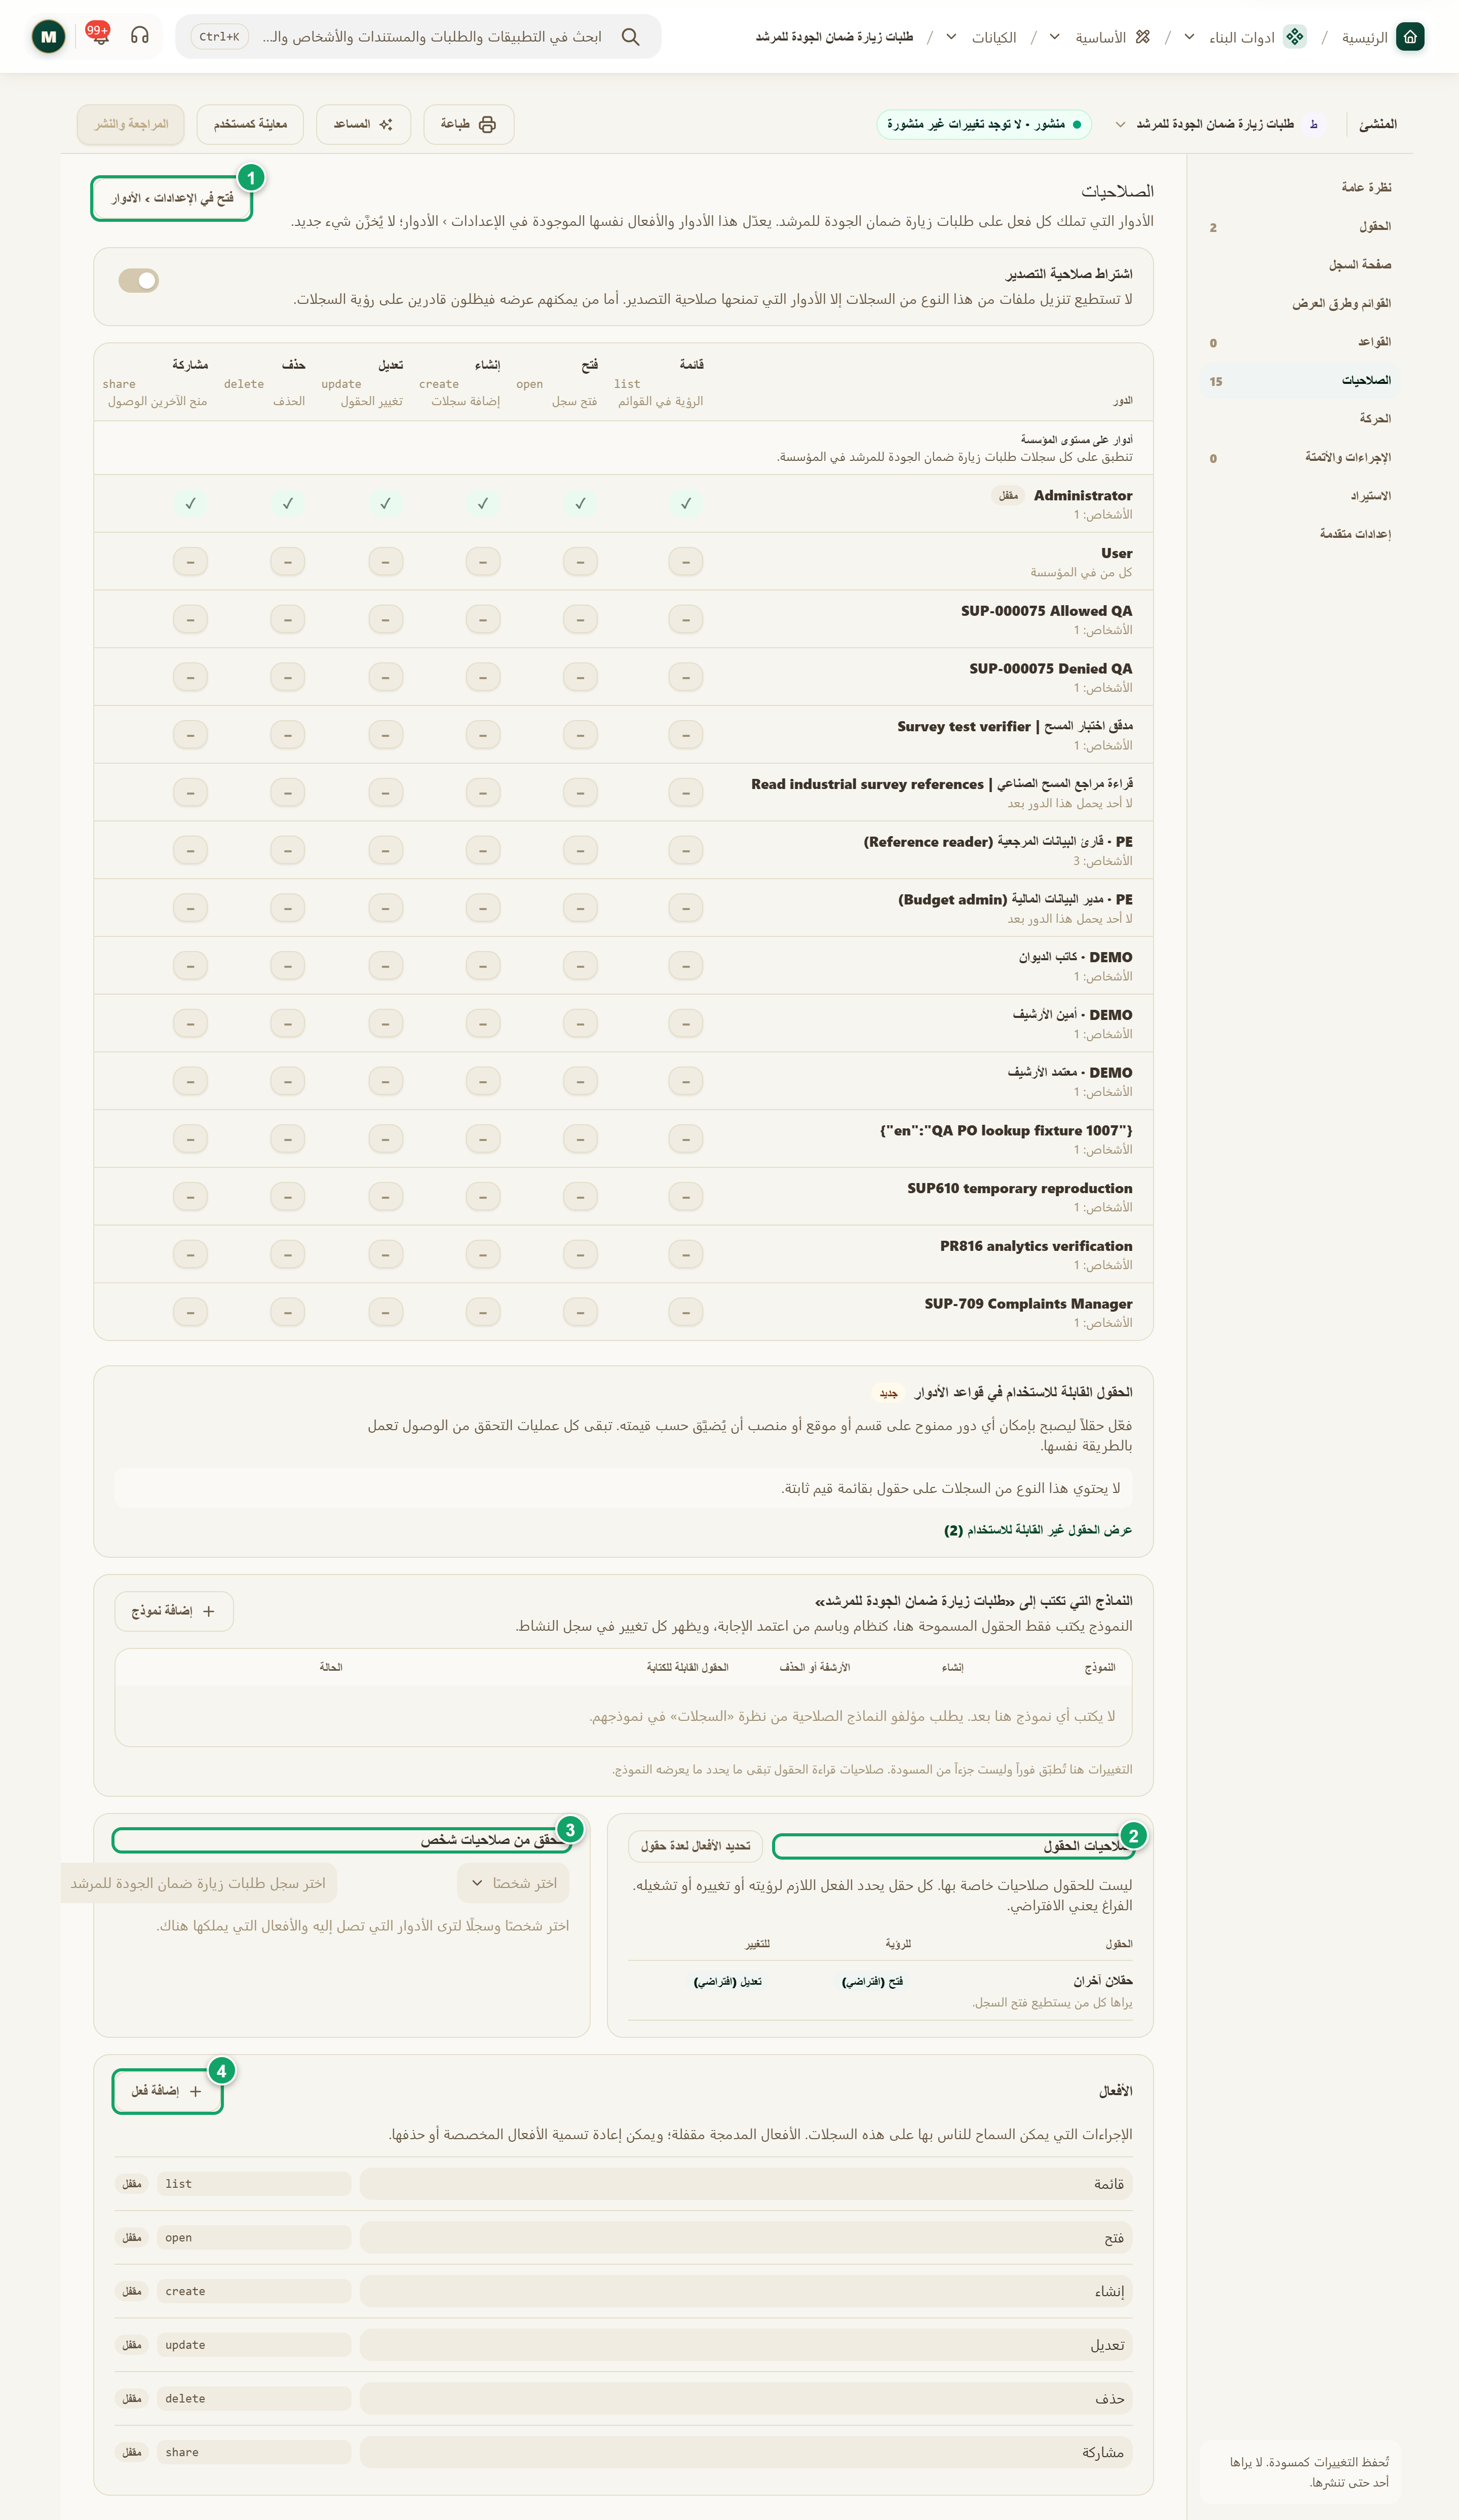
\includegraphics[width=0.95\linewidth,height=0.72\textheight,keepaspectratio]{figures/screens/ch06-ws-access-ar.png}
\caption{قسم «الصلاحيات»}
\label{fig:builder-access-screen}
\shotnote{يعرض القسم الأدوار والأفعال على هذا النوع، ثم صلاحيات الحقول وأداة فحص الوصول وقائمة الأفعال. والأدوار الظاهرة أدوار مؤسسة الاختبار. ① «فتح في الإعدادات › الأدوار». ② «صلاحيات الحقول»: تحدد الفعل اللازم لرؤية حقل أو تغييره. ③ «التحقق من صلاحيات شخص»: يبيّن ما يستطيعه شخص على سجل. ④ «إضافة فعل»: يضيف فعلاً مخصصاً مثل الاعتماد.}
\end{figure}


\begin{table}[H]
\centering
\caption{الأفعال المدمجة}
\label{tab:builder-access-verbs}
\begin{tabularx}{\linewidth}{R{3.6cm} Y}
\rcHeaderRow
\thh{الفعل} & \thh{ماذا يسمح به؟}\\
\en{list} & الرؤية في القوائم.\\
\en{open} & فتح سجل.\\
\en{create} & إضافة سجلات.\\
\en{update} & تغيير الحقول.\\
\en{delete} & الحذف.\\
\en{share} & منح الآخرين الوصول.\\
\en{export} & تنزيل ملف، ويظهر عند تفعيل «اشتراط صلاحية التصدير».\\
\end{tabularx}
\end{table}

\begin{table}[H]
\centering
\caption{ما الذي تجده هنا؟}
\label{tab:builder-access-data}
\begin{tabularx}{\linewidth}{R{3.6cm} Y}
\rcHeaderRow
\thh{البطاقة} & \thh{المحتوى والإجراء}\\
الأدوار والأفعال & اضغط الخانة لتمنح الدور فعلاً أو تسحبه. تظهر أدوار على مستوى المؤسسة، وأدوار على سجل واحد، وأدوار أخرى لها صلاحيات هنا.\\
صلاحيات الحقول & ليست للحقول صلاحيات خاصة؛ بل يحدد كل حقل الفعل اللازم «للرؤية» أو «للتغيير» أو «للتشغيل». الفراغ يعني الافتراضي.\\
الأفعال & «إضافة فعل» مخصص، مثل «اعتماد الميزانية»، ثم منحه للأدوار.\\
الحقول القابلة للاستخدام في قواعد الأدوار & تسمح بتضييق الدور حسب قيمة حقل، مثل الفرع.\\
اشتراط صلاحية التصدير & عند تفعيله لا ينزّل ملفات من هذا النوع إلا الأدوار التي تملك فعل \en{export}، ويبقى من يرى السجلات قادراً على رؤيتها.\\
النماذج التي تكتب إلى هذا النوع & تحدد النماذج المسموح لها بكتابة حقول هذا النوع. التغيير هنا يُطبّق فوراً، وليس جزءاً من المسودة.\\
التحقق من صلاحيات شخص & تختار شخصاً وسجلاً فترى الأدوار التي تصل إليه والأفعال التي يملكها.\\
\end{tabularx}
\end{table}

\begin{figure}[H]
\centering
\begin{tikzpicture}[node distance=0.5cm]
\node[entity] (role) {\RL{الدور}};
\node[entity,below=0.7cm of role] (verb) {\RL{الفعل}};
\node[entityOpt,below right=0.7cm and 0.3cm of verb] (field) {\RL{حقل يطلب الفعل}};
\node[entityOpt,below left=0.7cm and 0.3cm of verb] (records) {\RL{سجلات النوع}};
\draw[dependsOn] (role) -- (verb);
\draw[dependsOnOpt] (verb.south) -- ++(0,-0.3) -| (field.north);
\draw[dependsOnOpt] (verb.south) -- ++(0,-0.3) -| (records.north);
\end{tikzpicture}
\rclegend
\caption{من الدور إلى ما يستطيع الشخص فعله}
\label{fig:builder-access-model}
\shotnote{يوضّح الشكل أن الشخص لا يأخذ الصلاحية مباشرة، بل يأخذها من دوره، والدور يملك أفعالاً على سجلات النوع. ويمكن لحقل حساس أن يطلب فعلاً بعينه، فلا يراه أو يغيّره إلا من يملك ذلك الفعل. لذلك ابدأ بالأفعال المدمجة، ولا تضف فعلاً مخصصاً إلا لعمل له معنى مستقل مثل الاعتماد.}
\end{figure}

\subsection{خطوات العمل والتحقق}
\begin{enumerate}
\item افتح نوع السجلات واختر «الصلاحيات»، ثم راجع الأدوار الظاهرة.
\item اضغط الخانات لتمنح كل دور الأفعال التي يحتاجها عمله فقط.
\item للحقول الحساسة، افتح «صلاحيات الحقول» وحدد الفعل اللازم لرؤيتها أو تغييرها.
\item استخدم «التحقق من صلاحيات شخص» على موظف وسجل تجريبي، ثم انشر التغييرات.
\end{enumerate}

\textbf{تحقق ومعالجة المشكلة:} يجب أن تُظهر أداة التحقق الأفعال المتوقعة للشخص، وأن يرى المستخدم بعد النشر ما يخصه فقط. فإذا ظهرت رسالة «تحتاج فعل «تحديث» على الأدوار لتغيير الصلاحيات»، فاطلب ذلك من مسؤول المؤسسة؛ وإذا لم يظهر حقل لمستخدم، فراجع الفعل المطلوب له في «صلاحيات الحقول».

\clearpage
\section{صلاحيات الحقول والتحقق من صلاحيات شخص}
\label{sec:builder-feature-field-access}

تحدد صلاحيات النوع من يرى السجلات ومن يغيّرها، لكن بعض الحقول تحتاج إلى حماية أدق، مثل حقل المبلغ أو ملاحظات المراجع. وتشرح هذه الصفحة ثلاث بطاقات في قسم «الصلاحيات»: «صلاحيات الحقول» التي تحدد الفعل المطلوب لرؤية كل حقل وتغييره، و«الحقول القابلة للاستخدام في قواعد الأدوار» التي تضيّق الدور بقيمة في السجل، و«التحقق من صلاحيات شخص» التي تبيّن ما يراه شخص معيّن فعلاً.

\textbf{المسار ومن يستخدمه:} «المنشئ» ← «الصلاحيات». يستخدمه من يبني النوع بالتنسيق مع مسؤول الأدوار، لأن القسم يعدّل الأدوار والأفعال نفسها الموجودة في «الإعدادات» ← «الأدوار».

\begin{rcnote}[مثال: شركة الأفق]
يجعل المسؤول حقل «ملاحظات المراجعة» في «طلبات الزيارة» للقراءة فقط إلا لمن يملك فعل الاعتماد، ثم يستخدم «التحقق من صلاحيات شخص» مع عمر حداد وأحد طلباته، فيتأكد أن عمر يرى الملاحظات ولا يستطيع تغييرها.
\end{rcnote}

\begin{figure}[H]
\centering
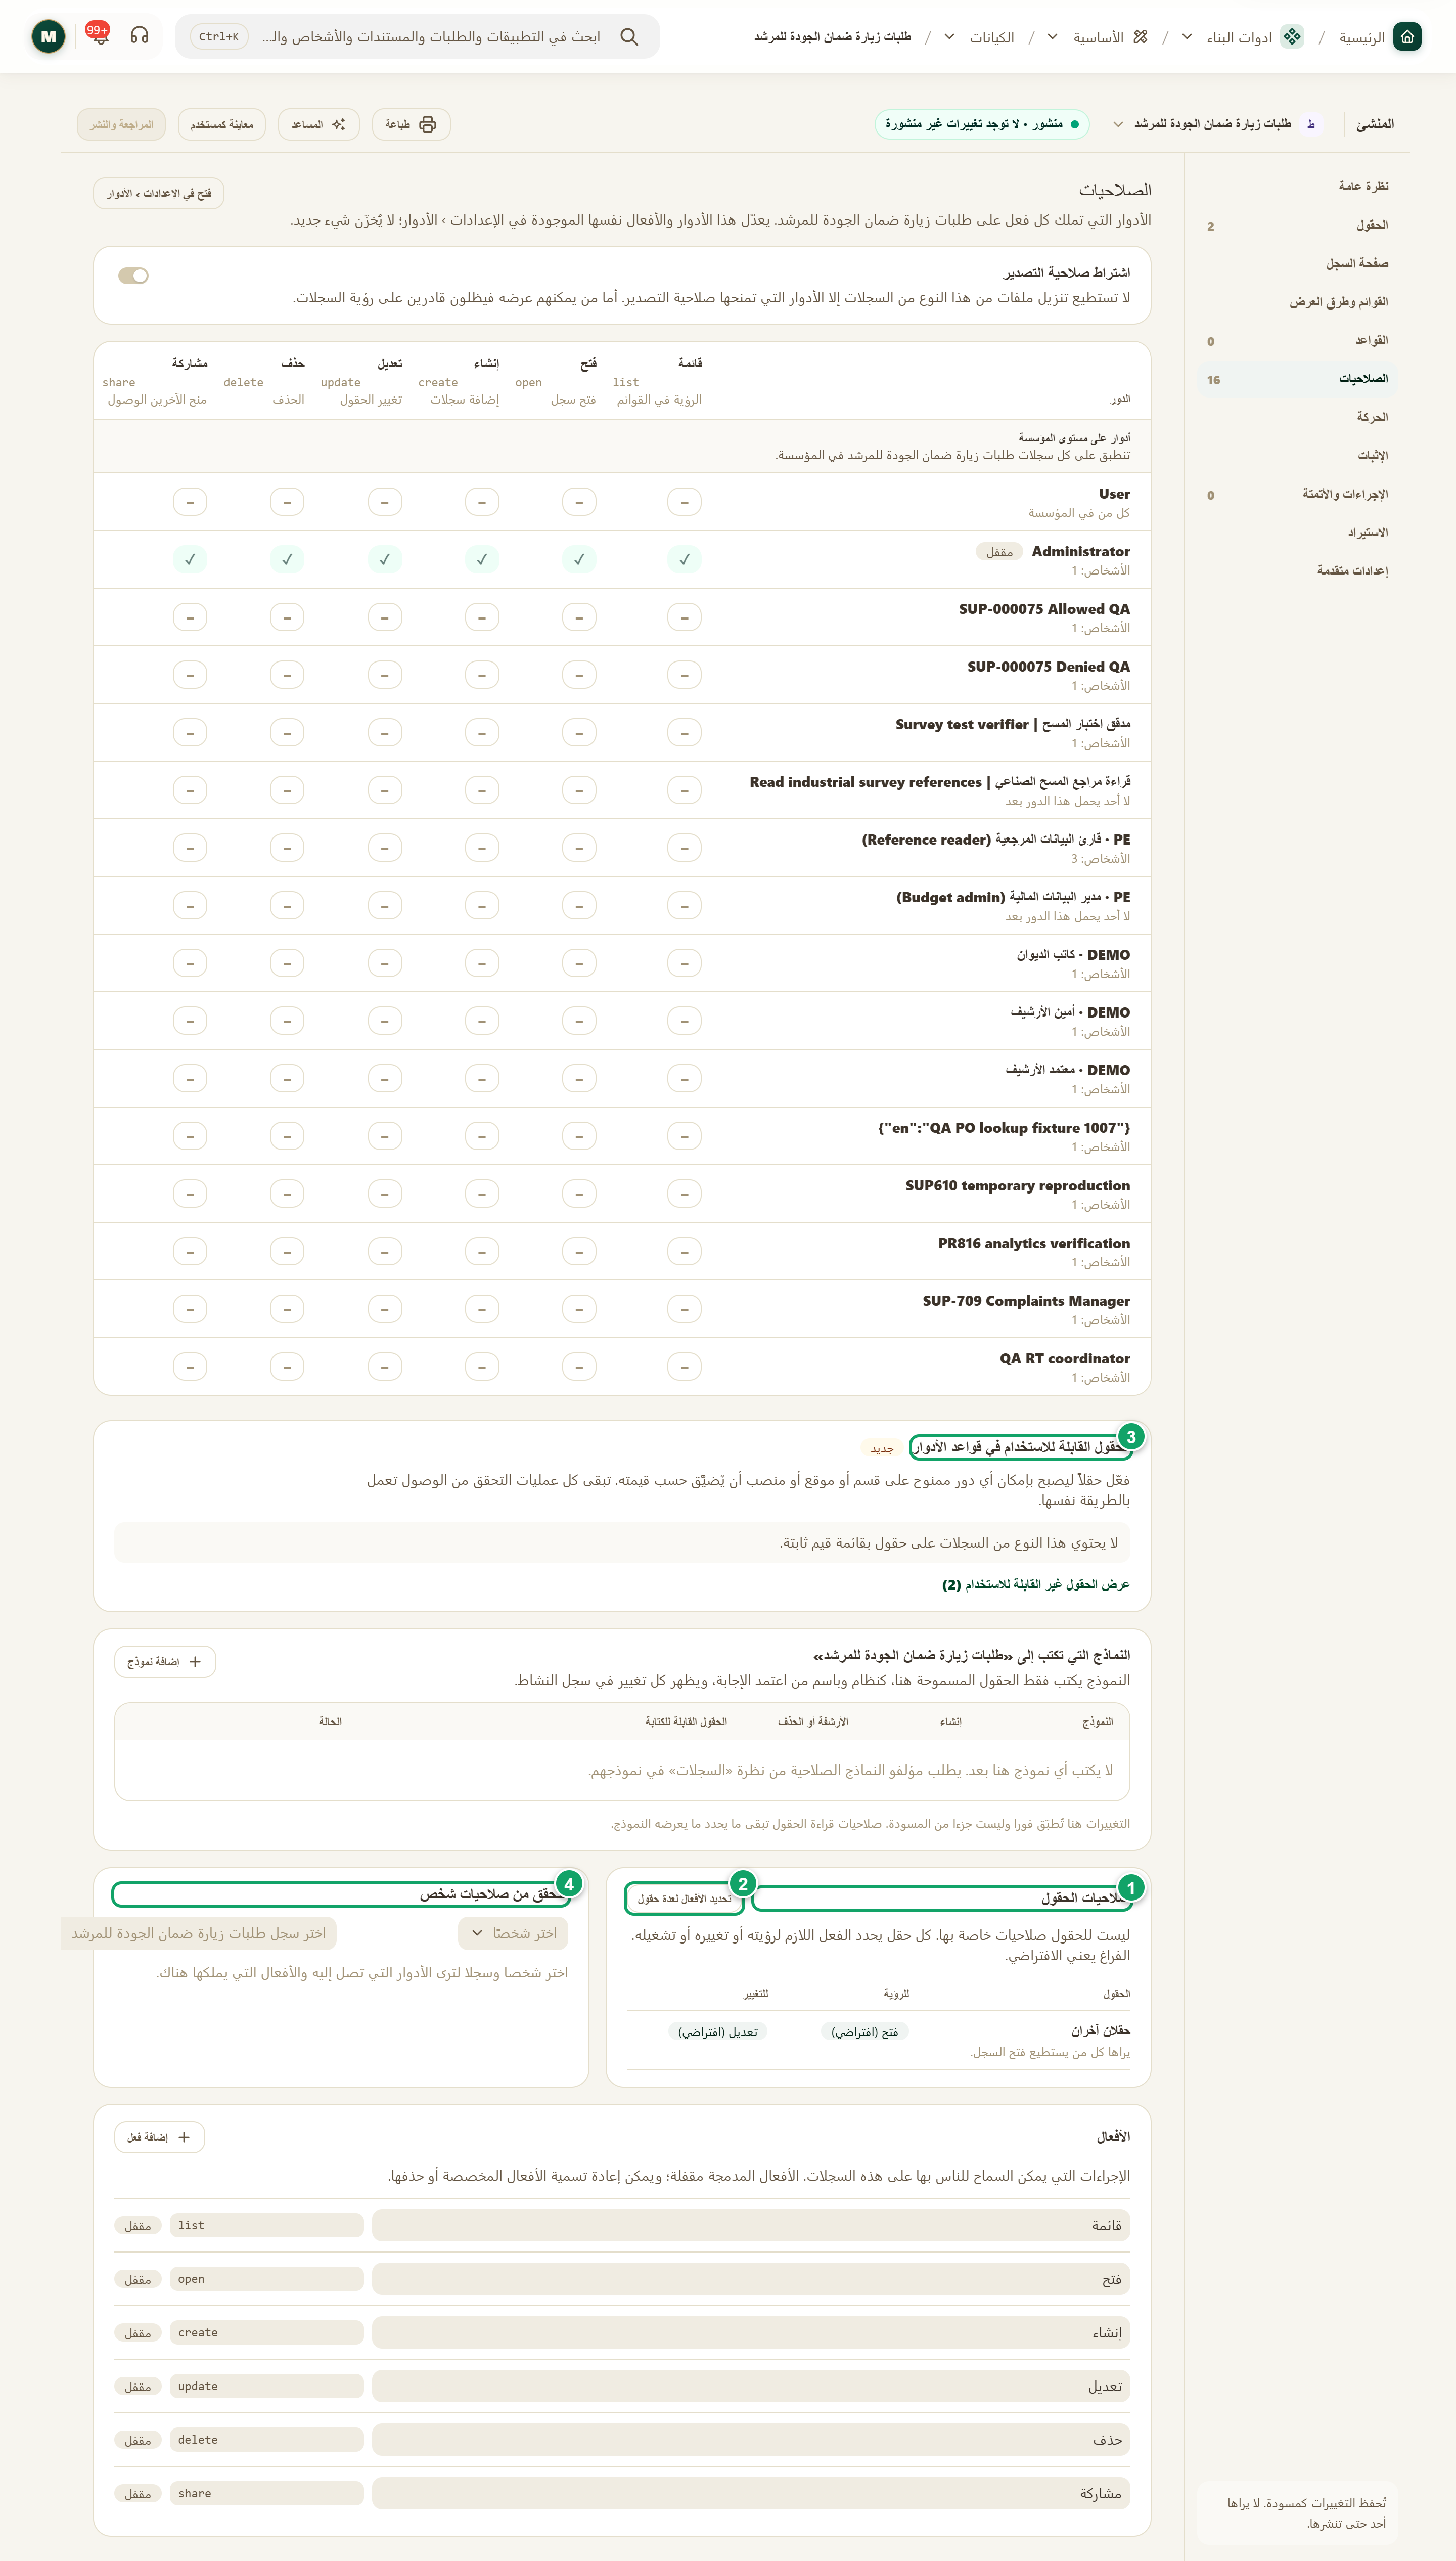
\includegraphics[width=0.95\linewidth,height=0.72\textheight,keepaspectratio]{figures/screens/ch06-ws-field-access-ar.png}
\caption{بطاقات الصلاحيات الدقيقة في قسم «الصلاحيات»}
\label{fig:builder-field-access-screen}
\shotnote{تعرض الصورة قسم «الصلاحيات» في النوع الاختباري كاملاً، ومنه البطاقات التي تضبط الحقول وتفحص ما يراه شخص معيّن. ويفيدك ذلك في معرفة ترتيبها على الصفحة قبل أن تبدأ. ① «صلاحيات الحقول»: جدول الفعل المطلوب لرؤية كل حقل وتغييره. ② «تحديد الأفعال لعدة حقول». ③ «الحقول القابلة للاستخدام في قواعد الأدوار»: تضيّق الدور بقيمة في السجل. ④ «التحقق من صلاحيات شخص»: يفحص ما يراه شخص في سجل.}
\end{figure}

\begin{table}[H]
\centering
\caption{بطاقات الصلاحيات الدقيقة}
\label{tab:builder-field-access-cards}
\begin{tabularx}{\linewidth}{R{3.6cm} Y}
\rcHeaderRow
\thh{البطاقة} & \thh{ما تقدمه}\\
صلاحيات الحقول & جدول بالحقول، لكل حقل عمودان: «للرؤية» و«للتغيير». تختار في كل منهما الفعل المطلوب، أو تتركه فارغاً ليتبع الصلاحية الافتراضية للسجل. ويعرض كل صف من يُخفى عنه الحقل ومن يراه للقراءة فقط.\\
تحديد الأفعال لعدة حقول & تختار عدة حقول وتضبط لها «للرؤية» و«للتغيير» معاً: الإبقاء على الحالي، أو الافتراضي، أو فعل معيّن، أو النظام وحده. ثم تضغط «تطبيق»، فيذهب التغيير إلى المسودة.\\
الحقول القابلة للاستخدام في قواعد الأدوار & تفعّل حقل علاقة أو قائمة أو نعم/لا، فيصبح ممكناً أن يُضيَّق الدور الممنوح على وحدة أو موقع أو منصب بقيمة هذا الحقل. ولا تصلح لذلك حقول النص والأرقام والتواريخ والحقول متعددة القيم، ويُقفل الحقل الذي تستخدمه الأدوار.\\
التحقق من صلاحيات شخص & تختار شخصاً وسجلاً، فترى الأدوار التي تصل إلى السجل، والأفعال التي يملكها، مع شطب ما لا يملكه، وعدد الحقول المخفية عنه أو المقروءة فقط. والفحص يعتمد على صلاحيات المسودة، فتتحقق قبل النشر.\\
\end{tabularx}
\end{table}

\begin{figure}[H]
\centering
\begin{tikzpicture}[node distance=0.5cm]
\node[stepBox] (a) {\RL{الأفعال على النوع}};
\node[stepBox,below=of a] (b) {\RL{صلاحيات الحقول}};
\node[stepBox,below=of b] (c) {\RL{التحقق من صلاحيات شخص}};
\node[stepBox,below=of c] (d) {\RL{المراجعة والنشر}};
\draw[flowsTo] (a) -- (b);
\draw[flowsTo] (b) -- (c);
\draw[flowsTo] (c) -- (d);
\end{tikzpicture}
\rclegend
\caption{ضبط صلاحيات الحقول والتأكد منها}
\label{fig:builder-field-access-flow}
\shotnote{يبدأ المخطط بأفعال النوع لأن صلاحية الحقل تُكتب بفعل منها، فلا معنى لها قبل أن تُمنح الأدوار أفعالها. ويضع التحقق من شخص بعينه قبل النشر، لأن الفحص يقرأ المسودة، فتكتشف الحقل المكشوف أو المخفي بالخطأ قبل أن يصل إلى الفريق.}
\end{figure}

\subsection{خطوات العمل والتحقق}
\begin{enumerate}
\item افتح «الصلاحيات»، وتأكد أن الأدوار تملك الأفعال الأساسية على النوع، مثل الفتح والتغيير.
\item في «صلاحيات الحقول» اختر للحقل الحساس الفعل المطلوب في «للرؤية» أو «للتغيير»، أو استخدم «تحديد الأفعال لعدة حقول» لعدة حقول معاً.
\item في «التحقق من صلاحيات شخص» اختر موظفاً وسجلاً، وراجع الحقول المخفية عنه والمقروءة فقط.
\item انشر التغييرات، ثم اطلب من الموظف أن يفتح السجل ويتأكد مما يراه.
\end{enumerate}

\textbf{تحقق ومعالجة المشكلة:} يجب أن يطابق ما يراه الموظف نتيجة الفحص. فإذا ظهر «لا يستطيع هذا الشخص فتح السجل»، فالمشكلة في أفعال النوع أو في دوره، لا في صلاحيات الحقول؛ فراجع الأدوار التي تصل إلى السجل أولاً.

\clearpage
\section{الإجراءات والأتمتة}
\label{sec:builder-feature-actions}

الإجراء زر يظهر في السجل، يُنشئ مستند Word أو جدول بيانات من بيانات السجل، أو يفتح رابطاً، أو يبدأ مسار عمل. ويجمع هذا القسم أزرار النوع، ويعرض الأتمتة المرتبطة به، والحقول المحسوبة التي يعيد النظام حسابها دورياً.

\textbf{المسار ومن يستخدمه:} نوع السجلات ← «الإجراءات والأتمتة». يستخدمه من يبني النوع بعد تجهيز القالب أو مسار العمل الذي سيستدعيه الزر.

\begin{rcnote}[مثال: شركة الأفق]
يضيف مسؤول النظام إلى طلب الزيارة زراً من نوع «مستند Word» يُنشئ خطاب تأكيد الزيارة من بيانات الطلب، ويجعله متاحاً لمن يملك فعل الاعتماد فقط. ويبدأ الزر من ①.
\end{rcnote}

\begin{figure}[H]
\centering
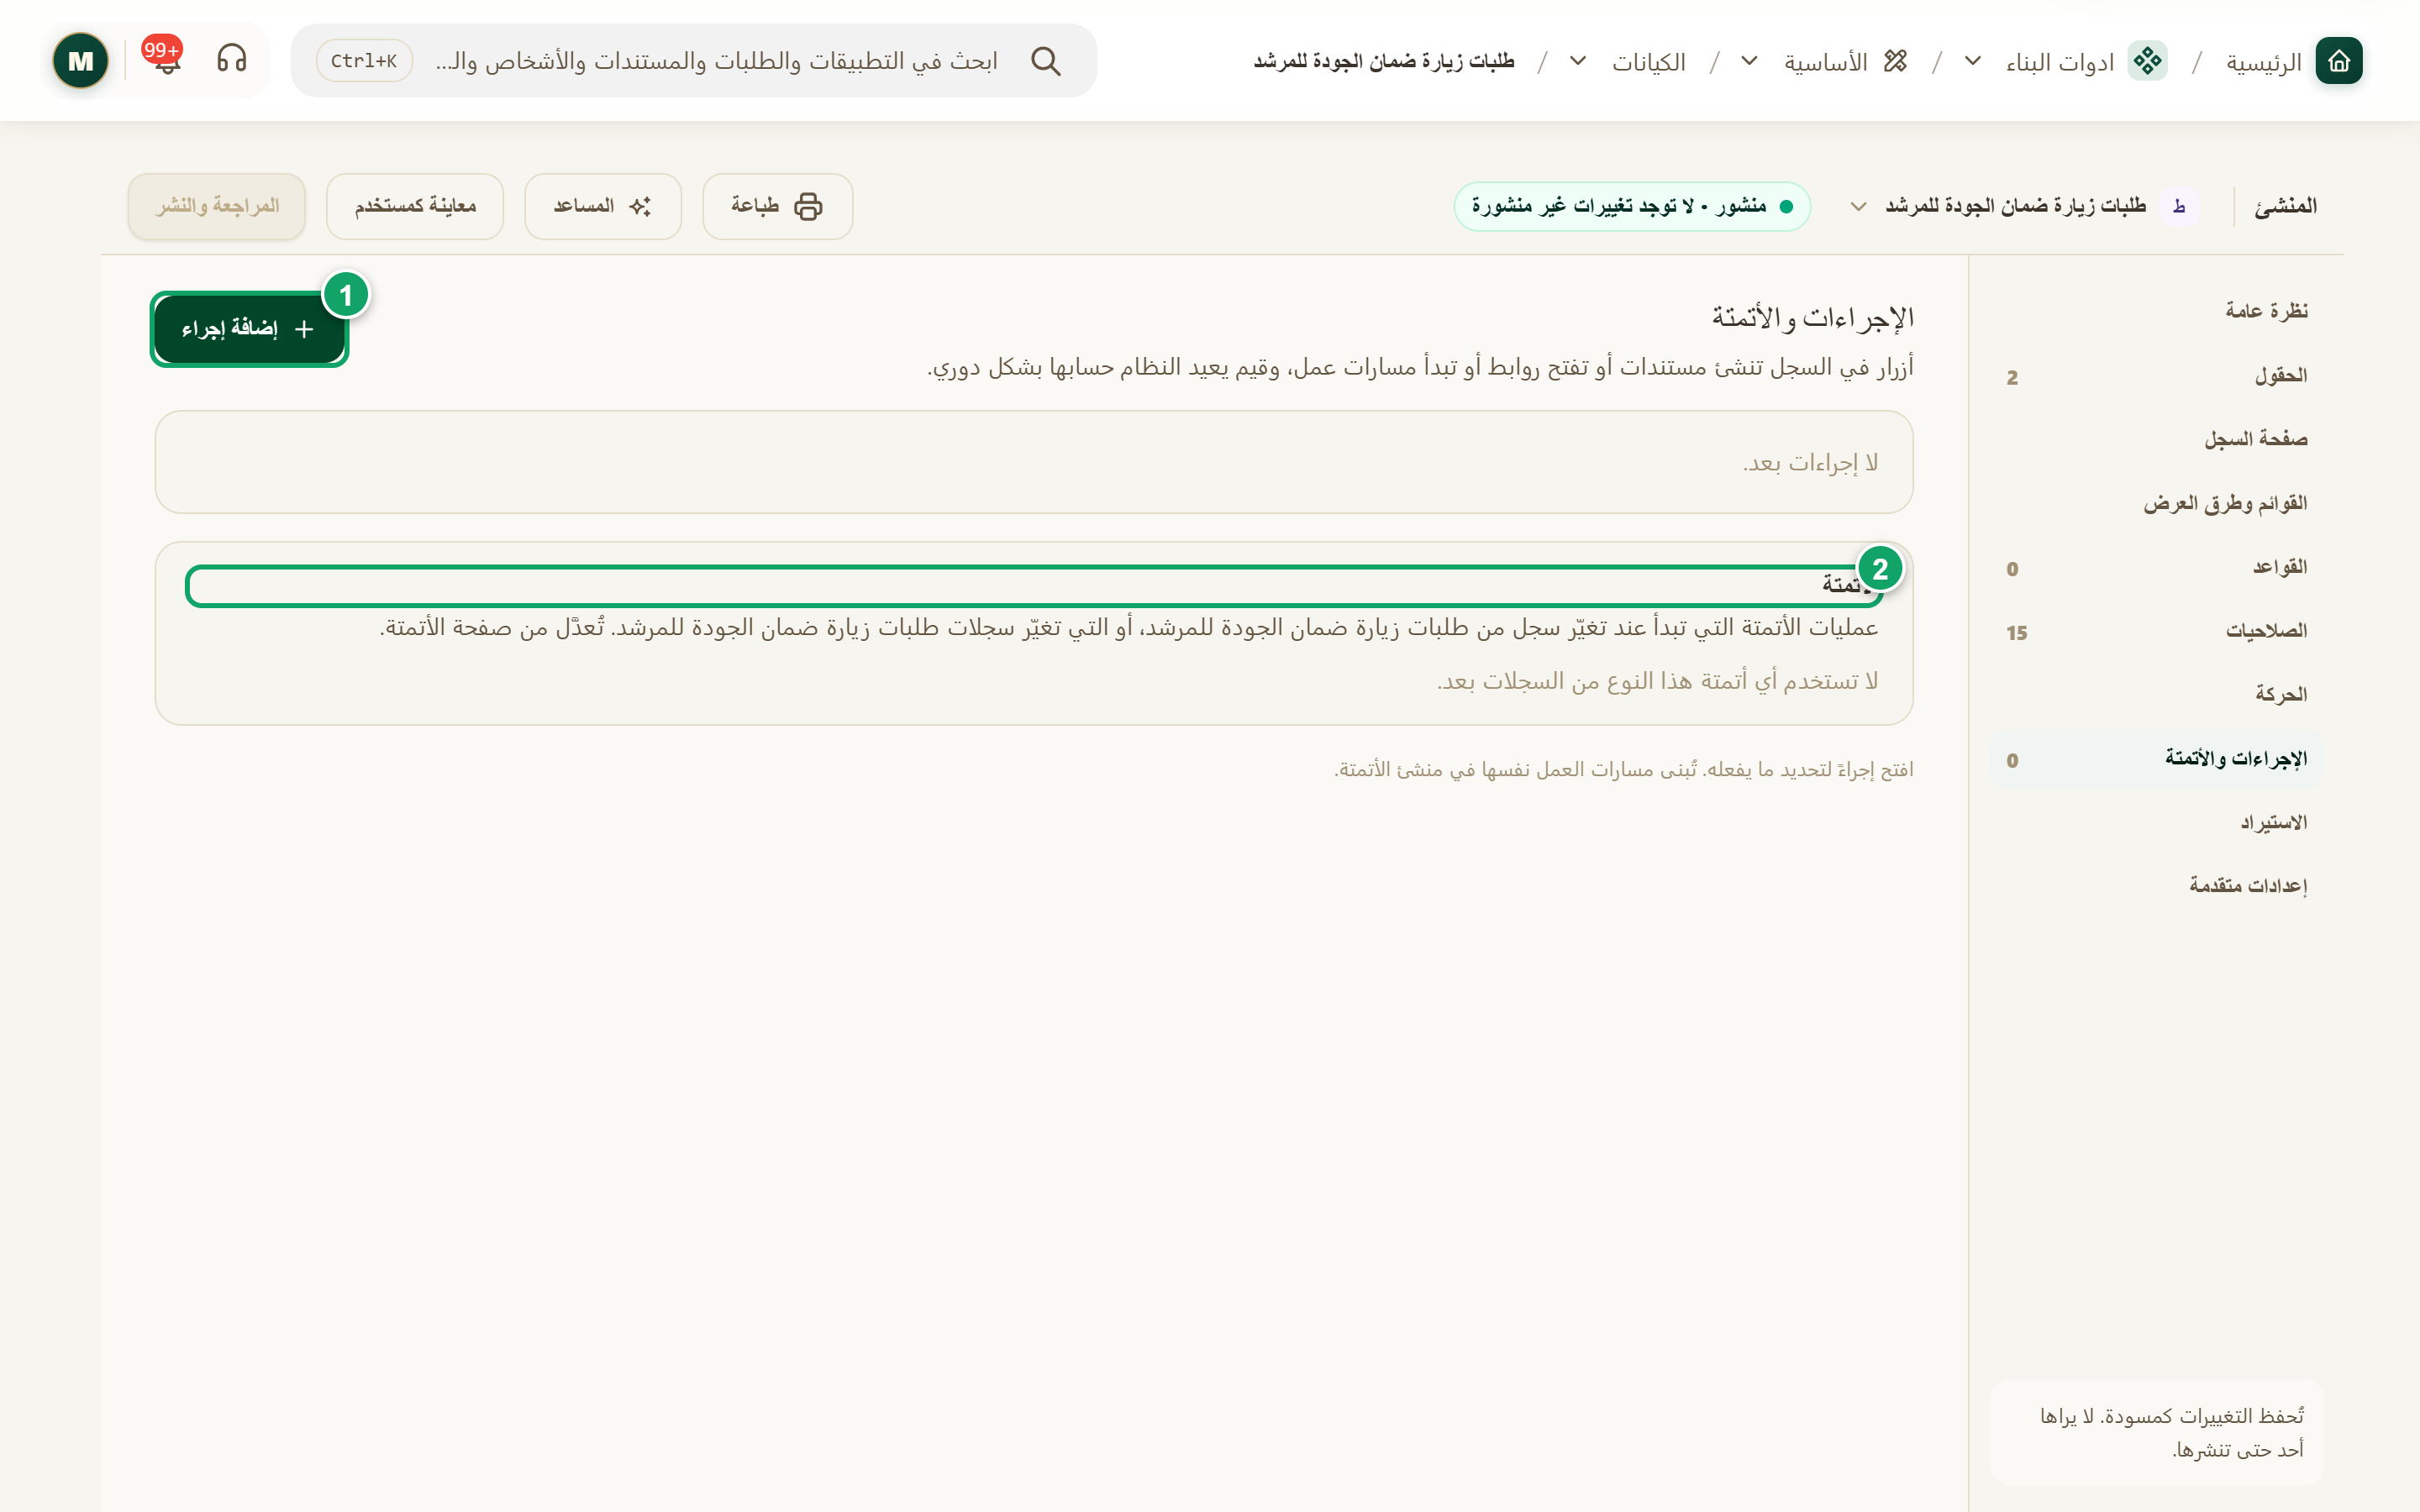
\includegraphics[width=0.95\linewidth,height=0.72\textheight,keepaspectratio]{figures/screens/ch06-ws-actions-ar.png}
\caption{قسم «الإجراءات والأتمتة»}
\label{fig:builder-actions-screen}
\shotnote{يعرض القسم أزرار النوع والأتمتة المرتبطة به، وهما فارغان في النوع الاختباري. ① «إضافة إجراء»: يُنشئ زراً جديداً ويفتحه لتحدد ما يفعله. ② «الأتمتة»: قائمة للاطلاع على الأتمتة التي تبدأ بتغيّر سجلات النوع أو تغيّرها.}
\end{figure}


\begin{table}[H]
\centering
\caption{ما الذي تجده هنا؟}
\label{tab:builder-actions-data}
\begin{tabularx}{\linewidth}{R{3.6cm} Y}
\rcHeaderRow
\thh{الجزء} & \thh{المحتوى والإجراء}\\
الإجراءات & لكل إجراء نوعه: «مستند Word» أو «جدول بيانات» أو «رابط» أو «مسار عمل»، ومن يستطيع تشغيله: «يتطلب» فعلاً معيناً، أو «كل من يستطيع تغيير السجل».\\
إضافة إجراء & يُنشئ «إجراء جديد» في المسودة ويفتحه في «الحقول»، حيث تختار ما يفعله والقالب أو المسار الذي يستخدمه.\\
الأتمتة & قائمة للاطلاع بالأتمتة التي «تبدأ عند التغيير» في سجل من هذا النوع، أو التي «تغيّر السجلات»، مع حالتها: «منشورة» أو «غير منشورة» أو «متوقفة مؤقتًا». تُعدَّل من صفحة الأتمتة.\\
يُعاد حسابه دوريًا & الحقول المحسوبة التي يعيد النظام حسابها «يوميًا» أو «أسبوعيًا» أو «شهريًا»، وتظهر عند وجودها فقط.\\
\end{tabularx}
\end{table}

\begin{figure}[H]
\centering
\begin{tikzpicture}[node distance=0.5cm]
\node[entity] (action) {\RL{زر الإجراء في السجل}};
\node[entityOpt,below right=0.7cm and 0.3cm of action] (tpl) {\RL{قالب مستند}};
\node[entityOpt,below left=0.7cm and 0.3cm of action] (sop) {\RL{مسار عمل}};
\draw[dependsOnOpt] (action.south) -- ++(0,-0.3) -| (tpl.north);
\draw[dependsOnOpt] (action.south) -- ++(0,-0.3) -| (sop.north);
\end{tikzpicture}
\rclegend
\caption{ما يستدعيه الإجراء}
\label{fig:builder-actions-model}
\shotnote{يوضّح الشكل أن الزر لا يعمل وحده، بل يستدعي شيئاً جاهزاً: قالب مستند تُعدّه في صفحات القوالب، أو مسار عمل تبنيه في الأتمتة. لذلك جهّز القالب أو المسار أولاً، ثم أنشئ الإجراء واربطه به.}
\end{figure}

\subsection{خطوات العمل والتحقق}
\begin{enumerate}
\item جهّز القالب أو مسار العمل الذي سيستدعيه الزر.
\item افتح نوع السجلات واختر «الإجراءات والأتمتة»، ثم اضغط «إضافة إجراء».
\item في الحقل الذي يُفتح، سمِّ الإجراء واختر نوعه والقالب أو المسار، ثم حدد الفعل اللازم لتشغيله.
\item انشر التغييرات، ثم افتح سجلاً تجريبياً واضغط الزر.
\end{enumerate}

\textbf{تحقق ومعالجة المشكلة:} يجب أن يظهر الزر في السجل لمن يملك الفعل المطلوب، وأن ينتج المستند أو يبدأ المسار. فإذا ظهر الإجراء بنوع «غير مضبوط»، فافتحه وأكمل اختيار ما يفعله؛ وإذا لم يظهر الزر لمستخدم، فراجع الفعل الذي يتطلبه.

\clearpage
\section{الحركة}
\label{sec:builder-feature-movement}

الحركة إعداد متخصص لسجلات تنقل مبلغاً أو كمية من سجل إلى آخر، مثل التحويل بين بنود الموازنة أو بين المستودعات. فكل سجل يحدد من أين يأتي المبلغ وإلى أين يذهب، ويحافظ كيان على تساوي الطرفين، ويرحّلهما معاً عندما يصل السجل إلى حالة تختارها. ولا تحتاج معظم أنواع السجلات إلى هذا القسم. وإذا شغّلت «الإثبات» على النوع نفسه، فيجب أن ترحّل الحركة عند حالة التدقيق، كما تشرح الصفحة \ref{sec:builder-feature-evidence}.

\textbf{المسار ومن يستخدمه:} نوع السجلات ← «الحركة». يستخدمه من يبني أنواع سجلات مالية أو مخزنية.

\begin{rcnote}[مثال: شركة الأفق]
لا يحتاج نوع «طلبات الزيارة» إلى الحركة. لكن لو أنشأت الأفق نوعاً لتحويل مبالغ بين بنود موازنة الفروع، فسيرحّل كل تحويل معتمد المبلغ من بند حلب إلى بند دمشق في خطوة واحدة. ولا يتجاوز مسؤول النظام شروط ② لأن نوع الطلبات لا يحتاج إليها.
\end{rcnote}

\begin{figure}[H]
\centering
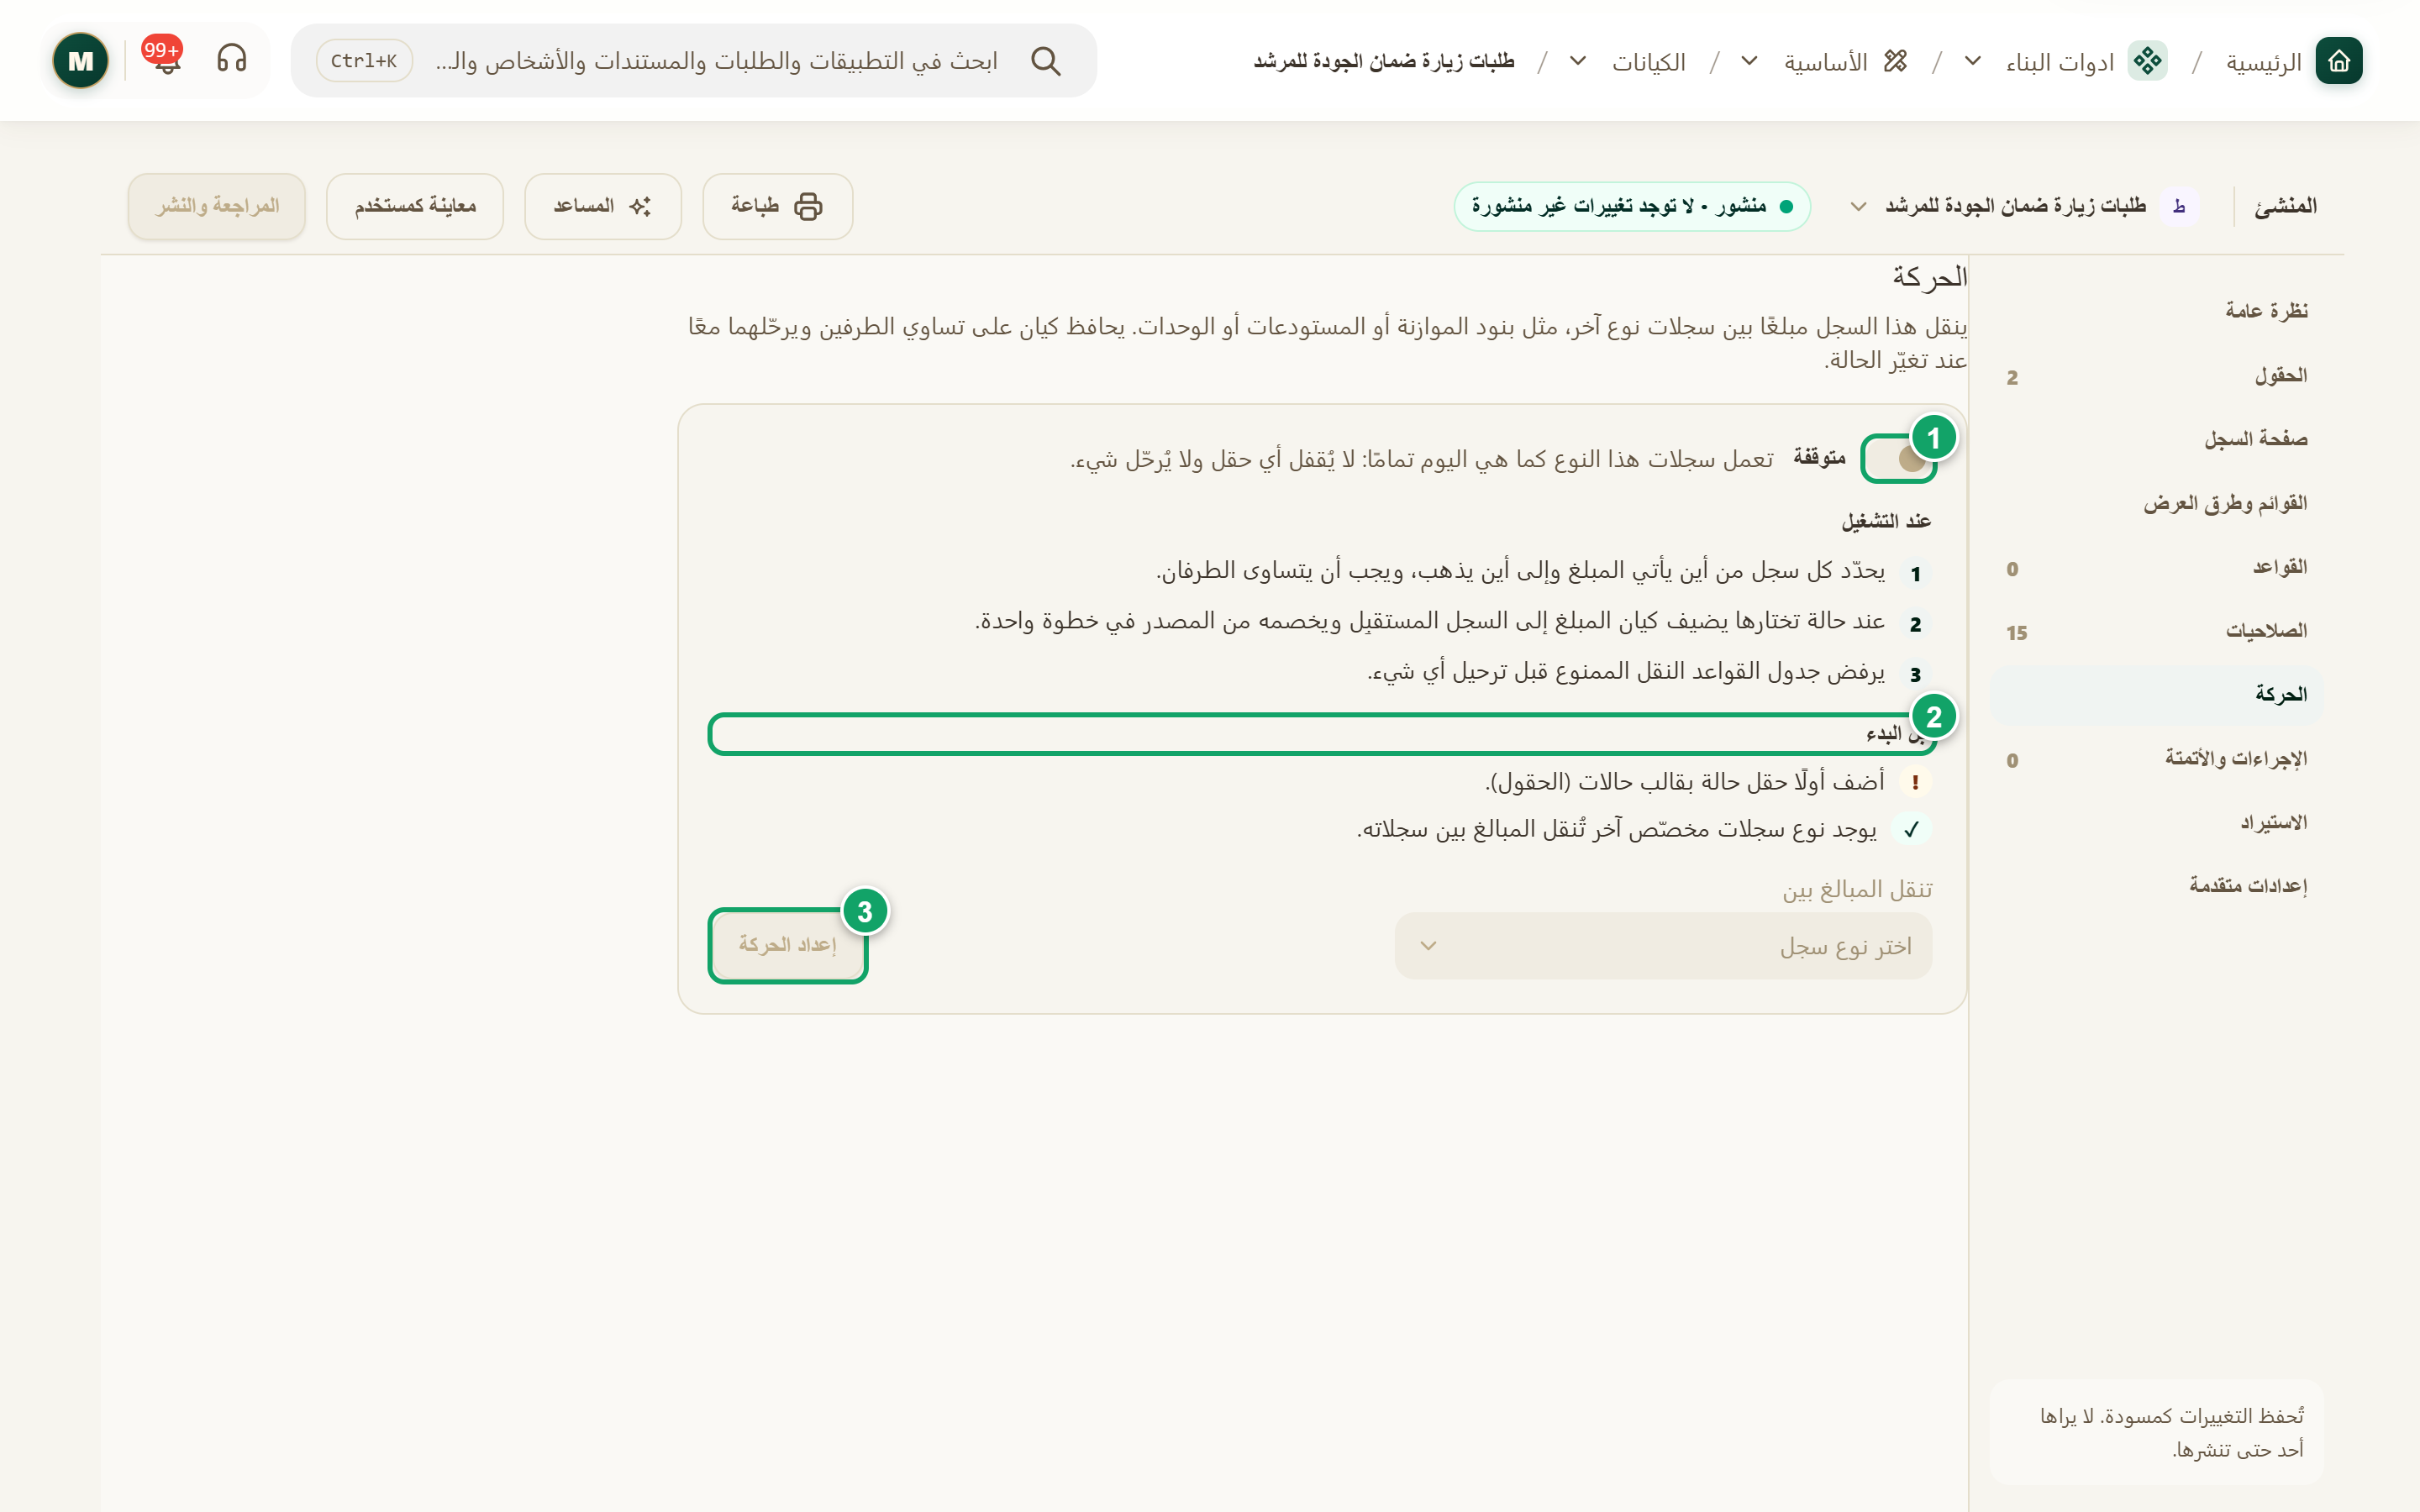
\includegraphics[width=0.95\linewidth,height=0.72\textheight,keepaspectratio]{figures/screens/ch06-ws-movement-ar.png}
\caption{قسم «الحركة» وهي متوقفة}
\label{fig:builder-movement-screen}
\shotnote{يشرح القسم ما تفعله الحركة عند تشغيلها، ويتحقق من شروطها قبل البدء. وتظهر علامة التنبيه لأن النوع الاختباري بلا حقل حالة. ① مفتاح التشغيل: متوقف، فلا يُرحَّل شيء. ② «قبل البدء»: الشروط الواجب توفرها، مع علامة لكل شرط. ③ «إعداد الحركة»: يبدأ الإعداد بعد اختيار النوع الذي تُنقل المبالغ بين سجلاته.}
\end{figure}


\begin{table}[H]
\centering
\caption{ما الذي تحتاجه وتضبطه؟}
\label{tab:builder-movement-data}
\begin{tabularx}{\linewidth}{R{3.6cm} Y}
\rcHeaderRow
\thh{الجزء} & \thh{المعنى}\\
قبل البدء & حقل «الحالة» بقالب حالات في هذا النوع، ونوع سجلات مخصّص آخر تُنقل المبالغ بين سجلاته، فيه حقلان رقميان لـ«الوارد» و«الصادر». ولا تعمل الحركة على الأنواع المدمجة.\\
الطرفان & من أين يأتي المبلغ وإلى أين يذهب، ويجب أن يتساويا.\\
الترحيل & الحالة التي يُرحَّل عندها المبلغ، وأثرها: حجز أو ترحيل أو فكّ الحجز أو عكس.\\
القواعد & ترفض النقل الممنوع قبل ترحيل أي شيء.\\
المجاميع الدورية وجرّب & تعرض المجاميع لكل فترة، وتختبر الإعداد قبل النشر.\\
\end{tabularx}
\end{table}

\begin{figure}[H]
\centering
\begin{tikzpicture}[node distance=0.5cm]
\node[stepBox] (a) {\RL{سجل الحركة: مسودة}};
\node[stepBox,below=of a] (b) {\RL{الوصول إلى حالة الترحيل}};
\node[stepBox,below=of b] (c) {\RL{خصم من المصدر وإضافة للمستقبِل}};
\draw[flowsTo] (a) -- (b);
\draw[flowsTo] (b) -- (c);
\end{tikzpicture}
\rclegend
\caption{متى يتحرك المبلغ؟}
\label{fig:builder-movement-flow}
\shotnote{يبيّن المخطط أن المبلغ لا يتحرك عند إنشاء السجل، بل عندما يصل إلى الحالة التي اخترتها للترحيل. وعندها يُخصم من المصدر ويُضاف إلى المستقبِل معاً، فلا يبقى طرف دون الآخر.}
\end{figure}

\subsection{خطوات العمل والتحقق}
\begin{enumerate}
\item تأكد من وجود حقل «الحالة» ونوع السجلات المستقبِل بحقلي الوارد والصادر.
\item افتح «الحركة»، واختر النوع من «تنقل المبالغ بين»، ثم اضغط «إعداد الحركة».
\item اضبط تبويبات «الطرفان» و«الترحيل» و«القواعد»، ثم استخدم «جرّب» قبل النشر.
\end{enumerate}

\textbf{تحقق ومعالجة المشكلة:} بعد النشر انقل سجلاً تجريبياً إلى حالة الترحيل، وتأكد من تغيّر رصيدي الطرفين بالمقدار نفسه. وإذا أوقفت الحركة لاحقاً، فتبقى المبالغ المرحّلة كما هي، ويتوقف ترحيل السجلات الجديدة فقط.

\clearpage
\section{الإثبات}
\label{sec:builder-feature-evidence}

«الإثبات» قسم متخصص لأنواع السجلات التي تسجّل مبلغاً صُرف أو قُبض، مثل مطالبات المصاريف، ويجب أن تثبته وثائق. ويسمّي القسم كل سجل من هذا النوع «قيداً»: يرفق مقدّمه الوثائق المطلوبة ثم يقدّمه، فيفحص كيان الوثائق والتكرار ويرقّم القيد ويجمّد ملفاته. ثم يجيب مدقق عن قائمة تحقق لكل وثيقة، ولا يكون المدقق منشئ القيد ولا مقدّمه. وبعد التدقيق يُقفل القيد على الجميع، ويكون التصحيح بقيد عكسي لا بالتعديل.

يبدأ القسم بحالة «متوقف»، فتعمل السجلات كما هي دون فحص أي ملف. ولا يعمل زر «تشغيل» إلا بشرطين يعرضهما القسم في «قبل أن تبدأ»: حقل حالة بقالب حالات، وحقل رقمي للمبلغ. ولا يتاح الإثبات لأنواع السجلات المدمجة في النظام.

\textbf{المسار ومن يستخدمه:} «المنشئ» ← «الإثبات». يضبطه من يبني الأنواع المالية بالتنسيق مع المسؤول المالي. وبعد النشر يظهر في صفحة السجل تبويب «الإثبات»، فيرفع فيه المقدّم الوثائق ويضغط «تقديم للتدقيق»، ويدقق فيه المدقق القيد أو يعيده للتصحيح.

\begin{rcnote}[مثال: شركة الأفق]
لا يحتاج نوع «طلبات الزيارة» إلى الإثبات لأنه لا يسجّل مبلغاً. لكن لو أنشأت الأفق نوعاً لمصاريف الزيارات، لجعل مسؤول النظام فيه وثيقة «فاتورة الفندق» مطلوبة دائماً، مع بند تحقق «الفاتورة باسم الشركة». فيرفع عمر حداد فاتورة زيارته إلى فرع حلب ويقدّم القيد، ثم تدققه سارة الخطيب.
\end{rcnote}

\begin{figure}[H]
\centering
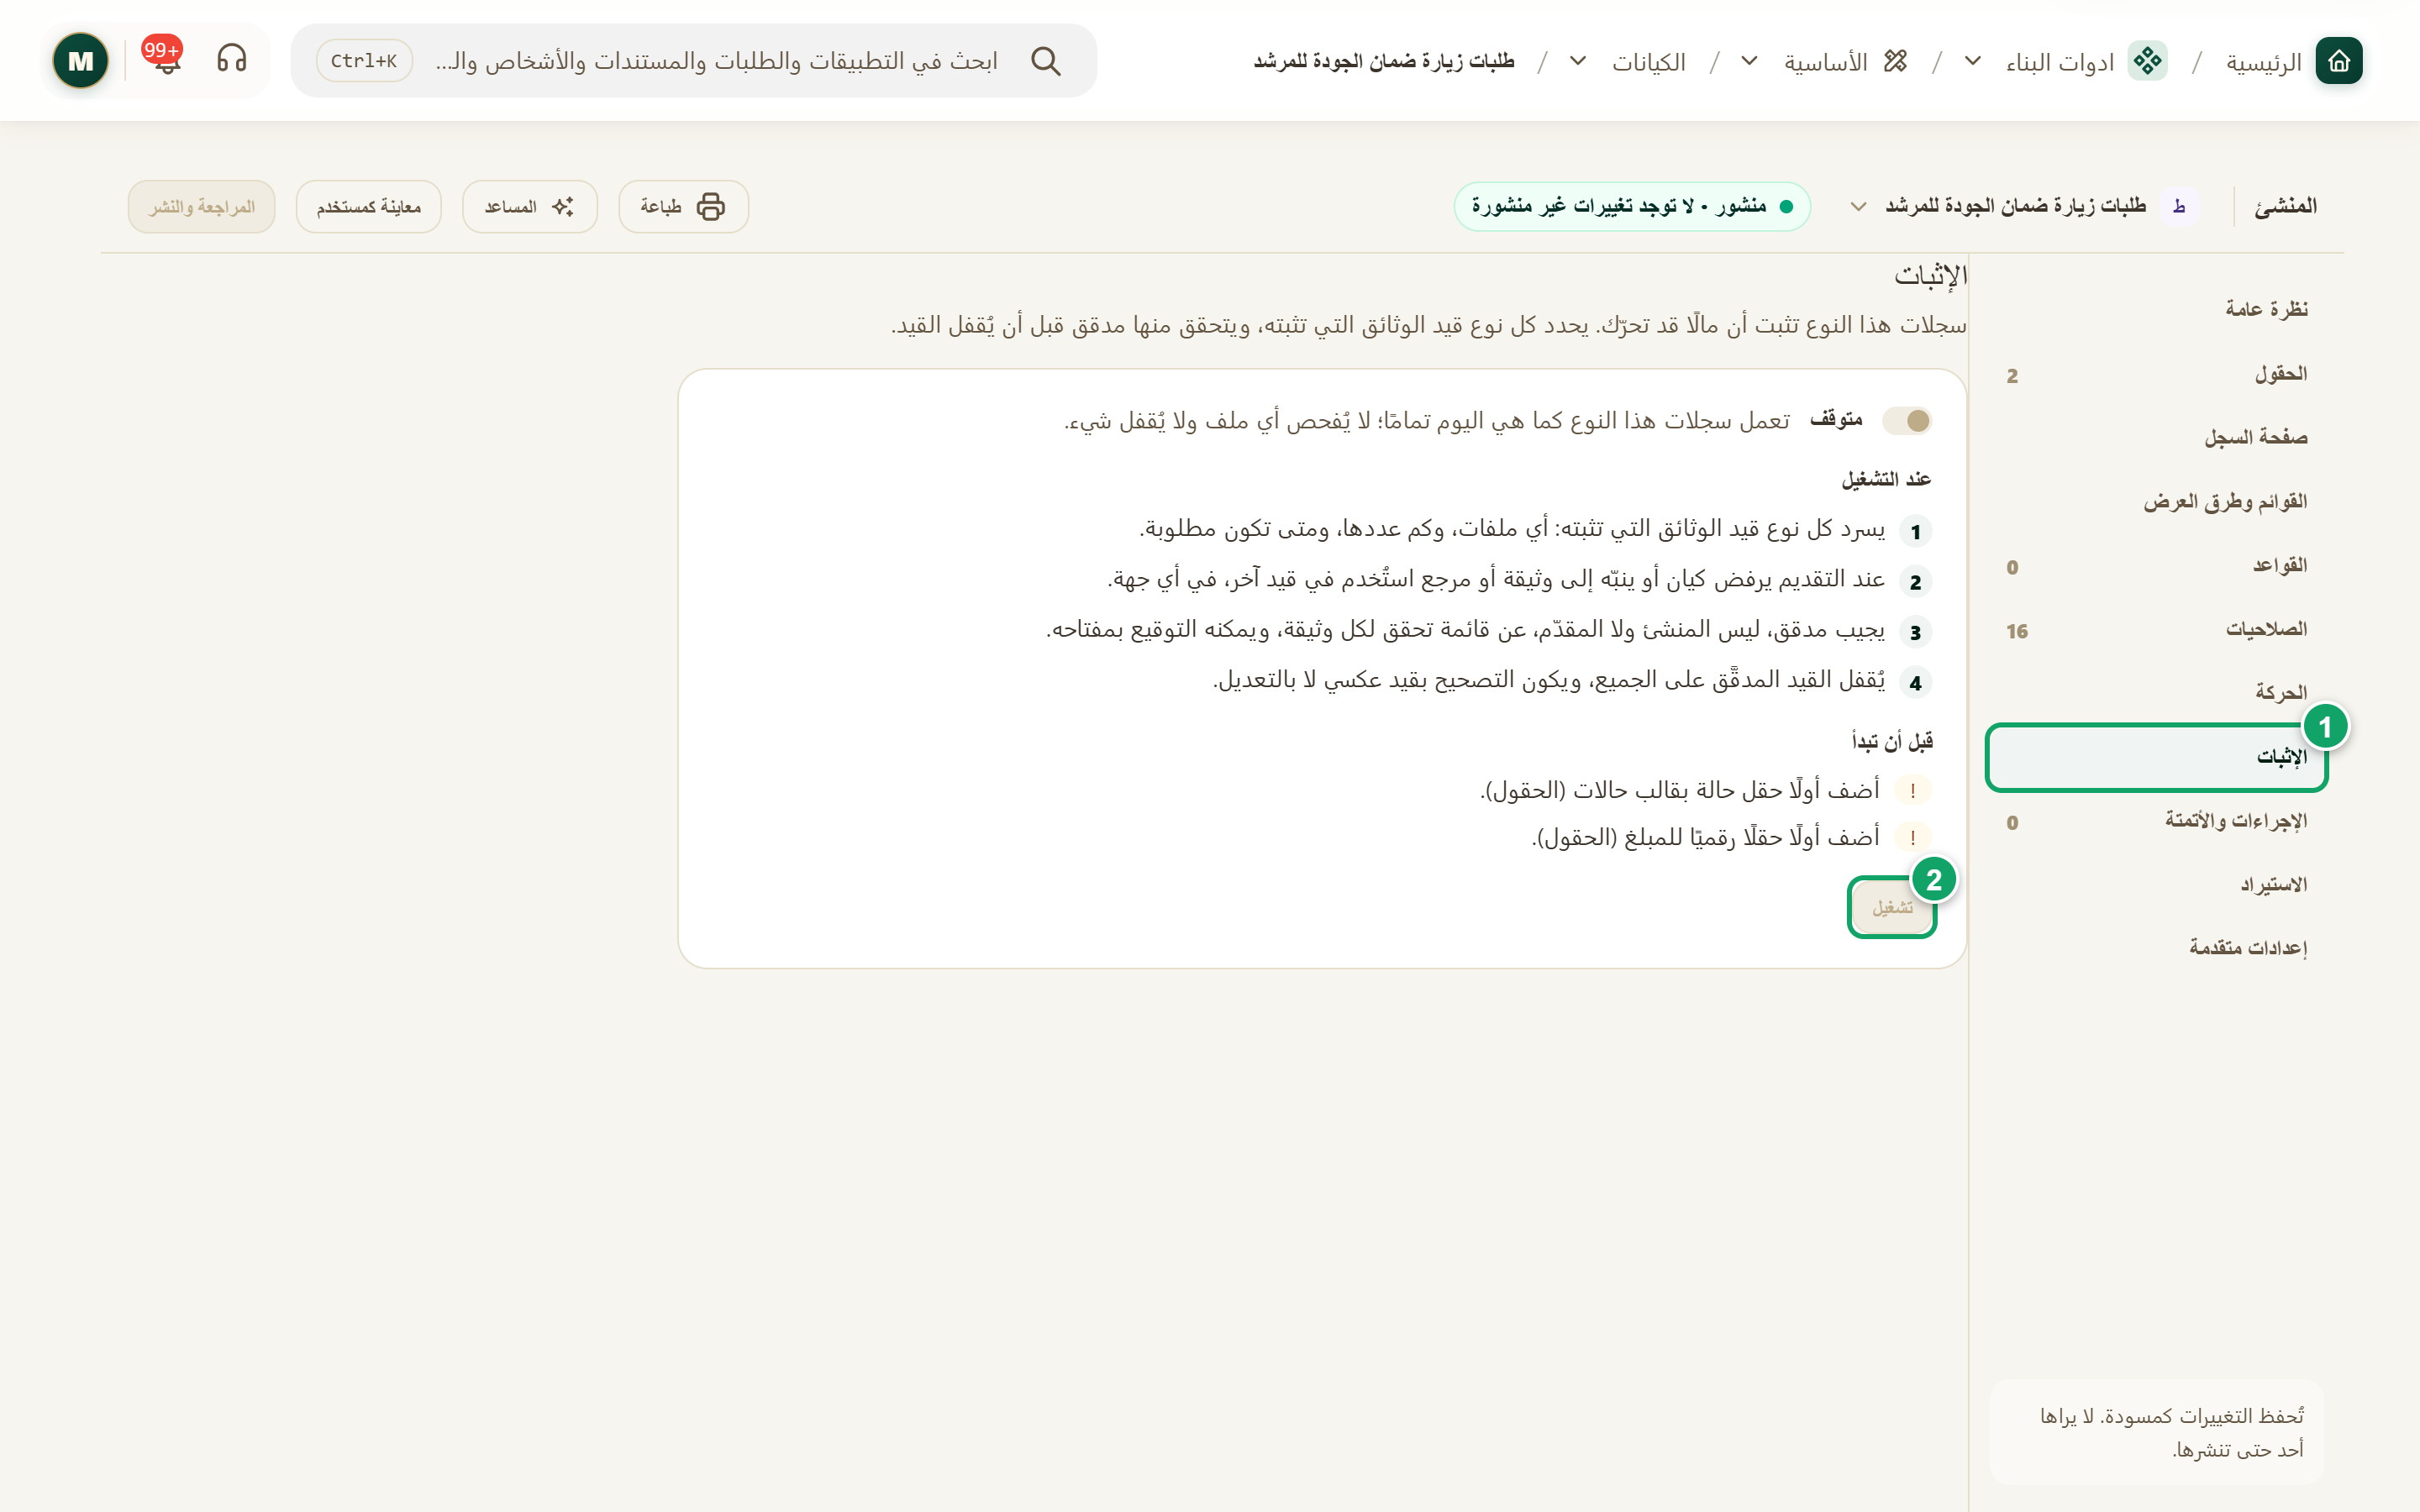
\includegraphics[width=0.95\linewidth,height=0.72\textheight,keepaspectratio]{figures/screens/ch06-ws-evidence-ar.png}
\caption{قسم «الإثبات» قبل تشغيله في نوع سجلات اختباري}
\label{fig:builder-evidence-screen}
\shotnote{تعرض الصورة القسم في النوع الاختباري على test2 وهو «متوقف»، مع شرح ما يحدث عند التشغيل وقائمة «قبل أن تبدأ». ويبيّن ذلك أن الزر يبقى معطلاً حتى يكتمل الشرطان، لأن هذا النوع لا يحوي حقل حالة ولا حقلاً رقمياً للمبلغ. ① «الإثبات» في القائمة الجانبية. ② «تشغيل»: يفعّل الإثبات بعد استيفاء الشروط.}
\end{figure}

\begin{table}[H]
\centering
\caption{تبويبات «الإثبات» بعد التشغيل}
\label{tab:builder-evidence-tabs}
\begin{tabularx}{\linewidth}{R{3.6cm} Y}
\rcHeaderRow
\thh{التبويب} & \thh{ما تضبطه فيه}\\
أنواع القيود والوثائق & في «عام»: «حقل الحالة» و«حالة التقديم» و«حالة التدقيق» و«حالات الإعادة»، و«حقل نوع القيد» عندما تختلف الوثائق حسب نوع القيد، و«حقول القيد» (المبلغ إلزامي، والعملة وتاريخ القيمة والجهة والطرف المقابل اختيارية)، و«الترقيم» ببادئة. ثم أنواع القيود، ولكل نوع «الفحوص المتقاطعة» و«وثائق الإثبات».\\
التكرار & قواعد تقارن كل قيد مقدَّم بقيود النوع حسب «محتوى الملف» أو «الحقول» أو «القراءة الآلية»، في «الجهة نفسها» أو «المؤسسة كلها»، ثم تختار «رفض» أو «تنبيه مع سبب» أو «إشارة للمدقق». وعند تطابق أكثر من قاعدة تغلب النتيجة الأشد.\\
القراءة الآلية & تقرأ الآلة من الوثائق قيماً مثل «المبلغ الإجمالي» و«رقم الوثيقة»، فتقترحها أو تقارنها بما أدخله المقدّم، ضمن «السقف الشهري» و«الصفحات لكل ملف».\\
الترحيل & يعرض «دورة الحياة» من التقديم إلى الإعادة أو التدقيق، ويفحص قالب الحالات وتوافقه مع قسم «الحركة». ودون إعداد للحركة تُثبت القيود وتُدقَّق ولا يتحرك أي مبلغ.\\
السرية & «المستوى الافتراضي» للوثائق، و«توقيع المدقق» بمفتاح العضو، و«قابلة للتعديل بعد التدقيق» للحقول التي تبقى مفتوحة بعد القفل، مثل الملاحظات. أما وثائق المستوى «سري (3)» فما فوق فتُعرض فقط، ولا تُنزَّل ولا تُرسل إلى القراءة الآلية.\\
\end{tabularx}
\end{table}

\begin{table}[H]
\centering
\caption{إعدادات كل وثيقة}
\label{tab:builder-evidence-slot}
\begin{tabularx}{\linewidth}{R{3.6cm} Y}
\rcHeaderRow
\thh{الإعداد} & \thh{المعنى}\\
مطلوبة & «دائمًا»، أو «اختيارية»، أو «عندما…» يتحقق شرط يُفحص عند التقديم ثم عند التدقيق.\\
الملفات & الصيغ المقبولة: \en{PDF} والصور و\en{Word} و\en{Excel}، وعدد الملفات «على الأقل» و«على الأكثر»، و«الحجم الأقصى (ميغابايت)»، وحد أدنى لدقة الصور. وإذا لم تختر صيغة، فتُقبل ملفات \en{PDF} والصور.\\
وثيقة مشتركة & «يمكن أن تثبت قيودًا أخرى» عندما تغطي وثيقة واحدة أكثر من قيد، مثل الأقساط.\\
السرية والقراءة & مستوى سرية خاص بالوثيقة، و«تُقرأ هذه الوثيقة آليًا».\\
قائمة تحقق المدقق & بنود يجيب عنها المدقق بنعم أو لا أو لا ينطبق مع ملاحظة، ولا يكتمل التدقيق إلا إذا كانت كل الإجابات نعم أو لا ينطبق.\\
\end{tabularx}
\end{table}

\begin{rcwarn}[الإيقاف لا يمحو ما قُدّم]
إذا أوقفت الإثبات بعد تقديم قيود، فيحتفظ كيان بإعداده ويعرض القسم «متوقف» مع زر «إعادة التشغيل»، ويبقى سجل القيود وأقفالها كما هي. ولا تُحذف ملفات الإثبات أبداً، فحتى القيد المعاد يحتفظ بملفاته القديمة بجانب الجديدة.
\end{rcwarn}

\subsection{قوائم التحقق بالأدلة}

يناسب «الإثبات» القيود المالية فقط. أما إذا أردت قائمة بنود يُجاب عنها داخل السجل، ويحتاج بعضها إلى صورة أو ملف دليلاً، مثل قائمة تحقق زيارة، فاجعلها سجلات مرتبطة واضبطها من حقل «علاقة» في نوع البنود: اختر «عرض العلاقة في التبويب»، ثم «قائمة تحقق» في «طريقة عرض العلاقات». وبعد ذلك تحدد «حقل الإجابة»، وتختار ضمن «ملفات الأدلة» قيمة «مجموعة الملفات» التي تُرفع إليها الأدلة، وتضيف شرطاً في «الأدلة مطلوبة فقط عندما…» إن لزم.

\begin{figure}[H]
\centering
\begin{tikzpicture}[node distance=0.5cm]
\node[stepBox] (a) {\RL{حقل حالة وحقل مبلغ}};
\node[stepBox,below=of a] (b) {\RL{تشغيل الإثبات}};
\node[stepBox,below=of b] (c) {\RL{أنواع القيود والوثائق}};
\node[stepBox,below=of c] (d) {\RL{التكرار والسرية}};
\node[stepBox,below=of d] (e) {\RL{الترحيل مع الحركة}};
\node[stepBox,below=of e] (f) {\RL{المراجعة والنشر}};
\draw[flowsTo] (a) -- (b);
\draw[flowsTo] (b) -- (c);
\draw[flowsTo] (c) -- (d);
\draw[flowsTo] (d) -- (e);
\draw[flowsTo] (e) -- (f);
\end{tikzpicture}
\rclegend
\caption{تشغيل الإثبات وضبطه}
\label{fig:builder-evidence-flow}
\shotnote{يبدأ المخطط بالحقلين لأن زر التشغيل يبقى معطلاً دونهما، ولأن كيان يستنتج منهما حالات التقديم والتدقيق وحقل المبلغ. ويأتي الترحيل قبل النشر لأن كيان يرفض النشر إذا لم يتوافق الإثبات مع إعداد «الحركة»، فالمال لا يتحرك إلا بعد التدقيق.}
\end{figure}

\subsection{خطوات العمل والتحقق}
\begin{enumerate}
\item تأكد في «الحقول» من وجود حقل «الحالة» بـ«قالب ثابت» منشور فيه حالة للتقديم وأخرى للتدقيق، ومن وجود حقل «رقم» للمبلغ.
\item افتح «الإثبات» واضغط «تشغيل»، ثم راجع في «عام» الحالات التي اقترحها كيان، واختر «حقول القيد» و«البادئة».
\item في «وثائق الإثبات» اضغط «إضافة وثيقة» لكل وثيقة، وحدد «مطلوبة» والملفات، ثم أضف بنود «قائمة تحقق المدقق» بزر «إضافة بند».
\item راجع «التكرار» و«السرية»، ثم افتح «الترحيل» وعالج كل فحص لم يتحقق، ولا سيما إذا كان للنوع إعداد في «الحركة».
\item انشر التغييرات، ثم أنشئ سجلاً تجريبياً، وارفع وثائقه من تبويب «الإثبات»، واضغط «تقديم للتدقيق»، واطلب من مستخدم آخر أن يدققه.
\end{enumerate}

\textbf{تحقق ومعالجة المشكلة:} يجب أن تظهر شارة «جاهز» بجانب عنوان القسم، وأن يحمل القيد المقدَّم رقماً يبدأ ببادئتك. فإذا بقي زر «تشغيل» معطلاً، فأضف الحقل الذي تشير إليه «قبل أن تبدأ». وإذا ظهرت شارة بعدد المشكلات «للإصلاح» أو مشكلة «إعداد الإثبات» في «قبل النشر»، فافتح التبويب المعلَّم بالخطأ وأكمل ما ينقصه.

\clearpage
\section{الاستيراد}
\label{sec:builder-feature-import}

يحدد قسم «الاستيراد» كيف يحمّل الناس سجلات هذا النوع ويحدّثونها من ملفات Excel وCSV. وأهم ما فيه «مفاتيح الاستيراد»: حقل أو مجموعة حقول، مثل رمز أو رقم، يطابق بها كيان كل صف في الملف مع سجل موجود، فيحدّثه بدلاً من أن ينشئ نسخة مكررة. وعندما يكون الخيار متوقفاً، يعمل الاستيراد كالمعتاد ويخمّن المطابقة بالمعرّف أو الرمز أو الاسم.

\textbf{المسار ومن يستخدمه:} نوع السجلات ← «الاستيراد». يستخدمه من يبني نوع السجلات، قبل أن يبدأ الفريق تحديث السجلات من ملفات.

\begin{rcnote}[مثال: شركة الأفق]
يضيف مسؤول النظام مفتاح استيراد مبنياً على رقم الطلب \en{HZN-VR-0001}، فيرفع عمر حداد ملف Excel بمواعيد الزيارات المعدّلة، ويحدّث كيان الطلبات الموجودة نفسها دون إنشاء طلبات جديدة. ويضيف المفتاح من ② ثم يفحصه من ③.
\end{rcnote}

\begin{figure}[H]
\centering
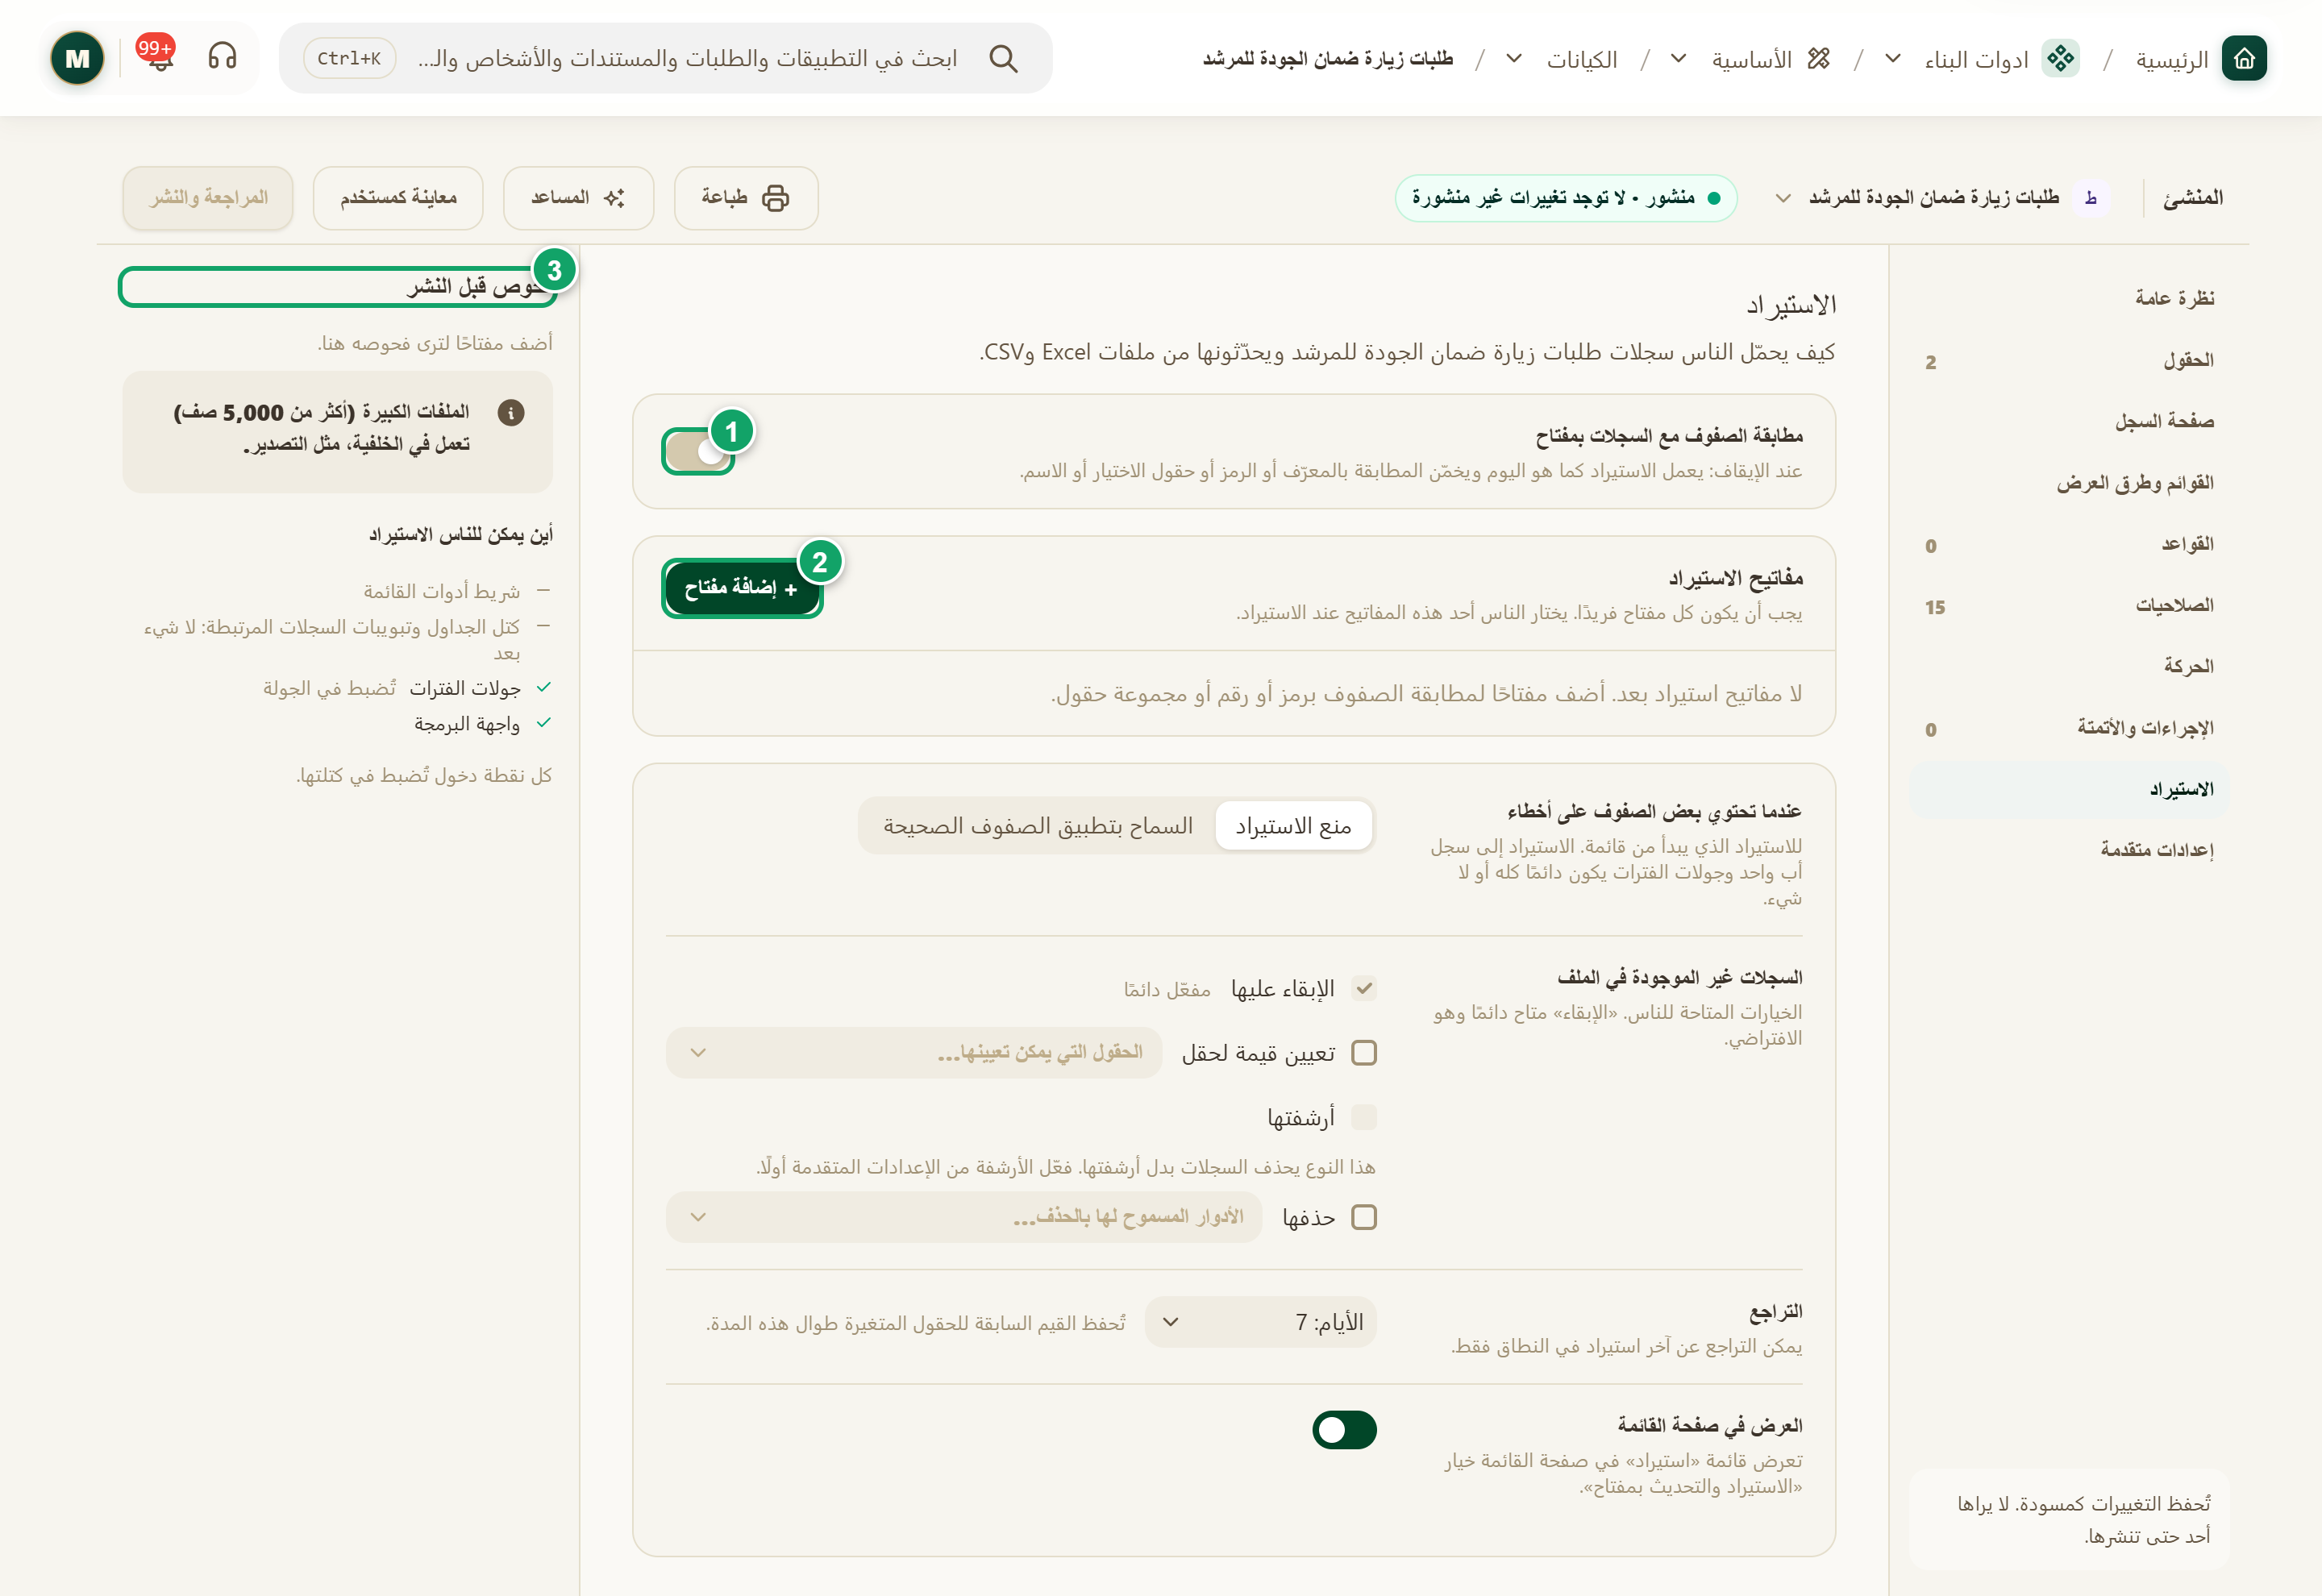
\includegraphics[width=0.95\linewidth,height=0.72\textheight,keepaspectratio]{figures/screens/ch06-ws-import-ar.png}
\caption{قسم «الاستيراد»}
\label{fig:builder-import-screen}
\shotnote{يحدد القسم طريقة تحديث السجلات من ملفات Excel وCSV، والمطابقة بالمفاتيح متوقفة هنا. ① مفتاح «مطابقة الصفوف مع السجلات بمفتاح». ② «+ إضافة مفتاح»: يضيف الحقل الذي تُطابق به الصفوف. ③ «فحوص قبل النشر»: تظهر فيها نتيجة «تشغيل الفحص» بعد إضافة مفتاح، لتتأكد من أنه فريد في السجلات المحفوظة.}
\end{figure}


\begin{table}[H]
\centering
\caption{ما الذي تجده هنا؟}
\label{tab:builder-import-data}
\begin{tabularx}{\linewidth}{R{3.6cm} Y}
\rcHeaderRow
\thh{الجزء} & \thh{المحتوى والإجراء}\\
مطابقة الصفوف مع السجلات بمفتاح & يفعّل الاستيراد بالمفاتيح. وعند الإيقاف يخمّن الاستيراد المطابقة كما في السابق.\\
مفاتيح الاستيراد & لكل مفتاح الحقول التي «يتكوّن من»ها، وأين يكون «فريد ضمن»ه، وطريقة «التوحيد» مثل تجاهل المسافات أو الأصفار البادئة، وهل هو «مدعوم بـ» قيمة فريدة، وحالته «جاهز» أو «مشكلة».\\
السلوك & ما يحدث «عندما تحتوي بعض الصفوف على أخطاء»: «منع الاستيراد» أو «السماح بتطبيق الصفوف الصحيحة»، وما يحدث لـ«السجلات غير الموجودة في الملف»: الإبقاء عليها أو أرشفتها أو حذفها، ومدة «التراجع» عن آخر استيراد.\\
فحوص قبل النشر & «تشغيل الفحص» يتأكد من أن المفتاح فريد في السجلات المحفوظة، ويعرض السجلات المتكررة أو الفارغة.\\
\end{tabularx}
\end{table}

\begin{figure}[H]
\centering
\begin{tikzpicture}[node distance=0.5cm]
\node[stepBox] (a) {\RL{إضافة مفتاح استيراد}};
\node[stepBox,below=of a] (b) {\RL{تشغيل الفحص}};
\node[stepBox,below=of b] (c) {\RL{ضبط السلوك}};
\node[stepBox,below=of c] (d) {\RL{النشر ثم استيراد ملف}};
\draw[flowsTo] (a) -- (b);
\draw[flowsTo] (b) -- (c);
\draw[flowsTo] (c) -- (d);
\end{tikzpicture}
\rclegend
\caption{تجهيز الاستيراد بالمفاتيح}
\label{fig:builder-import-flow}
\shotnote{يضع المخطط الفحص بعد إضافة المفتاح مباشرة، لأن المفتاح الذي تتكرر قيمته بين سجلين لا يعرف أيهما يحدّث. ثم تحدد ما يحدث للأخطاء والسجلات الغائبة عن الملف، لأن الاختيار الخاطئ هنا قد يؤرشف سجلات أو يحذفها. ولا يعمل شيء من ذلك قبل النشر.}
\end{figure}

\subsection{خطوات العمل والتحقق}
\begin{enumerate}
\item افتح نوع السجلات واختر «الاستيراد»، ثم فعّل «مطابقة الصفوف مع السجلات بمفتاح».
\item اضغط «+ إضافة مفتاح»، واختر الحقل الذي يميّز كل سجل، مثل الرمز أو الرقم التسلسلي.
\item اضغط «تشغيل الفحص»، وعالج أي سجلات متكررة أو فارغة يظهرها.
\item اختر السلوك المناسب للأخطاء والسجلات الغائبة، ثم انشر التغييرات.
\end{enumerate}

\textbf{تحقق ومعالجة المشكلة:} يجب أن تظهر حالة المفتاح «جاهز» وأن يظهر في الفحص أنه فريد. فإذا ظهر أن بعض السجلات ستتشارك المفتاح نفسه، فصحّح قيمها أولاً. ولا تختر حذف السجلات الغائبة عن الملف إلا عن قصد، واستخدم «التراجع» إذا أخطأ استيراد.

\clearpage
\section{إعدادات متقدمة}
\label{sec:builder-feature-advanced}

تضم «إعدادات متقدمة» إعدادات نادراً ما تتغير بعد البداية، مثل اسم السجل في القوائم، ومنع التكرار، والتسلسل بين السجلات، والتطبيق الذي يظهر فيه النوع. وهي جزء من المسودة مثل بقية الأقسام، فلا تصل إلى الفريق قبل النشر.

\textbf{المسار ومن يستخدمه:} نوع السجلات ← «إعدادات متقدمة». يستخدمه من يبني النوع، غالباً عند إنشائه ثم عند الحاجة فقط.

\begin{rcnote}[مثال: شركة الأفق]
يجعل مسؤول النظام «اسم السجل» في طلبات الزيارة هو الرقم التسلسلي مع اسم الفرع، ويضع النوع في تطبيق «خدمات الفروع»، ويختار «أرشفة السجلات بدل حذفها» حتى لا يضيع أي طلب. وتطابق اختياراته الرقمين ① و④.
\end{rcnote}

\begin{figure}[H]
\centering
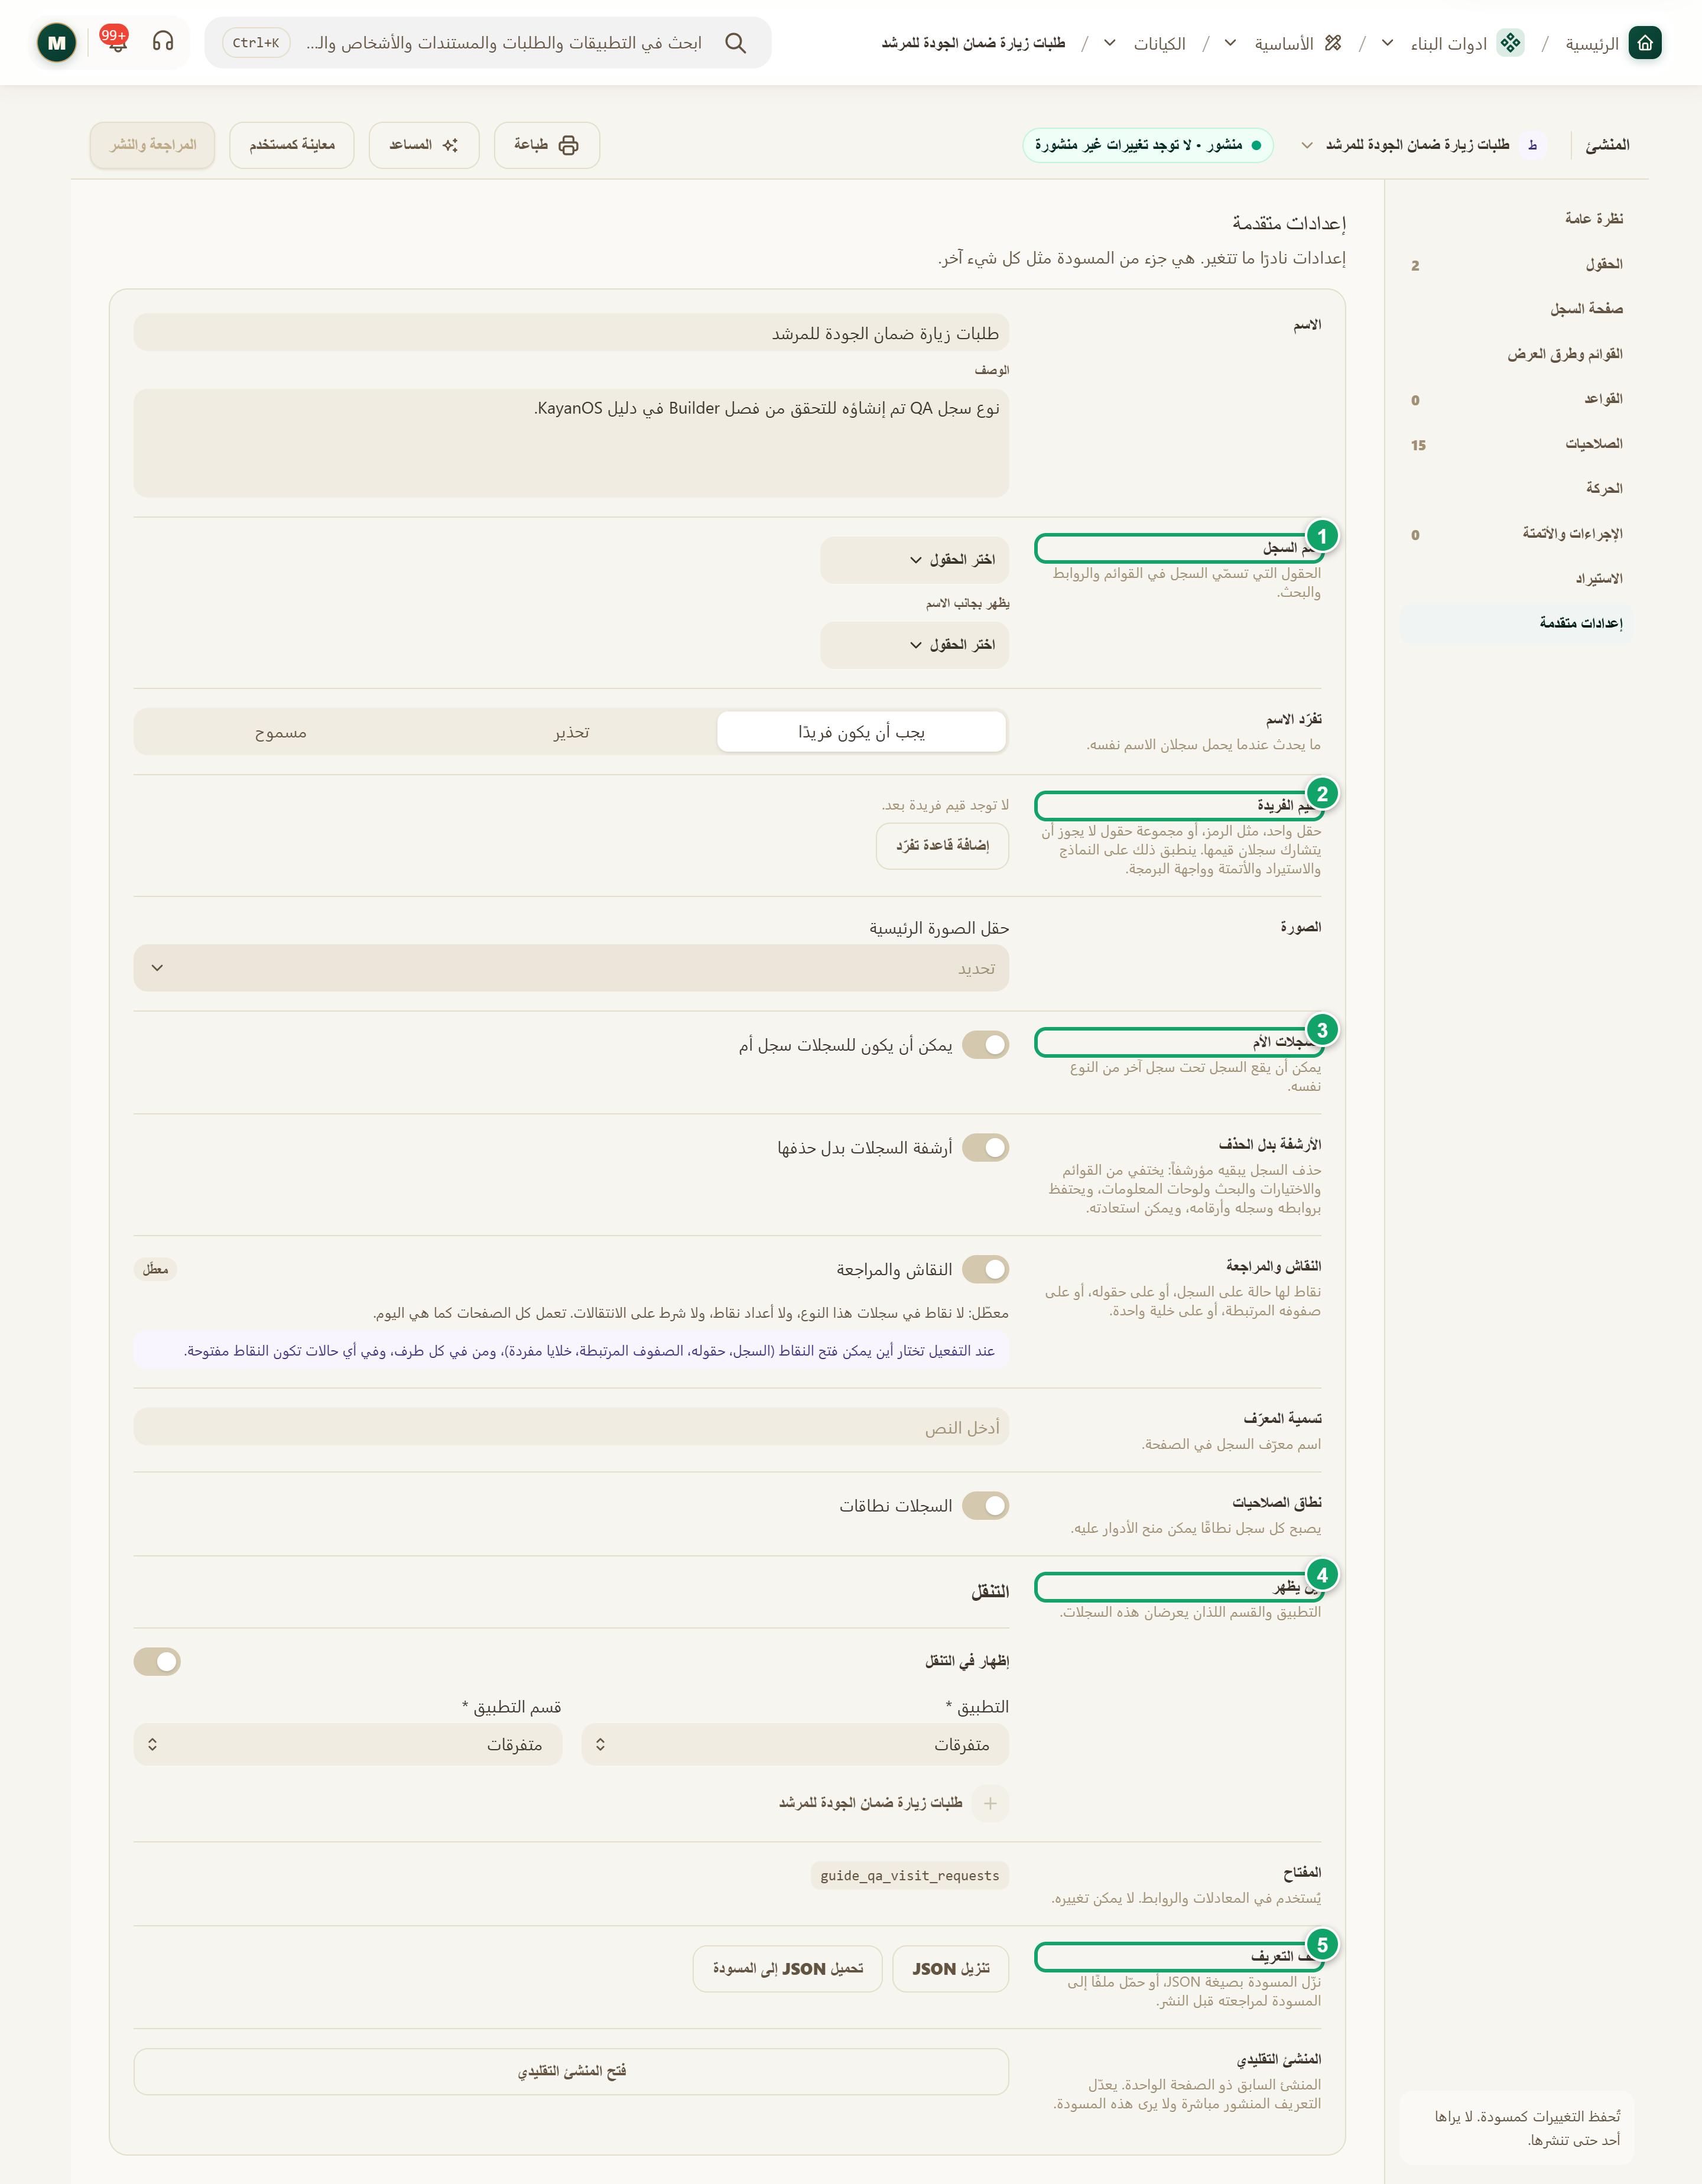
\includegraphics[width=0.95\linewidth,height=0.72\textheight,keepaspectratio]{figures/screens/ch06-ws-advanced-ar.png}
\caption{قسم «إعدادات متقدمة»}
\label{fig:builder-advanced-screen}
\shotnote{يجمع القسم إعدادات نادراً ما تتغير، ويظهر هنا لنوع السجلات الاختباري. ① «اسم السجل»: الحقول التي تسمّي السجل. ② «القيم الفريدة»: تمنع تكرار رمز أو مجموعة قيم. ③ «السجلات الأم»: تسمح بتسلسل أب وأبناء. ④ «أين يظهر»: التطبيق والقسم. ⑤ «ملف التعريف»: تنزيل الإعداد أو تحميله بصيغة JSON.}
\end{figure}


\begin{table}[H]
\centering
\caption{ما الذي تجده هنا؟}
\label{tab:builder-advanced-data}
\begin{tabularx}{\linewidth}{R{3.6cm} Y}
\rcHeaderRow
\thh{الإعداد} & \thh{المعنى}\\
اسم السجل & الحقول التي تسمّي السجل في القوائم والروابط والبحث، وحقل اختياري «يظهر بجانب الاسم».\\
تفرّد الاسم & ما يحدث عندما يحمل سجلان الاسم نفسه: «يجب أن يكون فريدًا» أو «تحذير» أو «مسموح».\\
القيم الفريدة & حقل، مثل الرمز، أو مجموعة حقول لا يجوز أن يتشارك سجلان قيمها، في النماذج والاستيراد والأتمتة أيضاً.\\
الصورة & الحقل الذي يُستخدم صورةً رئيسية للسجل.\\
السجلات الأم & تسمح بأن يقع السجل تحت سجل آخر من النوع نفسه، فتظهر طريقة العرض «شجرة».\\
الأرشفة بدل الحذف & يبقى السجل المحذوف مؤرشفاً: يختفي من القوائم والبحث، ويحتفظ بروابطه وأرقامه، ويمكن استعادته. ويمكنك أن تؤرشف معه سجلاته الفرعية والمهام المرتبطة به.\\
النقاش والمراجعة & يسمح بفتح نقاط لها حالة على السجل أو حقوله أو صفوفه المرتبطة أو خلية واحدة، فتظهر في تبويب «النقاط» في صفحة السجل. ويبقى متوقفاً حتى تشغّله.\\
تسمية المعرّف & اسم معرّف السجل في الصفحة.\\
نطاق الصلاحيات & يجعل كل سجل نطاقاً يمكن منح الأدوار عليه، مثل منح مدير فرع صلاحية على فرعه فقط.\\
أين يظهر & «التطبيق» و«قسم التطبيق» اللذان يعرضان السجلات، و«إظهار في التنقل»، والأيقونة.\\
المفتاح & يُستخدم في المعادلات والروابط، ولا يمكن تغييره.\\
ملف التعريف & «تنزيل JSON» لنسخة من المسودة، أو «تحميل JSON إلى المسودة» لمراجعته قبل النشر.\\
المنشئ التقليدي & المنشئ السابق ذو الصفحة الواحدة؛ يعدّل التعريف المنشور مباشرة ولا يرى المسودة، فاستخدمه بحذر.\\
\end{tabularx}
\end{table}

\begin{figure}[H]
\centering
\begin{tikzpicture}[node distance=0.5cm]
\node[entity] (adv) {\RL{إعدادات متقدمة}};
\node[entityOpt,below right=0.7cm and 0.3cm of adv] (tree) {\RL{السجلات الأم}};
\node[entityOpt,below left=0.7cm and 0.3cm of adv] (scope) {\RL{نطاق الصلاحيات}};
\node[entityOpt,below=0.7cm of tree] (treeview) {\RL{عرض الشجرة}};
\node[entityOpt,below=0.7cm of scope] (roles) {\RL{أدوار على سجل واحد}};
\draw[dependsOnOpt] (adv.south) -- ++(0,-0.3) -| (tree.north);
\draw[dependsOnOpt] (adv.south) -- ++(0,-0.3) -| (scope.north);
\draw[dependsOnOpt] (tree) -- (treeview);
\draw[dependsOnOpt] (scope) -- (roles);
\end{tikzpicture}
\rclegend
\caption{إعدادان يفتحان إمكانات أخرى}
\label{fig:builder-advanced-effects}
\shotnote{يوضّح الشكل أن بعض الإعدادات المتقدمة شرط لإمكانات في أقسام أخرى: فتفعيل «السجلات الأم» يتيح عرض «شجرة» في القوائم، وتفعيل «نطاق الصلاحيات» يتيح منح أدوار على سجل واحد. لذلك إذا لم تجد إحدى هذه الإمكانات، فابدأ بمراجعة هذا القسم.}
\end{figure}

\subsection{خطوات العمل والتحقق}
\begin{enumerate}
\item افتح نوع السجلات واختر «إعدادات متقدمة».
\item اختر «اسم السجل» من حقول تميّز السجل فعلاً، مثل الرقم التسلسلي.
\item أضف «قاعدة تفرّد» للحقول التي يجب ألا تتكرر، وراجع التحذير إن وُجدت تكرارات حالية.
\item راجع «أين يظهر» لتتأكد من التطبيق والقسم، ثم انشر التغييرات.
\end{enumerate}

\textbf{تحقق ومعالجة المشكلة:} بعد النشر يجب أن تظهر السجلات في القوائم والبحث بالاسم الذي اخترته، وأن يُرفض إدخال قيمة فريدة مكررة. وقبل أي تعديل كبير، استخدم «تنزيل JSON» لتحتفظ بنسخة من الإعداد.

\clearpage
\section{المراجعة والنشر}
\label{sec:builder-feature-publish}

يحفظ «المنشئ» كل تعديل تجريه مسودةً، ولا يرى أحد غيرك هذه التغييرات حتى تنشرها. وتعرض «المراجعة والنشر» التغييرات كلها قبل النشر، وتمنعه إذا بقيت مشكلة يجب حلها. وكل نشر يُنشئ إصداراً جديداً يمكنك الرجوع إليه لاحقاً.

\textbf{المسار ومن يستخدمه:} نوع السجلات ← «المراجعة والنشر». يستخدمه من يبني النوع بعد أن ينهي مجموعة من التعديلات.

\begin{rcnote}[مثال: شركة الأفق]
قبل إطلاق «طلبات الزيارة» يستخدم مسؤول النظام «معاينة كمستخدم» ليرى الصفحة كما يراها عمر حداد، ثم ينشر الإصدار الأول، ويطلب من عمر تجربة طلب لزيارة فرع حلب. ويستخدم ③ قبل أن ينشر من ④.
\end{rcnote}

\begin{figure}[H]
\centering
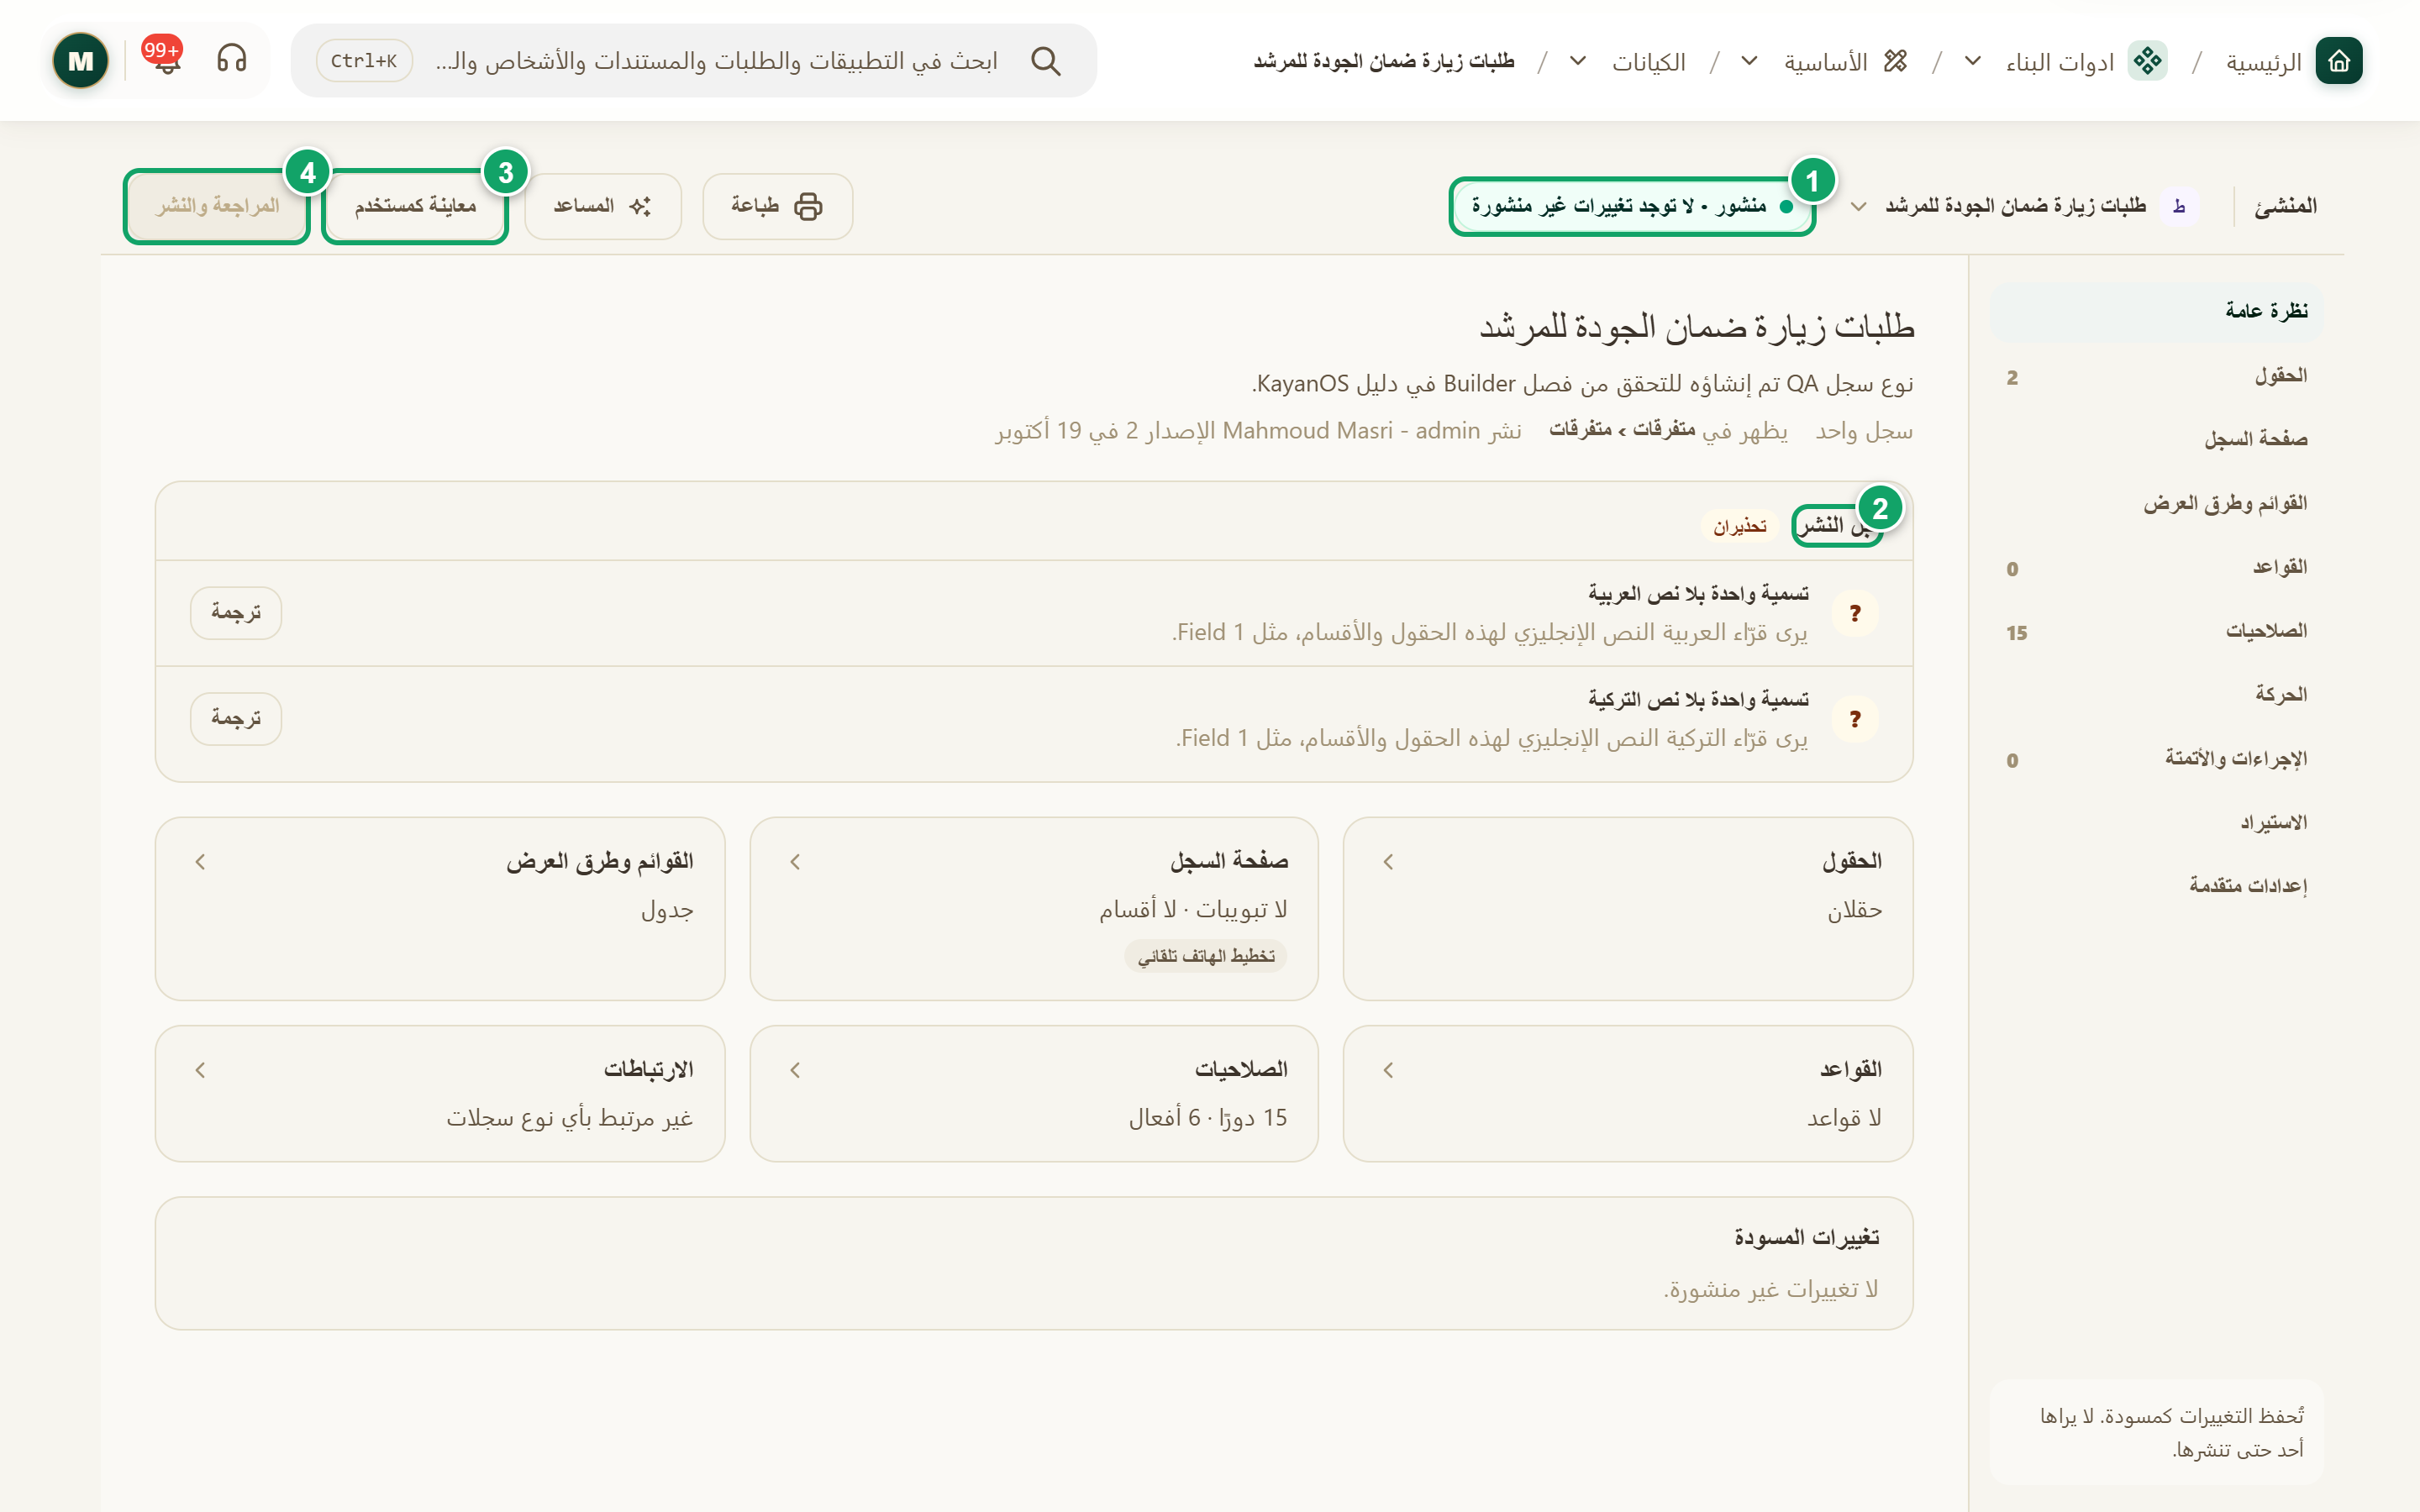
\includegraphics[width=0.95\linewidth,height=0.72\textheight,keepaspectratio]{figures/screens/ch06-ws-overview-ar.png}
\caption{«نظرة عامة» بعد النشر}
\label{fig:builder-publish-screen}
\shotnote{تلخّص «نظرة عامة» حالة النوع وما يجب إصلاحه قبل النشر. والنوع الاختباري هنا منشور في الإصدار 2 بعد اختبار هذا الفصل، وتبقى تحذيرات ترجمة لا تمنع النشر. ① الحالة: «منشور · لا توجد تغييرات غير منشورة». ② «قبل النشر»: المشكلات والتحذيرات. ③ «معاينة كمستخدم». ④ «المراجعة والنشر»: يفتح قائمة التغييرات وزر النشر.}
\end{figure}


\begin{table}[H]
\centering
\caption{ما الذي تجده هنا؟}
\label{tab:builder-publish-data}
\begin{tabularx}{\linewidth}{R{3.6cm} Y}
\rcHeaderRow
\thh{العنصر} & \thh{المعنى والإجراء}\\
مسودة & حالة النوع وفيه تغييرات لم تُنشر. أما «منشور · لا توجد تغييرات غير منشورة» فيعني أن ما يراه الفريق هو آخر ما بنيته.\\
نظرة عامة & ملخص الحقول والصفحة والقوائم والقواعد، و«قبل النشر» تعرض المشكلات التي تمنع النشر والتحذيرات.\\
معاينة كمستخدم & تعرض النوع كما سيراه المستخدم قبل النشر.\\
المراجعة والنشر & تفتح نافذة «مراجعة التغييرات» التي تجمع التغييرات حسب القسم، ولكل تغيير خانة اختيار تستطيع إلغاءها فيبقى في المسودة. وتكتب وصفاً اختيارياً للإصدار، ثم تضغط «نشر N تغيير».\\
تغييرات معلّقة & إذا فعّلت المؤسسة اعتماد تغييرات أنواع السجلات، فلا تُطبَّق التغييرات التي تشملها سياسة الاعتماد عند النشر، بل تُحفظ «تغييرات معلّقة» ترسلها للاعتماد من الشريط أعلى المنشئ. ويبقى النوع وسجلاته يعملان بالتعريف الحالي حتى تُعتمد وتُطبَّق.\\
سجل الإصدارات & يعرض الإصدارات السابقة. و«استعادة» إصدار تضع حقوله وتخطيط صفحته في المسودة، ولا يصل شيء إلى الفريق حتى تنشر.\\
تجاهل المسودة & يزيل التغييرات غير المنشورة للجميع، ويبقى التعريف المنشور كما هو.\\
\end{tabularx}
\end{table}

\begin{figure}[H]
\centering
\begin{tikzpicture}[node distance=0.5cm]
\node[stepBox] (a) {\RL{تعديلات تُحفظ مسودة}};
\node[stepBox,below=of a] (b) {\RL{حل مشكلات «قبل النشر»}};
\node[stepBox,below=of b] (c) {\RL{معاينة كمستخدم}};
\node[stepBox,below=of c] (d) {\RL{النشر: إصدار جديد}};
\draw[flowsTo] (a) -- (b);
\draw[flowsTo] (b) -- (c);
\draw[flowsTo] (c) -- (d);
\end{tikzpicture}
\rclegend
\caption{من المسودة إلى الإصدار المنشور}
\label{fig:builder-publish-flow}
\shotnote{يبيّن المخطط أن النشر خطوة مقصودة يتخذها من يبني النوع، لا نتيجة تلقائية للحفظ. فالمسودة تجمع التعديلات بأمان، ولا يصل أي منها إلى الفريق قبل حل المشكلات والنشر، ويصبح كل نشر إصداراً يمكن استعادته.}
\end{figure}

\subsection{خطوات العمل والتحقق}
\begin{enumerate}
\item افتح «نظرة عامة» وراجع «قبل النشر»، ثم أصلح كل مشكلة تمنع النشر.
\item اضغط «معاينة كمستخدم» وراجع الصفحة والقوائم كما سيراها الفريق.
\item اضغط «المراجعة والنشر»، وراجع قائمة التغييرات، وألغِ اختيار أي تغيير تريد إبقاءه في المسودة، ثم اضغط «نشر N تغيير».
\item أنشئ سجلاً تجريبياً من قائمة النوع، ثم أعد فتحه وتأكد من حفظ قيمه.
\end{enumerate}

\textbf{تحقق ومعالجة المشكلة:} يجب أن تظهر رسالة بأن النوع «نُشر كإصدار» برقمه، وأن تتغير الحالة إلى «منشور · لا توجد تغييرات غير منشورة». فإذا ظهرت مشكلة بعد النشر، فافتح «سجل الإصدارات» واستعد الإصدار السابق إلى المسودة، ثم صحّحها وانشرها من جديد، لأن الاستعادة وحدها لا تغيّر ما يراه الفريق.
